% !TeX spellcheck = en_GB
%% 
%% Copyright 2019-2024 Elsevier Ltd
%% 
%% Version 2.4
%% 
%% This file is part of the 'CAS Bundle'.
%% --------------------------------------
%% 
%% It may be distributed under the conditions of the LaTeX Project Public
%% License, either version 1.2 of this license or (at your option) any
%% later version.  The latest version of this license is in
%%    http://www.latex-project.org/lppl.txt
%% and version 1.2 or later is part of all distributions of LaTeX
%% version 1999/12/01 or later.
%% 
%% The list of all files belonging to the 'CAS Bundle' is
%% given in the file `manifest.txt'.
%% 
%% Template article for cas-dc documentclass for 
%% double column output.

%\documentclass[a4paper,fleqn,longmktitle]{cas-dc}
\documentclass[a4paper,fleqn]{cas-dc}

%\usepackage[authoryear,longnamesfirst]{natbib}
%\usepackage[authoryear]{natbib}
\usepackage[numbers]{natbib}

%%%Author definitions
\def\tsc#1{\csdef{#1}{\textsc{\lowercase{#1}}\xspace}}
\tsc{WGM}
\tsc{QE}
\tsc{EP}
\tsc{PMS}
\tsc{BEC}
\tsc{DE}

\newcommand{\accuracy}{A}
\newcommand{\precision}{P}
\newcommand{\recall}{R}
\newcommand{\FOne}{F_1}
\newcommand{\MacroFOne}{\overline{\FOne}}

\newcommand{\positiveclass}{p}
\newcommand{\negativeclass}{n} 

\newcommand{\ksTP}{[\positiveclass \to \positiveclass]}
\newcommand{\ksFP}{[\negativeclass \to \positiveclass]}
\newcommand{\ksTN}{[\negativeclass \to \negativeclass]}
\newcommand{\ksFN}{[\positiveclass \to \negativeclass]}
\newcommand{\ksOriginalPositive}{[\positiveclass\to]}
\newcommand{\ksOriginalNegative}{[\negativeclass\to]} 
\newcommand{\ksPredictedPositive}{[\to\positiveclass]}
\newcommand{\ksPredictedNegative}{[\to\negativeclass]}
\newcommand{\ksAll}{[\to]} 




\newcommand{\TP}{\mathrm{TP}}
\newcommand{\FP}{\mathrm{FP}}
\newcommand{\TN}{\mathrm{TN}}
\newcommand{\FN}{\mathrm{FN}}



% Put your packages, macros, setting here.

%%%% REMARK LIST GENERATOR %%%%%%%%%

%\usepackage{tikz}
%\usepackage{manfnt}   % dangerous sign 
\usepackage{color}
\definecolor{brickred}      {cmyk}{0   , 0.89, 0.94, 0.28}

\makeatletter \newcommand \kslistofremarks{\section*{Uwagi} \@starttoc{rks}}
  \newcommand\l@uwagas[2]
    {\par\noindent \textbf{#2:} %\parbox{10cm}
{#1}\par} \makeatother


\newcommand{\xyzremark}[3]{%
{%\marginpar{\textdbend}
{\color{#3}{[#2]}}}%
\addcontentsline{rks}{uwagas}{\protect{#1 #2}}%
}

\newcommand{\ksremark}[1]{\xyzremark{KS: }{#1}{brickred}}
\newcommand{\jsremark}[1]{\xyzremark{JS: }{#1}{green}}
%\newcommand{\nnremark}[1]{\xyzremark{NN: }{#1}{blue}}


%%%%%%%%%%%%%% END OF REMARK LIST GENERATOR %%%%%%%%%%%


\usepackage{subcaption}   % subfigures
\usepackage{tikz}
\usepackage{pgfplots}
\usepackage{siunitx}
\pgfplotsset{compat=1.18}

\usetikzlibrary{
	positioning,
	arrows.meta,
	shadows,
	backgrounds,
	fit,
	babel    
}

\definecolor{stepcolor}{HTML}{4A90E2} 
\definecolor{datacolor}{HTML}{50E3C2}
\definecolor{arrowcolor}{HTML}{333333}

\tikzset{
	stepnode/.style={
		draw=stepcolor!70!black,
		fill=stepcolor!15,
		rounded corners=4pt,
		minimum width=2.5cm,
		minimum height=0.9cm,
		drop shadow,
		thick,
		align=center,
		font=\sffamily\small
	},
	datanode/.style={
		draw=datacolor!70!black,
		fill=datacolor!15,
		shape=rectangle,
		minimum width=2.0cm,
		minimum height=0.8cm,
		thick,
		align=center,
		font=\sffamily\small
	},
	finalnode/.style={
		stepnode,
		fill=blue!10,
		draw=blue!50,
		font=\sffamily\small\bfseries
	},
	arrow/.style={
		->,
		>=Stealth,
		color=arrowcolor!80,
		line width=0.8pt,
	},
	dasharrow/.style={
		->,
		>=Stealth,
		dashed,
		color=arrowcolor!60,
		line width=0.7pt,
	}
}



\newcommand{\zscore}{Z}
\newcommand{\logreg}{LR}
\newcommand{\postag}[1]{\texttt{#1}}
\newcommand{\code}[1]{\texttt{#1}}

\newcommand{\customtfidf}{CTf-IDF}
\newcommand{\custombow}{CBoW}

\newcommand{\positive}{\rho}
\newcommand{\negative}{\eta}
\newcommand{\smoothedprob}[1]{s(#1)}
\newcommand{\Count}[1]{\|{#1}\|}

\newcommand{\vocabsize}{V}
\newcommand{\tokenclass}{\kappa}
\newcommand{\instanceClass}{c}
\newcommand{\insclass}{^{(\instanceClass)}}
\newcommand{\numbertokens}[1]{T_{#1}}
\newcommand{\smoothparam}{\beta}
\newcommand{\kconcepts}{k}
\newcommand{\conceptWeight}{w}
\newcommand{\inputtext}{X}

\newcommand{\mcnemarp}{p}
\newcommand{\mcnemarchi}{\chi^2}

\newcommand{\weightparam}{w}

\newcommand{\literal}[1]{\textit{`#1'}}

\newcommand{\predVal}{y}
\newcommand{\idx}{\iota}
\newcommand{\mBase}{B}
\newcommand{\mSpec}{S}
\newcommand{\mCas}{C}
\newcommand{\thresh}{\tau}
\newcommand{\numVal}{N}

\newcommand{\modelvar}{\mu}
\newcommand{\sweepthresh}{t}
\newcommand{\missclassified}[1]{n_{#1}}
\newcommand{\nullhypo}{H_0}

\newcommand{\probSmall}[1]{p_{#1}}
\newcommand{\probLarge}[2]{P_{#1}(\predVal=1 \mid #2)}

\newcommand{\accMask}[3]{A_{#1,#2}(#3)}
\newcommand{\coverage}[2]{\epsilon_{#1}(#2)}
\newcommand{\hybridacc}[2]{\aleph(#1,#2)}

\newcommand{\cascadePred}[3]{\hat{\predVal}_{#1,#2}^{\,\mCas}(#3)}
\newcommand{\baseProb}[2]{\probSmall{\mBase_{\!#1}}^{(#2)}}
\newcommand{\optimal}{o}


%%%

\begin{document}
\kslistofremarks
\clearpage

\tableofcontents
\clearpage	
	
	
\let\WriteBookmarks\relax
\def\floatpagepagefraction{1}
\def\textpagefraction{.001}
\shorttitle{Deciding with Conviction: A Granular Three-Way Cascade Framework for Efficient Sentiment Analysis}
\shortauthors{J. Supierz and K. Siminski}

\title [mode = title]{Deciding with Conviction: A Granular Three-Way Cascade Framework for Efficient Sentiment Analysis}                      
%\tnotemark[1,2]

%\tnotetext[1]{This document is the results of the research project funded by the National Science Foundation.}

%\tnotetext[2]{The second title footnote which is a longer text matter to fill through the whole text width and overflow into another line in the footnotes area of the first page.}

\author[1]{Jan Supierz}
\cormark[1]
%\fnmark[1]
\ead{js319212@student.polsl.pl}
\ead[url]{https://github.com/JanSupierz}
\credit{Conceptualization, Methodology, Software, Writing -- Original draft preparation}

\author[1]{Krzysztof Siminski}[orcid=0000-0002-6118-606X]
\cormark[2]
\ead{Krzysztof.Siminski@polsl.pl}
\ead[url]{https://github.com/ksiminski}
\credit{Supervision, Validation, Writing -- Review \& Editing}

%\address[1]{, Street 129, 1043 NX Amsterdam, The Netherlands}
\affiliation[1]{organization={Faculty of Automatic Control, Electronics and Computer Science, Silesian University of Technology},
                addressline={Akademicka 16}, 
                city={Gliwice},
              	 citysep={}, % Uncomment if no comma needed between city  and postcode
                postcode={44-100}, 
                country={Poland}}

\cortext[cor1]{Principal corresponding author}
\cortext[cor2]{Corresponding author}
%\fntext[fn1]{This is the first author footnote, but is common to third author as well.}
%\fntext[fn2]{Another author footnote, this is a very long footnote and it should be a really long footnote. But this footnote is not yet sufficiently long enough to make two lines of footnote text.}

%\nonumnote{This note has no numbers. In this work we demonstrate $a_b$ the formation Y\_1 of a new type of polariton on the interface between a cuprous oxide slab and a polystyrene micro-sphere placed on the slab. }

\begin{abstract}
Sentiment analysis models face a persistent trade‑off between the high accuracy of deep learning and the computational efficiency required for practical use.
This thesis investigates whether granular computing techniques can bridge this gap.
A statistical $\zscore$-score pruning method is proposed that discards non‑discriminative $n$-grams, shrinking the feature space by over $60\%$ while maintaining or improving classification accuracy (RQ1). Semantic concept clustering is explored as an alternative granulation strategy. Building on the best lightweight model, a cascade ensemble architecture is proposed: a linear support vector machine handles the majority of reviews with high confidence, and a specialist transformer model resolves only the uncertain cases (RQ2). All methods are evaluated on the IMDb movie review dataset. The cascade achieves a macro $\FOne$-score of approximately $92.3\%$, significantly outperforming both standalone baselines while delegating only $15\%$-$20\%$ of the test instances to the deep-learning specialist. These results demonstrate that granular vocabulary reduction and model‑level deferral can successfully balance accuracy and efficiency in sentiment analysis systems.
\end{abstract}

\begin{graphicalabstract}

\includegraphics{figs/cas-grabs.pdf}
\end{graphicalabstract}

\begin{highlights}
\item Research highlights item 1
\item Research highlights item 2
\item Research highlights item 3
\end{highlights}

\begin{keywords}
sentiment analysis \sep granular computing \sep cascade ensemble \sep machine learning \sep natural language processing
\end{keywords}


\maketitle

\ksremark{Proszę sobie założyć ORCID.}
\section{Introduction}
\label{sec:introduction}

The rapid growth of user-generated content on social media platforms, review portals, discussion forums, and e-commerce websites has created an unprecedented demand for automatic methods capable of extracting opinions from textual data. Sentiment analysis (SA) \jsremark{Czy akronimy powinny mieć wielkie litery? Sentiment \textbf{A}nalysys --- Dalej CNN ma wielkie} \ksremark{To zależy, jak się zdecydujemy pisać. Ale, jak już przyjmiemy jakąś konwencję, to musimy się jej konsekwentnie trzymać.}, also referred to as opinion mining, addresses this challenge by computationally identifying and interpreting opinions, emotions, attitudes, and evaluations expressed in natural language~\cite{Liu2012sentiment}. The field has become an essential component of modern decision-support systems and is widely applied in customer feedback analysis, brand monitoring, recommendation systems, market intelligence, political trend analysis, and public opinion monitoring~\cite{behdenna2018document, sharma2025review}.

A widely accepted formalization of sentiment analysis was introduced by Liu~\cite{Liu2012sentiment}, who defined an opinion as a quintuple
%
%\begin{equation}
$	\left(e_i, a_{ij}, s_{ijkl}, h_k, t_l\right),$
%\end{equation}
%
where $e_i$ denotes the $i$-th entity, 
$a_{ij}$ the $j$-th aspect of the $i$-th entity, 
$h_k$ is the opinion holder, 
$t_l$ stands for the time of expression, and finally 
$s_{ijkl}$ is the sentiment associated with the $j$-th aspect of $i$-th entity expressed by the $k$-th opinion holder in $l$-th time moment.
According to this formulation, the ultimate goal of sentiment analysis is the extraction of all opinion quintuples present in a given document~\cite{Liu2012sentiment}.

Depending on the level of granularity, sentiment analysis can be performed at the document, sentence, or aspect level~\cite{azzeddine2018sentiment}. Document-level sentiment analysis aims to determine the overall polarity of a text and remains the most widely studied setting~\cite{behdenna2018document, ravi2015survey}. Sentence-level approaches provide finer granularity by classifying individual subjective statements~\cite{CHATURVEDI201865}, while aspect-based sentiment analysis (ABSA) identifies sentiments directed toward specific attributes of an entity, thereby enabling more detailed understanding of user opinions~\cite{yadav2020sentiment, sharma2025review}. Beyond polarity classification, contemporary research has expanded toward related tasks such as emotion detection, multilingual sentiment analysis, multimodal sentiment analysis, cross-domain adaptation, and opinion spam detection~\cite{sharma2025review}.

Despite decades of progress, sentiment analysis remains challenging due to several linguistic and contextual phenomena. The polarity of sentiment-bearing words often depends on context, making simple lexical approaches insufficient~\cite{behdenna2018document}. Additional difficulties arise from sarcasm and irony, negation, implicit opinions, domain-dependent vocabulary, and the continuous emergence of new linguistic expressions, particularly in social media environments~\cite{behdenna2018document, islam2024challenges, sharma2025review}. These challenges motivate the development of increasingly sophisticated models capable of capturing both semantic and contextual information.

Traditional sentiment analysis methods can be broadly divided into lexicon-based approaches and supervised machine learning techniques~\cite{azzeddine2018sentiment, sharma2025review}. More recently, deep learning architectures such as \jsremark{Tutaj --- wielkie litery}
Convolutional Neural Networks (CNNs)~\cite{id:Xie2023Convolutional}, 
Recurrent Neural Networks (RNNs)~\cite{id:Nursal2025Battle}, 
Long Short-Term Memory (LSTM) networks~\cite{id:Kilic2026Hybrid,id:Tan2022RoBERTa}, and 
Transformer-based models 
have become dominant due to their ability to learn complex semantic representations directly from data~\cite{ain2017sentiment, sharma2025review}. Although these models achieve state-of-the-art performance, they often require substantial computational resources and large amounts of labeled data~\cite{Li2017deep, strubell2019energy}.

An alternative perspective is provided by granular computing (GrC), a paradigm inspired by human cognitive processes that organizes information into granules at multiple levels of abstraction~\cite{bargiela2003granular, Zadeh1997GrC}. Granular computing has been successfully applied to a variety of text classification tasks, including spam filtering, hate speech detection, topic categorization, and sentiment analysis~\cite{Behzadidoost2024GrC, Liu2017fuzzy, Yang2022temporal}. Closely related concepts such as three-way decision theory enable systems to defer uncertain decisions to subsequent processing stages, potentially improving both efficiency and accuracy~\cite{Fujita2016threeway, Yao2018threeway}. However, despite promising results, the role of granular computing in sentiment analysis remains insufficiently explored.
%
In particular, existing studies have largely focused on applying granular representations to general text classification problems, while their effectiveness for sentiment classification has not been systematically investigated. Furthermore, although three-way decision frameworks naturally support multi-stage processing, little attention has been paid to combining lightweight sentiment classifiers with computationally expensive transformer-based models in a principled cascade architecture. Consequently, important questions remain unanswered regarding the usefulness of granular representations for sentiment classification and the potential of granular decision strategies for reducing inference costs without sacrificing predictive performance.

To address these limitations, this paper investigates granular computing from two complementary perspectives. First, we evaluate granular feature representations for binary sentiment classification, including statistical vocabulary granulation and concept-level semantic granulation. Second, we propose a cascade architecture inspired by three-way decision theory, where uncertain instances are deferred from a lightweight base classifier to a more powerful specialist model. Experimental evaluation on the IMDb benchmark demonstrates that vocabulary-level granulation substantially reduces feature dimensionality while preserving predictive performance, and that the proposed cascade framework achieves higher classification effectiveness while requiring expensive processing for only a small fraction of instances.

The remainder of the paper is organized as follows. Section~\ref{sec:related_work} reviews existing sentiment analysis approaches and granular computing techniques relevant to text classification. Section~\ref{sec:our-approach} presents the proposed granular cascade framework. The experimental setup and results are discussed in subsequent sections, followed by conclusions and directions for future research.

\section{Related Work}
\label{sec:related_work}

Research on sentiment analysis has evolved through several methodological generations, ranging from lexicon-based systems to modern deep learning architectures. In parallel, granular computing has emerged as an alternative paradigm for representing and processing textual information at multiple levels of abstraction. This section reviews the most relevant developments in both fields and highlights the research gaps addressed in this study.

\subsection{Lexicon-Based Sentiment Analysis}

Lexicon-based sentiment analysis represents one of the earliest approaches to opinion mining and remains attractive due to its interpretability and independence from labeled training data~\cite{azzeddine2018sentiment}. Such methods rely on sentiment lexicons that assign polarity scores to words and phrases and estimate document sentiment by aggregating these scores. Depending on the construction strategy, lexicon-based approaches can be divided into dictionary-based and corpus-based methods~\cite{azzeddine2018sentiment, ravi2015survey}.

Dictionary-based approaches rely on manually curated or semi-automatically generated lexical resources such as WordNet-Affect~\cite{strapparava2004wordnet}, SentiWordNet~\cite{sentiwordnet2010}, and VADER~\cite{hutto2014vader}. Corpus-based approaches instead infer sentiment orientation from statistical co-occurrence patterns observed in domain-specific corpora~\cite{azzeddine2018sentiment}. A notable early contribution was the semantic orientation framework proposed by Turney \ksremark{cytowanie}, which estimates sentiment polarity using Pointwise Mutual Information (PMI) between candidate phrases and positive or negative reference terms~\cite{azzeddine2018sentiment, behdenna2018document}.

Among modern lexicon-based systems, VADER has received particular attention because it incorporates linguistic heuristics for handling negation, intensification, punctuation, capitalization, emojis, and social-media-specific expressions~\cite{hutto2014vader,id:Nursal2025Battle}. Comparative studies indicate that VADER consistently outperforms traditional lexical resources such as WordNet and SentiWordNet, especially on user-generated content~\cite{id:Nursal2025Battle}. Nevertheless, lexicon-based methods remain vulnerable to sarcasm, contextual polarity shifts, domain-specific vocabulary, and rapidly evolving language usage~\cite{behdenna2018document,id:Nursal2025Battle}.

\subsection{Traditional Machine Learning Approaches}

The availability of annotated corpora led to the widespread adoption of supervised machine learning techniques for sentiment classification~\cite{azzeddine2018sentiment}. Unlike lexicon-based systems, these approaches learn predictive models directly from labeled examples and therefore capture more complex relationships between linguistic features and sentiment labels.

Traditional machine learning methods typically represent documents using Bag-of-Words (BoW), $n$-gram, or TF-IDF features~\cite{behdenna2018document}. Additional syntactic and semantic information, such as Part-of-Speech (POS) tags, dependency relations, sentiment-bearing expressions, and negation indicators, is often incorporated through feature engineering~\cite{azzeddine2018sentiment}. The resulting feature vectors are then processed by classifiers such as Naïve Bayes (NB), Logistic Regression (\logreg{}), and Support Vector Machines (SVMs).

Early influential work by Pang et al.~\cite{Pang2002thumbs} demonstrated that machine learning methods substantially outperform manually designed sentiment indicators on movie-review classification. Subsequent studies explored alternative feature representations and classifiers across multiple languages and domains~\cite{Pak2011ClassificationEP, Rushdi2011opinion, Zhang2014sentiment}. SVMs became particularly popular due to their robustness in high-dimensional sparse feature spaces, whereas NB remained attractive because of its simplicity and computational efficiency~\cite{behdenna2018document}.

Despite their effectiveness, traditional machine learning approaches depend heavily on feature engineering and often struggle to capture long-range semantic dependencies. Their performance is therefore constrained by the quality of manually designed representations and preprocessing pipelines~\cite{ain2017sentiment}.

\subsection{Deep Learning for Sentiment Analysis}

The introduction of deep learning transformed sentiment analysis by enabling models to learn hierarchical representations directly from data~\cite{ain2017sentiment, sharma2025review}. Unlike traditional approaches, deep neural networks largely eliminate the need for manual feature engineering and can automatically discover semantic patterns relevant to sentiment classification.

A key milestone was the adoption of distributed word representations such as Word2Vec and GloVe, which encode semantic similarity in dense vector spaces~\cite{pennington2014glove, DeSantis2023prototype}. These embeddings significantly improved the representation of textual information and provided the foundation for subsequent neural architectures.

Convolutional Neural Networks (CNNs) were among the first deep architectures successfully applied to sentiment analysis~\cite{Collobert2008unified}. CNNs capture local contextual patterns and sentiment-bearing phrases through convolutional filters and pooling operations, achieving superior performance compared with traditional machine learning baselines~\cite{Paredes2017sentiment}. However, their ability to model long-range dependencies remains limited.

Recurrent Neural Networks (RNNs) and their variants were introduced to address this limitation by incorporating memory mechanisms that preserve sequential information~\cite{sharma2025review}. Long Short-Term Memory (LSTM) networks~\cite{hochreiter1997long} and Gated Recurrent Units (GRUs)~\cite{cho2014learning} proved particularly successful because they mitigate the vanishing-gradient problem and effectively capture contextual dependencies across long text sequences. Hybrid architectures combining CNNs and recurrent layers have also demonstrated strong performance on document-level sentiment analysis tasks~\cite{Tang2015document}.

The emergence of transformer architectures further advanced the field. BERT~\cite{Devlin2019bert} introduced bidirectional contextual representations learned through large-scale self-supervised pretraining, establishing new state-of-the-art results across a wide range of Natural Language Processing (NLP) tasks. Fine-tuned BERT models consistently outperform previous architectures on sentiment classification benchmarks~\cite{joshy2022analyzing}. More recent developments include distilled transformer variants, large language models (LLMs), and graph neural networks (GNNs), which have demonstrated promising results for complex tasks such as aspect-based sentiment analysis and sarcasm detection~\cite{sharma2025review}.

Although deep learning methods achieve superior predictive performance, they incur substantial computational costs. Training and inference often require specialized hardware and large annotated datasets, while model interpretability remains limited~\cite{Li2017deep, strubell2019energy}. These limitations motivate the search for alternative approaches that can balance effectiveness, efficiency, and explainability.

\subsection{Granular Computing for Text Classification}

Inspired by human cognition, the Granular Computing (GrC) computational paradigm represents information through granules, i.e., groups of entities sharing similarity, proximity, or functional relationships~\cite{bargiela2003granular, Zadeh1997GrC}. By organizing information at multiple levels of abstraction, GrC offers a framework for reducing complexity while preserving relevant semantic structure.

Several studies have explored the application of GrC to text classification problems. Early work by Qiu et al.~\cite{qui2006GrC} proposed representing documents through information granules constructed from feature associations and decision rules. More recently, hierarchical and fuzzy granular approaches have been used to reduce the dimensionality of Bag-of-Words representations while maintaining in\-ter\-pre\-ta\-bi\-li\-ty~\cite{Liu2017fuzzy}. Other researchers have investigated multi-granular sentiment-topic models~\cite{Huang2022multigranular}, attention-based granular neural architectures~\cite{Li2020GrC}, and deep learning frameworks incorporating textual and numerical granules~\cite{Behzadidoost2024GrC}.

A particularly important research direction involves Bag-of-Concepts (BoC) representations, where semantically related words are grouped into higher-level concepts rather than treated as independent features~\cite{Capillo2020mining, Possemato2013AutomaticTC, DeSantis2023prototype}. Such approaches improve interpretability and reduce dimensionality by replacing sparse lexical features with concept-level representations. Prototype theory and conceptual spaces provide a cognitive foundation for these methods by representing concepts as regions organized around prototypical instances~\cite{DeSantis2023prototype}.

Despite promising results in topic categorization, spam filtering, and hate speech detection, the effectiveness of granular representations for sentiment analysis remains insufficiently understood. Existing studies have focused primarily on general text classification tasks, and few have systematically evaluated whether semantic granulation preserves sentiment information.

\subsection{Three-Way Decision Models and Cascade Architectures}

Traditional binary decision making is extended in the Three-Way Decision (3WD) theory by introducing a third option that allows uncertain cases to be deferred until additional information becomes available~\cite{Yao2018threeway,Fujita2016threeway,id:Siminski20233WDNFS,id:Ptas2026Art,id:Siminski2026Towards}. This framework naturally complements granular computing because decisions can be refined progressively at increasingly detailed levels of granularity.

In sentiment analysis, three-way decision models have been explored primarily for handling uncertainty and evolving data streams. Yang et al.~\cite{Yang2022temporal} proposed a temporal-spatial three-way granular framework in which uncertain instances are deferred to subsequent processing stages. Similar ideas have been applied to open-topic classification and continual learning settings~\cite{Yang2022threeway}.

Related concepts also appear in cascade learning systems. Varshney and Baral~\cite{varshney2022model} demonstrated that arranging language models of increasing complexity into a cascade substantially reduces computational cost while maintaining predictive performance. Similarly, Nie et al.~\cite{nie2024online} proposed an online cascade framework where lightweight models progressively learn to imitate a large language model, thereby reducing the number of expensive inferences required.

Although these approaches demonstrate the practical benefits of deferred decision making, they have not been specifically designed for sentiment analysis. In particular, little attention has been paid to combining lightweight sentiment classifiers with transformer-based specialists within a three-way decision framework.

\subsection{Research Gap}

The reviewed literature reveals two important gaps.

First, while granular computing has been successfully applied to a variety of text classification problems, its role in sentiment analysis remains insufficiently explored. Existing studies focus primarily on topic classification, spam detection, hate speech identification, or topic modeling~\cite{Capillo2020mining, Possemato2013AutomaticTC, Behzadidoost2024GrC}. Consequently, there is limited understanding of how different granulation strategies affect sentiment classification performance and whether sentiment-aware concept construction can improve semantic representations.

Second, existing three-way decision and cascade learning approaches do not provide an efficient sentiment-analysis framework that combines lightweight classifiers with high-capacity transformer models. While deferred decision strategies have demonstrated benefits in dynamic environments \cite{Yang2022temporal} and natural language understanding tasks~\cite{varshney2022model}, their application to sentiment analysis remains largely unexplored. Furthermore, previous studies provide limited guidance on determining the optimal boundary region and deferral thresholds that balance accuracy and computational cost.

These gaps motivate the development of the granular sentiment analysis framework proposed in this paper. The framework investigates both feature-level granulation and model-level granulation through a cascade architecture inspired by three-way decision theory.





%\section{Introduction} \label{chap:introduction}
%
%
%Sentiment analysis (or opinion mining) is an umbrella term for the computational study of people's opinions, sentiments, emotions, and attitudes expressed in written language ~\cite{Liu2012sentiment}. The term includes field names and slightly different tasks associated with them: sentiment analysis, opinion mining, opinion extraction, sentiment mining, subjectivity analysis, affect analysis, emotion analysis, review mining, etc. ~\cite{Liu2012sentiment} However, the main terms in academia remain both: sentiment analysis and opinion mining ~\cite{Liu2012sentiment}.
%
%A foundational formalization was proposed by ~\cite{Liu2012sentiment}, who recognized that opinions are not monolithic but rather composed of multiple interacting elements. This insight led to defining an opinion as a quintuple:
%\begin{equation}
%	(e_i, a_{ij}, s_{ijkl}, h_k, t_l),
%\end{equation}
%where:
%\begin{itemize}
%	\item $e_i$ is the name of an $i$-th entity (e.g., a product, service, organization, or individual),
%	\item $a_{ij}$ is an $j$-th aspect of $e_i$ (a specific feature or attribute of that entity),
%	\item $h_k$ is the $k$-th opinion holder (the person or organization expressing the opinion),
%	\item $t_l$ is the $l$-th instance when the opinion is expressed, and
%	\item $s_{ijkl}$ is the sentiment expressed toward aspect $a_{ij}$ of entity $e_i$ at $t_l$ by $h_k$.
%\end{itemize}
%
%Following this definition, the main objective of sentiment analysis is to determine all quintuples present in given texts ~\cite{azzeddine2018sentiment}.
%
%\subsection{Sentiment Analysis Levels}
%
%Sentiment analysis tasks are typically categorized by their granularity of analysis, reflecting different levels at which opinions can be extracted and aggregated ~\cite{azzeddine2018sentiment}. The choice of granularity determines both the complexity of the task and the type of insights that can be obtained. Three main levels of analysis are recognized in the literature:
%
%\begin{itemize}	
%	\item \textbf{Document-Level Sentiment Analysis (DLSA)} operates at the coarsest granularity, aiming to determine the overall opinion expressed in an entire document ~\cite{behdenna2018document}. Following the opinion quintuple formulation, DLSA identifies the overall sentiment of the opinion holder about the entity ~\cite{azzeddine2018sentiment}. Documents are typically classified as positive, negative, or neutral, under the assumption that the document focuses on a single entity or topic, and that the opinion is coherent ~\cite{sharma2025review}. The task commonly follows a two-step approach: Topic relevance retrieval followed by opinion finding ~\cite{azzeddine2018sentiment, missen2012opinion}. Considered the simplest sentiment analysis task, DLSA has been the most frequently studied granularity in the field, with $73$ out of $159$ reviewed articles operating at this level ~\cite{azzeddine2018sentiment, ravi2015survey}.
%	
%	\item \textbf{Sentence-Level Sentiment Analysis (SLSA)} operates at a finer granularity by considering individual sentences as the unit of analysis ~\cite{behdenna2018document}. This level typically involves a two-step process. The first step, known as subjectivity classification, distinguishes subjective sentences (expressing opinions) from objective sentences (presenting facts) ~\cite{azzeddine2018sentiment, CHATURVEDI201865}. The second step, sentence sentiment classification, then assigns polarity labels (positive, negative, or neutral) to subjective sentences ~\cite{azzeddine2018sentiment}. This approach is particularly useful when documents contain a mixture of factual statements and opinions ~\cite{sharma2025review}. However, a known limitation is that objective sentences can sometimes carry implicit sentiment ~\cite{behdenna2018document}. Furthermore, sentence-level analysis commonly assumes that each sentence expresses a single sentiment; sentences containing multiple opposing sentiments require more nuanced treatment ~\cite{azzeddine2018sentiment}.
%	
%	\item \textbf{Aspect-Based Sentiment Analysis (ABSA)} represents the finest granularity, focusing on identifying sentiments expressed towards specific aspects or attributes of an entity ~\cite{yadav2020sentiment}. Rather than assigning a single polarity to an entire document or sentence, ABSA extracts both the target of opinion and its associated sentiment, corresponding to the first three components of the opinion quintuple: entity, aspect, and sentiment ~\cite{behdenna2018document, azzeddine2018sentiment}. For example, in a restaurant review, the sentiment expressed towards \literal{food} may differ from that towards \literal{service} ~\cite{sharma2025review}. This fine-grained analysis addresses the need to know exactly what people liked or disliked ~\cite{azzeddine2018sentiment}. Aspects may be expressed either explicitly or implicitly ~\cite{azzeddine2018sentiment}, and ABSA consequently requires two core subtasks: aspect extraction and aspect-level sentiment classification ~\cite{sharma2025review}.
%\end{itemize}
%
%\subsection{Sentiment Analysis Tasks}
%
%The explosive growth of user-generated content on social media, review platforms, and forums has made automated sentiment detection an essential tool for businesses, governments, and researchers ~\cite{sharma2025review}. Applications span brand monitoring, customer feedback analysis, political trend prediction, and mental health assessment ~\cite{sharma2025review}. More broadly, the field supports business intelligence, recommendation systems, review summarization, and government intelligence, demonstrating its impact ~\cite{behdenna2018document}. As recent comprehensive surveys discuss ~\cite{sharma2025review}, the field has evolved beyond simple polarity detection to address multiple complementary problems. Below are some of the recent fields of research:
%
%\begin{itemize}	
%	\item \textbf{Emotion Detection (ED)} extends polarity classification by identifying fine-grained emotional states such as joy, anger, sadness, or frustration ~\cite{sharma2025review}. Unlike binary or ternary sentiment classification, emotion detection requires more expressive representations and often relies on specialized lexical resources or machine learning algorithms ~\cite{sharma2025review}.
%	
%	\item \textbf{Multi-domain sentiment classification} addresses the challenge of transferring models across different application domains ~\cite{sharma2025review}. For instance, a model trained on movie reviews may perform poorly on product reviews due to differences in vocabulary and linguistic patterns. Domain adaptation and transfer learning techniques are commonly employed to bridge this gap ~\cite{sharma2025review}.
%	
%	\item \textbf{Multilingual sentiment analysis} aims to analyse sentiment across multiple languages ~\cite{sharma2025review}. This task typically leverages language-specific resources such as sentiment lexicons, large translated corpora, or language detection systems as preprocessing steps ~\cite{sharma2025review}.
%	
%	\item \textbf{Multimodal Sentiment Analysis (MMSA)} integrates information from multiple channels, including text, audio, and visual signals ~\cite{sharma2025review}. By moving beyond purely textual analysis, MMSA enables more advanced applications such as analysing spoken reviews and vlogs, interpreting images and social media tags, and understanding human-machine interactions ~\cite{sharma2025review}.
%	
%	\item \textbf{Opinion Spam Detection (OSD)} focuses on identifying deceptive or fabricated opinions intended to mislead users or automated sentiment analysis tools ~\cite{sharma2025review}. These deceptive opinions include fake reviews designed to manipulate public perception and social media posts that artificially promote specific individuals, products, or services ~\cite{sharma2025review}.
%\end{itemize}
%
%\subsection{Sentiment Analysis Challenges}
%
%Despite its importance and wide-ranging applications, sentiment analysis faces several fundamental challenges that complicate accurate opinion mining. Opinion words are necessary but not sufficient for reliable sentiment detection, and multiple linguistic and contextual factors must be addressed ~\cite{behdenna2018document}.
%
%\begin{itemize}	
%	\item \textbf{Contextual polarity ambiguity} is the core difficulty: the same sentiment-bearing word can have different polarities depending on the context in which it appears ~\cite{behdenna2018document}. A word that is positive in one domain may be neutral or even negative in another.
%	
%	\item \textbf{Sarcasm and irony detection} presents particularly difficult challenges, as the literal meaning of an utterance contradicts its intended sentiment ~\cite{behdenna2018document, islam2024challenges}. When someone says something positive but actually means something negative, or vice versa, purely lexical approaches inevitably fail ~\cite{behdenna2018document}. Recent research has emphasized the need for improved models capable of classifying sarcasm and irony ~\cite{islam2024challenges}.
%	
%	\item \textbf{Negation handling} is critical because the presence of negation words can reverse the polarity of an opinion ~\cite{behdenna2018document, islam2024challenges}.
%	
%	\item \textbf{Implicit and objective opinions} are not always straightforward. Many sentences containing opinion words may not actually express any opinion, while conversely, many sentences without explicit opinion words can convey strong sentiments ~\cite{behdenna2018document}. These are often objective sentences that present factual information yet carry implicit evaluative meaning ~\cite{behdenna2018document}.
%	
%	\item \textbf{Vocabulary challenges} include rapid vocabulary evolution, including new words, slang, and abbreviations that constantly emerge---particularly on social media ~\cite{sharma2025review}. Any practical system must therefore be robust to such linguistic shifts ~\cite{sharma2025review}. Broader challenges identified in the literature include algorithm optimization, language model limitations, subjectivity detection, tone-setting polarities, and data inconsistency ~\cite{sharma2025review}. Multilingual analysis adds further complexity, requiring either language-specific resources or large translated corpora ~\cite{sharma2025review}.
%	
%\end{itemize}
%
%
%%%%%%% motivation and research gap
%
%
%\section{Related Work}
%\subsection{Sentiment Analysis Methods}
%
%Sentiment analysis methods can be broadly divided into two main categories: traditional approaches and machine learning approaches ~\cite{sharma2025review}. Within machine learning, a further distinction exists between classic supervised approaches and modern deep learning techniques ~\cite{behdenna2018document}. A detailed explanation of each method can be found in the following sections.
%
%\subsection{Lexicon-Based Methods}
%
%Lexicon-based approaches represent an alternative to supervised machine learning, operating without requiring labelled training data ~\cite{azzeddine2018sentiment}. These methods rely on pre-compiled dictionaries of words annotated with sentiment scores (e.g., positive, negative, neutral) and are often considered a form of unsupervised sentiment analysis ~\cite{azzeddine2018sentiment}. The core assumption is that the collective polarity of a sentence or document can be derived from the polarities of its individual words and phrases ~\cite{azzeddine2018sentiment}.
%
%\subsubsection{Dictionary-Based versus Corpus-Based Approaches}
%
%Lexicon-based methods are divided into two main categories: dictionary-based and corpus-based approaches ~\cite{azzeddine2018sentiment, id:Nursal2025Battle, ravi2015survey}. 
%
%\begin{itemize}	
%	\item \textbf{Dictionary-based approaches} utilise existing lexical databases containing opinion words along with their sentiment strengths ~\cite{azzeddine2018sentiment}. Popular sentiment lexicons in this category include SentiWordNet ~\cite{sentiwordnet2010}, WordNet-Affect ~\cite{strapparava2004wordnet}, and VADER ~\cite{hutto2014vader} as stated in ~\cite{id:Nursal2025Battle}. The dictionary-based method is generally more practical as it does not require a comprehensive corpus covering all possible words ~\cite{id:Nursal2025Battle}.
%	
%	\item \textbf{Corpus-based approaches}, by contrast, rely on the probability of sentiment words co-occurring with positive or negative seed words within large text collections ~\cite{azzeddine2018sentiment}. This method is particularly useful for discovering new sentiment words from domain-specific corpora or for creating entirely new sentiment lexicons ~\cite{id:Nursal2025Battle}. However, its effectiveness depends on the availability of a sufficiently large and representative corpus ~\cite{id:Nursal2025Battle}.
%\end{itemize}
%
%\subsubsection{Semantic Orientation and Pointwise Mutual Information}
%An unsupervised algorithm was proposed by Turney ~\cite{azzeddine2018sentiment, behdenna2018document}, who introduced a method based on Semantic Orientation (SO). The algorithm proceeds in three steps: first, extracting two consecutive words whose Part-Of-Speech (POS) tags follow a specific patterns; second, estimating the polarity of adjectives and adverbs using Pointwise Mutual Information (PMI); and third, aggregating individual polarities to classify the entire review ~\cite{azzeddine2018sentiment}.
%
%PMI measures the statistical dependence between a phrase and reference words (typically \literal{excellent} and \literal{poor}) based on their co-occurrence in a corpus or across the web ~\cite{azzeddine2018sentiment}. A sentence receives positive SO when it has stronger associations with \literal{excellent} and negative SO when associated with \literal{poor} ~\cite{behdenna2018document}. Rothfels and Tibshirani extended this approach by using two seed reference sets rather than single words, improving domain adaptability  ~\cite{behdenna2018document}.
%
%\subsubsection{Sentiment Lexicons}
%
%Tools such as WordNet-Affect and SentiWordNet provide foundational lexical resources for sentiment analysis ~\cite{id:Nursal2025Battle}.
%
%\begin{itemize}	
%	\item \textbf{WordNet} organises nouns, verbs, adjectives, and adverbs into synsets (sets of cognitive synonyms), each representing a distinct concept ~\cite{id:Nursal2025Battle}. WordNet $3.0$ contains over $117{,}000$ synsets, with semantic relations connecting them ~\cite{id:Nursal2025Battle}. WordNet is an example of a well-known semantic network where definitional networks focus on ``is a'' relationships between a concept and a newly defined sub-type, supporting the rule of inheritance for copying properties from a super-type to all its sub-types ~\cite{CHATURVEDI201865}.
%	
%	\item \textbf{SentiWordNet} builds upon WordNet by assigning three scores to each synset: positivity (P), negativity (N), and objectivity (O), which sum to $1$ ~\cite{id:Nursal2025Battle}. Version $3.0$ covers $147{,}306$ synsets and has been widely adopted due to its extensive coverage of opinion words ~\cite{id:Nursal2025Battle}. However, SentiWordNet is sensitive to noise in datasets, particularly from social media, and does not account for internet slang or emoticons ~\cite{id:Nursal2025Battle}. Lexicons generated with automatic methods often include neutral words, introducing noise in the detection of subjectivity ~\cite{CHATURVEDI201865}.
%	
%	\item \textbf{Valence Aware Dictionary and sEntiment Reasoner (VADER)} ~\cite{hutto2014vader} is an effective rule-based tool, which combines a sentiment lexicon with grammatical and syntactical cues such as intensifiers, negations, and punctuation ~\cite{id:Nursal2025Battle}. VADER was specifically developed for social media contexts and incorporates acronyms (e.g., \literal{LOL}), slang, and emojis ~\cite{id:Nursal2025Battle}. The dictionary comprises approximately $7{,}500$ features, drawing from existing lexicons including Linguistic Inquiry and Word Count (LIWC), Affective Norms for English Words (ANEW), and the General Inquirer (GI) ~\cite{id:Nursal2025Battle}. VADER offers several advantages: it works effectively with social media text, requires no training data, supports emoji sentiment classification, and achieves high processing speed ~\cite{id:Nursal2025Battle}.
%	
%	\item \textbf{TextBlob} provides another accessible lexicon-based tool, offering simple polarity scoring with preprocessing capabilities through the Natural Language Toolkit (NLTK) ~\cite{id:Nursal2025Battle}.
%\end{itemize}
%
%\subsubsection{Empirical Comparisons}
%
%Comparative studies have evaluated these lexicons across various domains. Nursal et al. ~\cite{id:Nursal2025Battle} compared WordNet, SentiWordNet, TextBlob, and VADER on Malaysian high-rise property reviews, using human-annotated data as a baseline. Their findings revealed that all four lexicons identified a higher proportion of positive reviews than negative or neutral ones. WordNet recorded the highest number of positive sentiments, followed closely by SentiWordNet and VADER ~\cite{id:Nursal2025Battle}. For negative sentiment detection, VADER proved most effective, while for neutral sentiment, VADER again detected the highest number of reviews ~\cite{id:Nursal2025Battle}.
%
%In terms of classification accuracy against human annotation, VADER achieved the best performance with 78.2\% accuracy, 74.3\% precision, 90.9\% recall, and an $F_1$-score of 81.7\% ~\cite{id:Nursal2025Battle}. TextBlob ranked second, followed by SentiWordNet and WordNet with comparable performance around 69-70\% accuracy ~\cite{id:Nursal2025Battle}.
%
%However, misclassifications occurred due to several factors: limited vocabulary coverage, difficulty detecting sarcasm, word ambiguity, and challenges with misspelled or abbreviated terms ~\cite{id:Nursal2025Battle}.
%
%\subsubsection{Handling Sentiment Shifters and Composition}
%
%Effective lexicon-based systems must account for sentiment shifters-linguistic elements that alter the polarity of words ~\cite{azzeddine2018sentiment, behdenna2018document}. Negations (e.g., \literal{not good}) reverse semantic polarity, while intensifiers (e.g., \literal{very good}) modify the degree of sentiment ~\cite{azzeddine2018sentiment}. Sophisticated approaches incorporate three pillars: a sentiment lexicon containing words, phrases, idioms, and composition rules; a set of rules for handling shifters and contrastive clauses (e.g., \literal{but}); and sentiment aggregation functions derived from parse trees ~\cite{azzeddine2018sentiment}.
%
%\subsubsection{Preprocessing Considerations}
%
%Preprocessing requirements vary across lexicons. While VADER can handle capitalization, punctuation, and colloquial expressions with minimal preprocessing, tools such as TextBlob, SentiWordNet, and WordNet require rigorous cleaning ~\cite{id:Nursal2025Battle}. Typical preprocessing steps include tokenization, lowercase conversion, spell-checking, stemming, stopword removal, part-of-speech tagging, lemmatization, and noise removal ~\cite{id:Nursal2025Battle}. Normalization of abbreviations and acronyms is particularly important for social media text, as inconsistent vocabulary can degrade accuracy ~\cite{id:Nursal2025Battle}.
%
%\subsubsection{Advantages and Limitations}
%
%The main advantage of lexicon-based methods is that they require minimal effort for manual data annotation and do not need training datasets, making them readily applicable across domains ~\cite{id:Nursal2025Battle}. They are particularly competitive when labelled data is scarce ~\cite{azzeddine2018sentiment}. Domain dependency remains a challenge, as sentiment lexicons developed for one domain may perform poorly in another ~\cite{behdenna2018document}. Additionally, lexicon-based methods struggle with sarcasm, ambiguity, and the evolving nature of language, particularly on social media platforms ~\cite{id:Nursal2025Battle}.
%
%\subsection{Classic Machine Learning Models}
%
%With the availability of labelled datasets, supervised machine learning became the dominant paradigm for both coarse-grained and fine-grained sentiment analysis ~\cite{azzeddine2018sentiment}. Unlike lexicon-based methods, supervised approaches require annotated training data but can learn complex patterns from feature representations.
%
%\subsubsection{Feature Engineering}
%
%Generally text is first converted into a numerical representation, typically a Bag-of-Words (BoW) model where each document is represented by a vector of word frequencies. Variants include $n$-grams (contiguous sequences of words) and Term Frequency-Inverse Document Frequency (TF-IDF) weighting, which down-weights common words~\cite{behdenna2018document}.
%
%Beyond these basic features, supervised approaches commonly employ syntactic features such as POS tags and dependency relations, as well as semantic features including sentiment words, phrases, and sentiment shifters ~\cite{azzeddine2018sentiment}. Feature engineering is the key to building effective sentiment analysis classifiers ~\cite{azzeddine2018sentiment}.
%
%Sentence-level analysis is important because it permits a fine-grained view of different opinions expressed ~\cite{CHATURVEDI201865}. Sentence-level features can be in the form of $n$-grams, POS tags, or location based features ~\cite{CHATURVEDI201865}. Studies examining the different types of sentence features and their comparative effectiveness in SA concluded that features such as length or rhetorical segments in text have little effect in accuracy and could sometimes decrease sentiment accuracy; similarly, $bi$-grams perform well without the need for POS features ~\cite{CHATURVEDI201865}.
%
%\subsubsection{Classification Algorithms}
%
%Classifiers such as Naïve Bayes (NB), Logistic Regression (\logreg{}), and Support Vector Machines (SVM) are then trained on these feature vectors. SVM and NB, in particular, have been shown to be the most effective classifiers for sentiment analysis tasks ~\cite{behdenna2018document}. Extracted features are used to train state-of-the-art such as NBSVM (Naive Bayes SVM), which relies on the NB assumption that features are conditionally independent given the class label~\cite{CHATURVEDI201865}.
%
%\begin{itemize}
%	\item \textbf{Support Vector Machines (SVMs)} perform well on high-dimensional sparse text data due to their margin-maximization objective and have been widely adopted for sentiment classification ~\cite{behdenna2018document}. 
%	
%	\item \textbf{Naïve Bayes (NB)} offers simplicity and efficiency, often achieving competitive results despite its strong independence assumptions ~\cite{behdenna2018document}. 
%\end{itemize}
%
%\subsubsection{Empirical Findings}
%
%\begin{itemize}
%	\item Pang et al.~\cite{Pang2002thumbs} was the first to apply machine learning to movie review classification, showing that binary feature representation outperforms frequency-based representations.
%	
%	\item Pak and Paroubek ~\cite{Pak2011ClassificationEP} proposed sub-graph representations from syntactic dependency trees, showing that such structured features avoid information loss associated with pure $n$-gram models and improve SVM performance on French reviews.
%	
%	\item For Arabic sentiment analysis, Rushdi-Saleh et al.~\cite{Rushdi2011opinion} introduced the Opinion Corpus for Arabic (OCA) of movie reviews and evaluated NB and SVM classifiers, achieving promising results in comparison with Pang et al.~\cite{Pang2002thumbs}. It is noteworthy that the use of $n$-gram models overcomes the use of the unigram model~\cite{Rushdi2011opinion}.
%	
%	\item In the Chinese domain, NB was found to outperform SVM for mobile review classification ~\cite{Zhang2014sentiment}. 
%	
%	\item Feature reduction techniques such as Principal Component Analysis (PCA) have been shown to improve both SVM and NB performance ~\cite{Vinodhini2013effect}. 
%	
%	\item Hybrid approaches combining NB with Genetic Algorithms (GAs) and rating-based features augmented with $n$-grams have also demonstrated performance gains ~\cite{Govindarajan2013SentimentAO}. 
%	
%	\item For dialectal Arabic tweets, replacing dialectal words with Modern Standard Arabic equivalents improved classifier accuracy by up to 3\% ~\cite{Duwairi2015sentiment}.
%\end{itemize}
%
%The sources collectively indicate that appropriate data preprocessing and feature modeling directly impact classifier performance in sentiment analysis.
%
%\subsubsection{Coarse-Grained versus Fine-Grained Supervised Learning}
%
%A distinction exists between supervised learning applied at coarse granularities (document and sentence level) versus fine-grained aspect-based analysis ~\cite{azzeddine2018sentiment}. 
%
%\begin{itemize}
%	\item Features suitable for document and sentence level analysis are typically target-independent and thus inapplicable to aspect-level tasks, where the core objective is identifying opinion targets ~\cite{azzeddine2018sentiment}.
%	
%	\item Aspect-level supervised learning therefore requires either target-dependent feature generation or mechanisms to determine the application scope of sentiments that cover specific entities or aspects within a sentence ~\cite{azzeddine2018sentiment}.
%	
%	\item Additionally, aspect-level supervised learning demands annotated datasets containing labeled aspects and non-aspects, which are more costly to produce than document-level polarity labels ~\cite{azzeddine2018sentiment}.
%\end{itemize}
%
%\subsection{Deep Learning for Sentiment Analysis}
%
%Deep learning has become very influential for SA by offering several advantages over traditional machine learning approaches ~\cite{sharma2025review, ain2017sentiment}. Unlike methods that rely on manually crafted features, deep learning models learn implicitly from the training data, eliminating time-consuming and potentially error-prone feature engineering ~\cite{ain2017sentiment}. They have the ability to adapt to new data, which leads to more robust and generalizable models ~\cite{sharma2025review}. This feature learning capability is particularly beneficial for large-scale sentiment analysis tasks involving social media posts or customer reviews, where deep learning algorithms excel at processing vast amounts of data due to their parallel processing capabilities ~\cite{sharma2025review}.
%
%Studies have consistently shown that deep learning models achieve superior accuracy compared to traditional methods such as SVM and NB ~\cite{behdenna2018document, mulianingrum2025comparative, sharma2025review, ain2017sentiment}. Furthermore, deep learning offers versatility across various sentiment analysis tasks, from basic polarity classification to aspect-based analysis and emotion detection ~\cite{sharma2025review}.
%
%These advantages come with substantial computational costs ~\cite{strubell2019energy}. Deep learning models typically require specialized hardware such as Graphics Processing Units (GPUs) or Tensor Processing Units (TPUs) for training, leading to significant financial expenses for hardware, electricity, or cloud compute time, as well as a considerable environmental impact due to carbon emissions ~\cite{strubell2019energy}. Modern deep learning architectures require GPU acceleration and an order of magnitude more training time than traditional approaches---which run efficiently on a standard CPU and perform inference nearly two orders of magnitude faster ~\cite{mulianingrum2025comparative}. Deep learning models are data-hungry and perform poorly when labeled data is scarce ~\cite{Li2017deep}. Another issue is the difficulty of interpreting the predictions, as the models are often black boxes ~\cite{Li2017deep}.
%
%\subsubsection{Word Embeddings}
%
%A fundamental shift in neural Natural Language Processing (NLP) came with the introduction of word embeddings ~\cite{DeSantis2023prototype}. Unlike sparse BoW representations, embeddings map words to dense continuous vectors that capture semantic similarity ~\cite{DeSantis2023prototype}. Two widely used embedding models are Word2Vec and GloVe ~\cite{DeSantis2023prototype, pennington2014glove}. These pre-trained representations allow models to use semantic knowledge learned from massive corpora, providing a richer input representation than traditional feature engineering ~\cite{behdenna2018document, DeSantis2023prototype, sharma2025review}.
%
%\subsubsection{Convolutional Neural Networks}
%Convolutional Neural Networks (CNNs), originally developed for computer vision, were successfully adapted to NLP tasks by Collobert and Weston in 2008 ~\cite{Collobert2008unified}. The CNN architecture for text consists of three main layers: an input layer that receives tokenized text, a feature extraction layer comprising convolutional and pooling operations, and a classification layer with fully connected networks ~\cite{Collobert2008unified}.
%
%For sentiment analysis, CNNs excel at learning contextual features through filters that capture local patterns such as key phrases and $n$-gram indicators of sentiment ~\cite{sharma2025review}. One advantage of CNNs is their efficiency: compared to fully connected networks, they have fewer parameters, leading to faster training times ~\cite{sharma2025review}. Paredes-Valverde et al. ~\cite{Paredes2017sentiment} proposed a deep learning approach combining pre-processing, word embeddings, and a CNN model, demonstrating that CNN outperformed traditional SVM and NB classifiers. CNNs have limitations when dealing with long-term dependencies in text data, often requiring deep architectures that become computationally expensive ~\cite{sharma2025review}.
%
%
%\subsubsection{Recurrent Neural Networks}
%Recurrent Neural Networks (RNNs) depart from feed-forward architectures by incorporating a memory element that retains information from previous computations ~\cite{sharma2025review}. This makes them naturally suited for sequential data such as text, as they can model sequences of varying lengths and capture long-range dependencies ~\cite{sharma2025review}. Standard RNNs suffer from vanishing and exploding gradient problems when processing long sequences, which hinders their ability to learn effectively from extended dependencies ~\cite{sharma2025review}. Despite these limitations, RNNs have demonstrated exceptional performance in SA tasks, with experimental results continuing to support their effectiveness ~\cite{sharma2025review}.
%
%\subsubsection{Long Short-Term Memory and Gated Recurrent Unit}
%
%To address the vanishing gradient problem, Hochreiter and Schmidhuber (1997) ~\cite{hochreiter1997long} proposed the Long Short-Term Memory (LSTM) network. LSTMs incorporate a gating mechanism that allows memory cells to store information for longer durations and retrieve past computational results as needed ~\cite{hochreiter1997long}. The architecture employs three gates: an input gate controlling what information is stored, a forget gate determining what to discard, and an output gate regulating information passed to the next step ~\cite{hochreiter1997long}. Bidirectional LSTMs (BiLSTMs) process information in both directions, which is particularly valuable for identifying aspects and entities contributing to overall sentiment ~\cite{sharma2025review}.
%
%The Gated Recurrent Unit (GRU) offers a simpler alternative with only two gates: a reset gate that combines new input with previous information, and an update gate that controls retention and discarding ~\cite{cho2014learning}. GRUs provide computational efficiency comparable to LSTMs while maintaining similar effectiveness; with bidirectional variants (Bi-GRUs) also available ~\cite{sharma2025review}.
%
%Tang et al.~\cite{Tang2015document} introduced neural network models combining convolutional and recurrent architectures for DLSA. The framework first learns sentence representations using either CNN or LSTM, then encodes the semantics and relations using gated RNNs ~\cite{Tang2015document}. Experiments on IMDb and Yelp datasets show that LSTM outperforms multi-filtered CNN for sentence representation ~\cite{Tang2015document}.
%
%\subsubsection{Transformer Architectures}
%
%A significant breakthrough in deep learning for NLP came with the transformer architecture and its pretrained variants ~\cite{vaswani2017attention}. Bidirectional Encoder Representations from Transformers (BERT), developed by Google in 2018 ~\cite{Devlin2019bert}, revolutionized language understanding through its bidirectional architecture that considers both preceding and following words in context ~\cite{Devlin2019bert}. BERT leverages a self-attention mechanism to capture relationships between words within a sentence ~\cite{Devlin2019bert}. It follows a two-step approach: pretraining on massive text corpora using masked language modelling and next-sentence prediction, followed by fine-tuning on downstream tasks such as SA ~\cite{Devlin2019bert}. BERT can tokenize text into subword units, handling various linguistic complexities, and has set new benchmarks across numerous NLP domains ~\cite{Devlin2019bert}.
%
%For sentiment analysis, fine-tuned BERT models achieve state-of-the-art results ~\cite{joshy2022analyzing}. DistilBERT, a distilled version of BERT that is smaller, faster, and retains most of BERT's language understanding capabilities, has been shown to perform well on SA tasks ~\cite{joshy2022analyzing}.
%
%\subsubsection{Emerging Architectures}
%
%\begin{itemize}
%	\item \textbf{Large Language Models (LLMs)} are trained on massive and diverse text corpora, enabling them to understand complex language patterns, context, and even cultural references crucial for accurate sentiment analysis ~\cite{sharma2025review}. LLMs excel at tasks like sarcasm detection, where literal meaning differs from underlying sentiment, and can be fine-tuned for specific domains with minimal resources ~\cite{sharma2025review}.
%	
%	\item \textbf{Graph Neural Networks (GNNs)} represent another emerging direction, designed to work with data represented as graphs where nodes represent entities (such as words) and edges represent relationships ~\cite{sharma2025review}. GNNs capture complex interdependencies between words, making them particularly valuable for ABSA where sentiment toward different aspects must be identified ~\cite{sharma2025review}. They can also integrate external knowledge bases such as sentiment lexicons and word ontologies, achieving more nuanced understanding ~\cite{sharma2025review}.
%\end{itemize}
%
%\subsubsection{Architecture Choice}
%
%The choice of the optimal architecture depends on the specific application and dataset. Recent research indicates that RNN variants (LSTM, GRU) outperform CNNs on many sentiment analysis tasks---largely because they excel at capturing long‑range dependencies, whereas CNNs offer efficiency for local pattern detection ~\cite{sharma2025review}. Emerging architectures, such as LLMs and GNNs, have shown promising results for complex sentiment analysis problems ~\cite{sharma2025review}.
%
%\subsection{Granular Computing}
%
%Granular computing is a paradigm that processes complex information by treating data as aggregations known as information granules, the process of constructing them is known as Information Granulation (IG) ~\cite{bargiela2003granular}. The granules emerge from abstracting raw data into knowledge and appear in diverse forms: time intervals (hours, days, weeks), image regions where clusters of pixels form recognizable objects, and words in natural language ~\cite{bargiela2003granular}. The human cognitive capacity is limited, people naturally partition complex information into simpler blocks based on shared properties, GrC therefore exploits the human ability for problem-solving by operating at multiple levels of abstraction ~\cite{qui2006GrC}.
%
%\subsubsection{Formalization and Core Principles}
%
%An information granule is formally defined as a collection of elements grouped by indistinguishability, similarity, or functional proximity ~\cite{Liping2009GrC}. Granules can be arranged hierarchically: coarse granules provide a high-level overview, while finer granules reveal detailed information ~\cite{Liping2009GrC}.
%
%
%Three fundamental concepts underpin GrC, as originally articulated by Zadeh ~\cite{Zadeh1997GrC}:
%\begin{description}
%	\item[Granulation:] decomposition of the whole into parts,
%	\item[Organization:] integration of parts into the whole,
%	\item[Causation:] association of causes and effects.
%\end{description}  
%
%Concrete mechanisms for granulation are often seen in computing and human reasoning ~\cite{bargiela2003granular}. In computer systems, memory resources are granulated by adopting memory pages as basic operational chunks; swapping techniques then enable efficient access to individual data items ~\cite{bargiela2003granular}. When describing a problem, people tend to avoid numbers, instead using aggregates and constructing if-then rules that operate on those aggregates ~\cite{bargiela2003granular}. Although the physical world is inherently analog, computers perform digital processing ~\cite{bargiela2003granular}. Furthermore, all data compression mechanisms represent instances of information granulation~\cite{bargiela2003granular}.
%
%\subsubsection{Three-Way Decisions}
%
%Three-way decision (3WD) is a theory of thinking, problem solving, and information processing that relies on the use of three parts, three elements, or three levels ~\cite{Yao2018threeway}. It extends the classical binary (two-way) approach (typically acceptance or rejection) by introducing a third option: non-commitment, deferment, or uncertainty ~\cite{Fujita2016threeway, Yao2018threeway}. In many real-world situations, making an immediate decision is unwise when evidence is insufficient; 3WD provides a principled way to withhold judgment until more information can be obtained ~\cite{Yao2018threeway}.
%
%The idea of trisecting a whole into three parts and then acting upon each part is a common human practice, evident in temporal (past-present-future), spatial (left-middle-right), volumetric (small-medium-large), and judgmental (acceptance-noncommitment-rejection) divisions ~\cite{Fujita2016threeway}. Such a trisection can be formally represented by three pairwise disjoint subsets whose union is the universal set ~\cite{Fujita2016threeway}. Its cognitive basis lies in the limited capacity of human short-term memory, which makes the number three a natural anchor-simple enough to process, yet richer than binary thinking ~\cite{Yao2018threeway}. Consequently, thinking in threes appears across many disciplines, from linguistics (three grammatical tenses) to computer science (three-level database architectures) ~\cite{Yao2018threeway}.
%
%A general model of 3WD is the Trisecting-Acting-Outcome (TAO) framework ~\cite{Yao2018threeway}:
%\begin{description}
%	\item[Trisecting:] dividing a whole into three pairwise disjoint parts,
%	\item[Acting:] devising strategies to process each of the three parts,
%	\item[Outcome:] evaluating the effectiveness.
%\end{description}  
%
%The connection between three-way decision and granular computing is deep and natural ~\cite{Fujita2016threeway, Yao2018threeway}. Both paradigms are human-inspired and rely on abstraction: granular computing builds information granules at multiple levels, while three-way decision uses three granules (or three levels) as a particularly effective cognitive structure ~\cite{Yao2018threeway}. In fact, sequential three-way decisions arise naturally from multiple levels of granularity ~\cite{Fujita2016threeway}. At a higher (coarser) level of granularity, one may defer decisions about some objects to a lower (finer) level where additional detailed information becomes available ~\cite{Fujita2016threeway}. This interplay has led to the integration of three-way decision and granular computing into what is sometimes called three-way granular computing ~\cite{Fujita2016threeway, Yao2018threeway}.
%
%\subsubsection{Prototype Theory and Conceptual Spaces}
%
%Prototype theory is another term from the field of cognitive sciences; it states that natural categories are organized around prototypical examples, where certain members of a category are judged to be more representative than others ~\cite{DeSantis2023prototype}. This theory emerged from experimental studies on human categorization and has become a foundational concept in cognitive psychology and linguistics ~\cite{DeSantis2023prototype}. 
%
%Conceptual spaces provide a geometric framework in which concepts correspond to convex regions within a multidimensional space ~\cite{DeSantis2023prototype}. In such a space, each dimension represents a measurable quality or feature, and points within a region stand for individual instances of a concept ~\cite{DeSantis2023prototype}. The prototype of a category is then identified as a point, often the centroid, inside its corresponding region ~\cite{DeSantis2023prototype}. A key property is that natural properties form convex regions; meaning that if two points belong to the same concept, all points between them also belong to that concept ~\cite{DeSantis2023prototype}.
%
%This geometric view aligns naturally with granular computing ~\cite{DeSantis2023prototype}. A concept can be seen as an information granule whose members are semantically similar objects, and the prototype serves as the granule's central representative ~\cite{DeSantis2023prototype}. The Voronoi tessellation of a conceptual space, obtained by partitioning the space according to the closest prototype, provides a constructive way to generate such granules ~\cite{DeSantis2023prototype}. Thus, conceptual spaces offer a cognitive grounding for granular computing, bridging the subsymbolic level of distributed representations (e.g., word embeddings) and the symbolic level of discrete concepts~\cite{DeSantis2023prototype}.
%
%\subsubsection{Granular Computing for Text Classification}
%
%Granular computing has been applied to a wide range of text classification tasks, including topic categorization, spam detection, sentiment analysis, and hate speech identification~\cite{Behzadidoost2024GrC, Liu2017fuzzy, Yang2022temporal}. The core idea is to transform raw textual data into information granules at multiple levels of abstraction, thereby reducing dimensionality, improving interpretability, or enabling advanced decision-making. The most relevant contributions are reviewed below, grouped by their focus.
%
%\paragraph{Relational Methods}
%
%Qiu et al.~\cite{qui2006GrC} propose an early granular computing framework for text classification that constructs a granule library containing feature granules (keywords with class sets), effective decision granules (feature subsets that uniquely determine a class), and association degrees between features and classes. A new document is converted into an information granule by combining its feature granules, then matched against decision granules via weighted similarity for classification~\cite{qui2006GrC}. The authors note that the method has not been tested in practical applications and requires further investigation of similarity computation and inclusion degrees~\cite{qui2006GrC}.
%
%\paragraph{Data-Level Methods}
%
%Chen et al.~\cite{Chen2022threeway} propose a 3WD model for binary SA that selects distinct feature subsets for the positive and negative classes, rather than using a uniform representation. During testing, confident samples are classified using their class-specific optimal feature subset, while uncertain samples fall into a boundary region and are processed with the full feature set~\cite{Chen2022threeway}. Experiments on IMDb and Amazon show improved accuracy over chi-square and PCA-based feature selection, albeit with increased computational overhead~\cite{Chen2022threeway}.
%
%Behzadidoost et al.~\cite{Behzadidoost2024GrC} propose a Granular Computing-based Deep Learning model (GCDL) for cyberbullying and hate speech detection. The model generates two types of granules: textual granules, constructed by a ``reverse pancake-scramble'' algorithm that flips characters and reverses vowels, and numerical granules, extracted via ten rule-based features (e.g., hashtags, stop words, emojis)~\cite{Behzadidoost2024GrC}. Textual granules are processed by a stacked CNN-LSTM, while numerical granules feed into a stacked BiLSTM-SVM---the first such combination in GrC~\cite{Behzadidoost2024GrC}. An attention mechanism merges both outputs for final classification~\cite{Behzadidoost2024GrC}. On three datasets (cyberbullying and two hate speech collections), GCDL achieves 88.74\%, 89.62\%, and 70.85\% accuracy, outperforming state-of-the-art models~\cite{Behzadidoost2024GrC}. Ablation studies confirm that both granule types contribute positively, and the granulation process does not exceed the original dataset size, avoiding imbalance~\cite{Behzadidoost2024GrC}.
%
%\paragraph{Three-Way Decision Methods}
%
%In dynamic environments where data streams arrive over time, static sentiment classifiers become outdated~\cite{Yang2022temporal}. Yang et al.~\cite{Yang2022temporal} propose a temporal-spatial three-way granular computing framework that incrementally updates the model as new data arrives~\cite{Yang2022temporal}. At each time step, the model classifies samples into three regions: positive, negative, and boundary. Confident samples are accepted or rejected immediately, while uncertain ones are deferred to the next level, where finer granularity (more data and updated parameters) enables more reliable decisions~\cite{Yang2022temporal}. This sequential three-way strategy reduces misclassification and time costs without sacrificing accuracy, as shown on IMDb, Yelp, and Amazon datasets using TextCNN, TextRNN, TextRCNN, and fastText~\cite{Yang2022temporal}.
%
%For open topic classification where test data may contain unseen classes, the authors propose Three-Way Multi-Granularity learning towards Open topic classification (TWMG-Open)~\cite{Yang2022threeway}. The model operates at three granular levels: first, known topics are separated from unknowns using adaptive spherical decision boundaries; second, unknown samples are clustered via three-way Density-Based Spatial Clustering of Applications with Noise (DBSCAN) to discover hidden classes; third, high-confidence clusters are added to a knowledge base for continual learning~\cite{Yang2022threeway}. Experiments on Banking77, StackOverflow, and TC20 show that TWMG-Open outperforms traditional baselines, especially when the proportion of known classes is high~\cite{Yang2022threeway}.
%
%\paragraph{Bag-of-Concepts Methods}
%
%Moving beyond word-level representations, several authors have explored Bag-of-Concepts (BoC) approaches that aggregate semantically related tokens into higher-level information granules~\cite{Capillo2020mining, DeSantis2023prototype, Possemato2013AutomaticTC}. De Santis et al.~\cite{DeSantis2023prototype} directly apply prototype theory: word embeddings are clustered into Voronoi regions, and each document is represented by a histogram of cluster memberships. This concept-level representation can rival word-level methods for text processing tasks, while offering better interpretability~\cite{DeSantis2023prototype}.
%
%Capillo et al.~\cite{Capillo2020mining} present a granular computing framework that mines $m$-grams (short phrases) as information granules for text categorization. Each word in an $m$-gram is mapped to a vector using fastText embeddings, and the resulting sequence of vectors is compared using a custom edit distance that operates on word vectors rather than characters~\cite{Capillo2020mining}. A per-class clustering procedure extracts representative $m$-grams, which serve as alphabet symbols (concepts)~\cite{Capillo2020mining}. Documents are then transformed into symbolic histograms counting the occurrences of these concepts, and the histograms are classified by an SVM~\cite{Capillo2020mining}. A genetic algorithm optimizes the system's hyperparameters and selects the most discriminative symbols~\cite{Capillo2020mining}. Experiments on scientific abstracts (four classes) achieve about $93\%$ accuracy, and on an SMS spam dataset about $95\%$ accuracy~\cite{Capillo2020mining}. Importantly, the selected symbols are interpretable phrases (e.g. \literal{string field theory} for theoretical physics, \literal{customer care} for spam), demonstrating that the BoC approach yields both high performance and explainable models~\cite{Capillo2020mining}.
%
%Possemato et al.~\cite{Possemato2013AutomaticTC} extend the BoC approach to handle unbalanced datasets by extracting $n$-grams and then running a per-class granular mining algorithm known as Reinforcement Learning Granular Approach for DIscrete
%Sequence (RL-GRADIS) to obtain representative symbols for each category~\cite{Possemato2013AutomaticTC}. The union of these per-class symbols forms the final alphabet, and documents are converted into symbolic histograms by counting occurrences of each symbol~\cite{Possemato2013AutomaticTC}. An SVM with a Gaussian kernel then classifies the histograms, and a GA performs feature selection to retain only discriminative symbols~\cite{Possemato2013AutomaticTC}. Experiments on the unbalanced Reuters-21578 dataset (ten categories) show that the per-class strategy improves results compared to the standard unsupervised version, demonstrating better handling of sparse classes~\cite{Possemato2013AutomaticTC}. The extracted symbols remain interpretable~\cite{Possemato2013AutomaticTC}.
%
%\paragraph{Hierarchical Methods}
%
%Liu and Cocea ~\cite{Liu2017fuzzy} propose a hierarchical, fuzzy rule-based system for SA to address the high dimensionality inherent in traditional BoW models. Their approach decomposes documents into sub-levels (such as sections, paragraphs, and sentences) and subsequently groups these localized fragments into similar clusters ~\cite{Liu2017fuzzy}. The model extracts BoW features from ``small and simple'' cluster vocabularies, effectively bypassing the sparsity of a global matrix ~\cite{Liu2017fuzzy}. The system then applies fuzzy logic to score these local granules, aggregating the membership degrees upward to classify the whole text ~\cite{Liu2017fuzzy}. This method builds on their prior baseline experiments; while those early models achieved competitive accuracy, this hierarchical iteration successfully mitigates their large dimensionality while preserving the transparency of natural-language ``if-then'' rules~\cite{Liu2017fuzzy}.
%
%Huang et al.~\cite{Huang2022multigranular} propose a Multi-granular Joint Sentiment-Topic model (MgJST) that extends sentiment topic models based on Latent Dirichlet Allocation (LDA) by introducing two additional layers: a sentence layer between documents and words, and a sentiment layer between documents and topics~\cite{Huang2022multigranular}. Unlike previous models such as Joint Sentiment Topic (JST), which treat a document as a single topic mixture, MgJST assigns a distinct topic distribution to each sentence within a document, capturing finer-grained structural knowledge~\cite{Huang2022multigranular}. The model is a five-layer hierarchical architecture that uses sampling for parameter estimation and can determine document-level sentiment polarity via a voting rule~\cite{Huang2022multigranular}. Experiments on seven review datasets show that MgJST significantly outperforms unsupervised baselines in sentiment detection and achieves competitive performance with supervised deep learning methods~\cite{Huang2022multigranular}. The extracted topics are interpretable, demonstrating the model's ability to reveal opinionated topics at multiple granularities~\cite{Huang2022multigranular}.
%
%In Granular Computing-based Multi-level Interactive Attention (GC-MIA) networks proposed by Li et al.~\cite{Li2020GrC} each word is treated as an indivisible granule, and a three-level interactive attention mechanism refines the representations of both the target and its context. The first level uses matrix-based interactive attention to capture pairwise word interactions; the second level incorporates Euclidean distance to encode semantic closeness; the third level applies interactive attention between child granules (individual words) and parent granules (the aggregated target or context) to assign sentiment-relevant weights~\cite{Li2020GrC}. The final context and target granules are merged into an ancestor granule and fed to a softmax classifier~\cite{Li2020GrC}. On the SemEval 2014 laptop and restaurant datasets, GC-MIA achieves accuracies of 73.7\% and 79.0\%, respectively, outperforming LSTM, Time Distributed LSTM (TD-LSTM), and the original Interactive Attention Networks (IANs)~\cite{Li2020GrC}. A case study further visualises that the model assigns higher attention weights to context words semantically or sentimentally relevant to a given target, illustrating the explanatory power of the multi-level granular design~\cite{Li2020GrC}.
%
%\paragraph{Cascade Methods}
%
%Varshney and Baral~\cite{varshney2022model} describe a sequence of models of increasing capacity (e.g., BERT-mini, medium, base) to improve both computational efficiency and prediction accuracy. An input is first processed by the smallest model; if its confidence exceeds a threshold, the prediction is output immediately~\cite{varshney2022model}. Otherwise, the instance is passed to the next larger model. This avoids expensive inference on easy instances~\cite{varshney2022model}. Experiments on ten Natural Language Understanding (NLU) datasets show that cascading saves up to 88.93\% of computation cost while matching or even exceeding the accuracy of the largest model alone (e.g., a 2.18\% accuracy improvement on CommitmentBank)~\cite{varshney2022model}. The method requires no architectural modifications and adds minimal storage overhead~\cite{varshney2022model}.
%
%Online cascade learning proposed by Nie et al.~\cite{nie2024online}, is a framework where smaller models are updated continuously over a data stream by imitating the outputs of a LLM expert. The system is formulated as an episodic Markov decision process with a deferral policy that decides, for each incoming query, which cascade level to invoke~\cite{nie2024online}. Smaller models (e.g., \logreg{} and BERT) learn online from the LLM's annotations, improving over time and gradually handling an increasing proportion of queries~\cite{nie2024online}. This significantly reduces the number of calls to the expensive LLM, cutting inference costs by up to 90\% while maintaining accuracy comparable to using the LLM alone~\cite{nie2024online}. The approach requires no human-labeled training data and remains robust under distribution shifts in input length or category, as demonstrated on sentiment analysis (IMDb), hate speech detection, emotion classification, and fact-checking benchmarks~\cite{nie2024online}.
%
%\subsubsection{Gap Analysis and Contribution}
%\paragraph{Gap Analysis}
%
%The preceding sections have surveyed sentiment analysis at three levels (document, sentence, aspect) and highlighted persistent challenges: contextual polarity ambiguity, sarcasm and irony, negation handling, implicit opinions, and vocabulary evolution ~\cite{behdenna2018document, sharma2025review}. Existing methods fall into three broad families: lexicon-based (interpretable but fragile), classic machine learning (efficient but feature-sensitive), and deep learning (accurate but computationally expensive). Granular computing offers a conceptual bridge between these families, but existing GrC work for text classification has not fully exploited the trade-offs specific to sentiment analysis.
%
%\subparagraph{Gap 1: Granular computing approaches have not been systematically evaluated for sentiment analysis.}
%
%Methods such as BoC have shown promise in tasks such as topic categorization and spam detection ~\cite{Capillo2020mining, Possemato2013AutomaticTC}. However, the BoC paradigm has never been assessed for polarity detection, and no prior work has explored whether injecting external sentiment knowledge (e.g., lexicon scores) during granulation can improve concept quality. Moreover, the feature space in text classification is highly sparse; Chen et al.~\cite{Chen2022threeway} demonstrated that class-specific feature selection can improve SA performance, pointing to the potential benefits of granular vocabulary reduction. A systematic investigation that evaluates how granular methods can affect sentiment classification is therefore missing.
%
%\subparagraph{Gap 2: No efficient hybrid system design that combines lightweight classifiers with transformer models for sentiment analysis.}
%
%Sequential three-way decision frameworks (e.g., Yang et al.~\cite{Yang2022temporal}) defer uncertain samples to finer granularities, but they typically apply the same deep architecture at all levels, incurring high costs even for easy samples. In sentiment analysis, many reviews are clearly positive or negative and could be handled by a computationally efficient base model, while only ambiguous or sarcastic cases require a high-capacity specialist transformer. Existing work does not provide a method to form such cascade, nor does it determine what proportion of instances should be deferred---i.e., how to select the optimal threshold that balances coverage and accuracy.
%
%\paragraph{Contribution}
%
%This work addresses the two gaps with the following contributions:
%
%\subparagraph{Contribution 1: Granular Computing Methods for Sentiment Analysis.}
%An evaluation of granular computing techniques is conducted for binary sentiment analysis. Two complementary approaches are examined: (1) statistical $\zscore$-score pruning of $n$-gram features, which discards non-discriminative vocabulary based on class-separability, and (2) semantic clustering into concept granules using \code{Sentence Transformer} embeddings, optionally augmented with \code{VADER} sentiment scores. The experiments on the IMDb dataset demonstrate that $\zscore$-score pruning not only preserves or improves classification accuracy---the pruned, stemmed token representation reaches $91.41\%$ accuracy, while \logreg{} similarly benefits---but also greatly reduces feature space dimensionality. For the $(1,3)$ $n$-gram range, pruning with a threshold of $|\zscore| > 2.0$ compresses the vocabulary from $139{,}015$ to just $36{,}350$ features. This reduction mitigates the memory explosion that would otherwise occur with deeper ranges $n$-gram ranges. In contrast, concept-level representations, though producing interpretable clusters fail to surpass the unclustered $n$-gram baseline, even with sentiment-weighted embeddings. These findings delineate clear empirical boundaries for GrC in SA: token-level pruning is both beneficial and practically necessary for scaling to higher-order $n$-grams, while semantic aggregation may destroy crucial polarity cues.
%
%\subparagraph{Contribution 2: Cascade Granular Computing for Sentiment Analysis.}
%A cascade ensemble architecture is proposed that follows the three-way decision paradigm at the model level rather than the feature level. A lightweight base model processes all instances; those classified with high confidence (falling outside a threshold-defined boundary region) are accepted immediately, while uncertain instances are deferred to a specialist deep learning model. The thesis provides a systematic method for selecting the optimal deferral threshold by sweeping over the validation set and maximizing hybrid accuracy, and evaluates three specialist variants (generic BERT, fine-tuned BERT, and SVM). Empirical results on the IMDb dataset demonstrate that the cascade achieves a macro $F_1$-score of approximately 92.3\%, outperforming both standalone baselines, while delegating only 15-20\% of instances to the expensive model.
%
\section{Granular Cascade System for Sentiment Analysis using Enumerations} \label{sec:our-approach}
\subsection{Overview of the Pipeline}

The system operates at three levels (Fig. \ref{fig:pipeline}). First, the raw data undergoes preprocessing to ensure consistency, and to create a basis for the experiments. Next, granular computing (GrC) approaches are utilized to find the most informative features, and the most robust representations and models. Finally, a cascade ensemble based on the 3WD paradigm is introduced: a traditional machine learning model provides rapid predictions for clear-cut cases, while a deep learning model is reserved for ambiguous instances that the base model cannot classify with high confidence. \ksremark{Czy da się przyporządkować elementu z tego opisu elementom na rys. \ref{fig:pipeline}?}

\begin{figure*}[htbp]
	\centering
	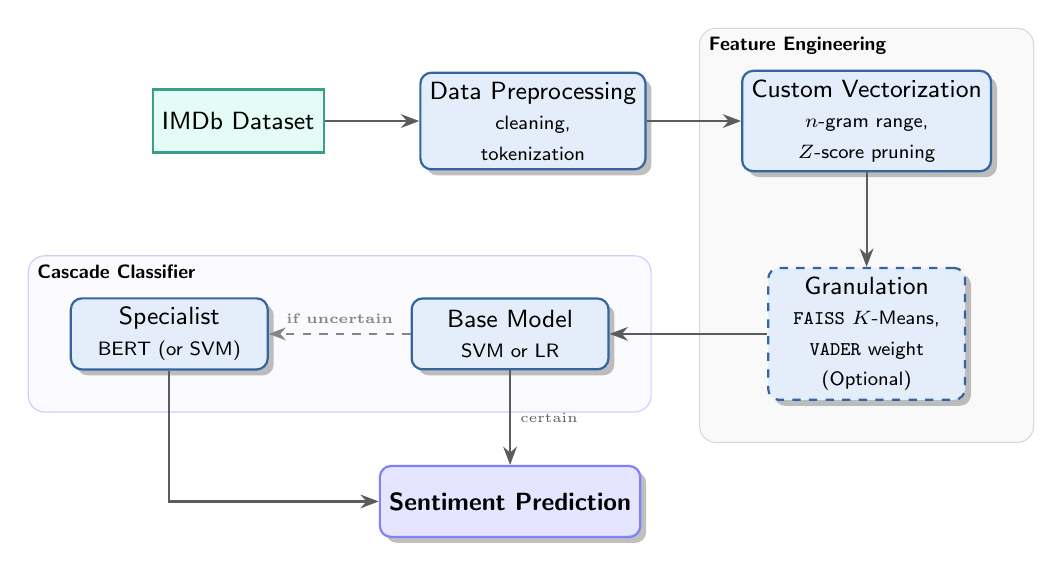
\begin{tikzpicture}[node distance=0.6cm and 1.2cm]
		
		% Row 1
		\node[datanode] (imdb) {IMDb Dataset};
		
		\node[stepnode, right=of imdb] (prep)
		{Data Preprocessing\\
			\scriptsize cleaning, \\
			\scriptsize tokenization };
		
		\node[stepnode, right=of prep] (vector)
		{Custom Vectorization\\
			\scriptsize $n$-gram range, \\
			\scriptsize $\zscore$-score pruning};
		
		% row 2
		\node[stepnode, below=1.2cm of vector, dashed] (gran)
		{Granulation\\
			\scriptsize \code{FAISS} $K$-Means,\\
			\scriptsize \code{VADER} weight \\
			\scriptsize (Optional)};
		
		\node[stepnode, left=2cm of gran] (base)
		{Base Model\\
			\scriptsize SVM or \logreg{}};
		
		\node[stepnode, left=1.8cm of base] (specialist)
		{Specialist\\
			\scriptsize BERT (or SVM)};
		
		% row 3
		\node[finalnode, below=1.2cm of base] (pred)
		{Sentiment Prediction};
		
		% Arrows
		\draw[arrow] (imdb)   -- (prep);
		\draw[arrow] (prep)   -- (vector);
		
		% Connection between Row 1 and Row 2
		\draw[arrow] (vector.south) -- (gran.north);
		
		\draw[arrow] (gran)   -- (base);
		
		% Cascade
		\draw[dasharrow] (base) -- (specialist) 
		node[midway, above, font=\tiny\bfseries] {if uncertain};
		
		% Output
		\draw[arrow] (base.south) -- (pred.north)
		node[midway, right, font=\tiny] {certain};
		
		% BERT to Prediction
		\draw[arrow] (specialist.south) |- (pred.west);
		
		% Background
		\begin{scope}[on background layer]
			% Feature Box
			\node[draw=gray!30, fill=gray!5, rounded corners=6pt, inner sep=15pt,
			fit=(vector) (gran)] (feBox) {};
			\node[font=\sffamily\bfseries\scriptsize, anchor=north west] at (feBox.north west) {Feature Engineering};
		\end{scope}
		
		\begin{scope}[on background layer]
			% Cascade Box
			\node[draw=blue!20, fill=blue!2, rounded corners=6pt, inner sep=15pt,
			fit=(base) (specialist)] (ccBox) {};
			\node[font=\sffamily\bfseries\scriptsize, anchor=north west] at (ccBox.north west) {Cascade Classifier};
		\end{scope}
		
	\end{tikzpicture}
	\caption{High-level pipeline of the cascade sentiment analysis system.}
	\label{fig:pipeline}
\end{figure*}



\subsection{Data Preprocessing} \label{sec:preprocessing}

While the original IMDb dataset is perfectly balanced and pre-divided into equal training and testing sets, this study merges both sets to perform data deduplication based on exact matches of the raw review text. This process identified and removed $418$ duplicate entries, resulting in a refined, unique dataset of \num{49582} reviews. The dataset is shuffled and re-divided into a training set of \num{24791} reviews (approx. $50\%$), a validation set of \num{17353} reviews (approx. $35\%$), and a testing set of \num{7438} reviews (approx. $15\%$). Stratification is employed to maintain a balanced distribution of positive and negative sentiments across all sets. The textual data is processed in parallel using a process pool executor. Each review is processed sequentially as follows:

\begin{enumerate}
	\item {Unicode normalization} converts the original text to Normalization Form Compatibility Composition (NFKC) form to ensure consistent character representation.
	
	\item {Typographical unification} uses a translation table to replace uncommon characters with their ASCII equivalents (e.g., \literal{\ldots} $\rightarrow$ \literal{...} or \literal{---} $\rightarrow$ \literal{-}).
	
   \item {Tag removal} replaces any substrings within the HTML tags \code{<>} with a space.
	
	\item {Whitespace condensation} collapses multiple whitespace characters into a single space, and strips leading/trailing spaces.
	
	\item {Contraction expansion} is implemented using \code{con\-tra\-ctions.fix} function to expand English contractions (e.g., \literal{don't} $\rightarrow$ \literal{do not}).
	
	\item {Tokenization} produces \code{tokens\_cased} using NLTK's \code{word\_tokenize}.
	
	\item {Lowercasing} converts each token in \code{tokens\_cased} to the lowercase form, resulting in \code{tokens\_lower}.
	
	\item {POS-filtered tokenization} replaces the standard stop-word removal (Sec.~\ref{sec:stop-word-removal}); the expanded text (\code{tokens\_\-lower}) is filtered based on the POS tags; the result is stored as \code{tokens\_filtered}.
	
	\item {Alphabetic filtering} removes any character that is not a letter (a-z, A-Z) from \code{tokens\_lower}; tokens that become empty after this removal are discarded. The result is \code{tokens\_letters}.
	
	\item {Stemming} produces \code{tokens\_stemmed} from \code{tokens\_lower} by applying the Porter stemmer.
	
	\item {Lemmatization} applies the WordNet lemmatizer to \code{tokens\_lower}, producing \code{tokens\_lemmatized}.
\end{enumerate}

After processing, each review is stored as a dictionary containing the various token representations. The dictionaries are then converted to Pandas DataFrames with a consistent column order and saved as Parquet files (\code{train.parquet}, \code{val.parquet}, \code{test.parquet}). This format enables selective loading of representations in subsequent experiments.

\subsubsection{Stop-Word Removal}
\label{sec:stop-word-removal}

During the POS-filtering step, the dimensionality of the $n$-gram feature space can be reduced by removing words that carry little sentiment value---commonly termed stop words. However, because this step is inherently subjective and risks discarding subtle contextual cues, the standard stop-word removal using the English stop-word list provided by scikit-learn's \code{CountVectorizer} is bypassed as that list contains words such as \literal{well}, whose presence may be informative (e.g., \literal{well filmed}). 

Instead, stop-word filtering is kept to a minimum by utilizing a custom POS-based approach. The approach relies on the tags assigned by the spaCy library: coarse-grained Universal POS (UPOS) tags\footnote{\url{https://universaldependencies.org/u/pos/}} and fine-grained Penn Treebank tags\footnote{\url{https://www.ling.upenn.edu/courses/Fall_2003/ling001/penn_treebank_pos.html}}. (To avoid computational overhead parser and Named Entity Recognizer (NER) of the SpaCy's English model are disabled.) 

The POS filtering removes tokens that satisfy any of three specific criteria:

\begin{itemize}
	\item {Auxiliary verbs (except modals)}: tokens with the coarse tag \postag{AUX} (auxiliary) are removed, unless their fine-grained tag is \postag{MD} (modal auxiliary). Thus, words such as \literal{is}, \literal{are}, \literal{was}, and \literal{have} are removed, while modals like \literal{can}, \literal{will}, and \literal{must} are retained.
	\item {Determiners}: tokens with the coarse tag \postag{DET} (determiner) are removed. Examples include \literal{a}, \literal{an}, \literal{the}, \literal{many}, and \literal{my}.
	\item {Possessive endings}: tokens with the fine-grained tag \postag{POS} (possessive ending) are removed. This typically corresponds to the possessive clitic \literal{'s}.
\end{itemize}

The application of these rules is demonstrated in Table~\ref{tab:pos-filtering}. The listed tags include basic parts of speech such as pronouns (\postag{PRON}/\postag{PRP}), verbs and auxiliaries (\postag{VERB}/\postag{VBN}, \postag{AUX}/\postag{VBP}), adverbs (\postag{ADV}/\postag{RB}), determiners (\postag{DET}/\postag{DT}, \postag{DET}/\postag{PRP\$}), adjectives (\postag{ADJ}/\postag{JJ}, \postag{ADJ}/\postag{JJR}), nouns (\postag{NOUN}/\postag{NN}, \postag{NOUN}/\postag{NNS}), adpositions (\postag{ADP}/\postag{IN}), and punctuation (\postag{PUNCT}/\postag{.}). Rows designated for removal are highlighted in \textbf{bold} to help visualize how the approach works.

\begin{table}[tbp]%[htbp]
	\centering
	\caption{Example of POS filtering. Tokens intended for removal are depicted in bold.}
	\label{tab:pos-filtering}
	\begin{tabular}{l l l l}
		\toprule
                      &               & \multicolumn{2}{c}{POS}\\ \cmidrule{3-4}
		Token         & Lowercased    & Coarse    & Fine-grained  \\ \midrule		
		I             & i             & PRON         & PRP              \\
		\textbf{have} & \textbf{have} & \textbf{AUX} & \textbf{VBP}     \\
		got           & got           & VERB         & VBN              \\
		myself        & myself        & PRON         & PRP              \\
		quite         & quite         & ADV          & RB               \\
		\textbf{a}    & \textbf{a}    & \textbf{DET} & \textbf{DT}      \\
		proud         & proud         & ADJ          & JJ               \\
		collection    & collection    & NOUN         & NN               \\
		with          & with          & ADP          & IN               \\
		\textbf{many} & \textbf{many} & \textbf{DET} & \textbf{DT}      \\
		more          & more          & ADJ          & JJR              \\
		titles        & titles        & NOUN         & NNS              \\
		on            & on            & ADP          & IN               \\
		\textbf{my}   & \textbf{my}   & \textbf{DET} & \textbf{PRP\$}   \\
		list          & list          & NOUN         & NN               \\
		!             & !             & PUNCT        & .                \\ \bottomrule
	\end{tabular}
\end{table}

\subsection{Feature engineering}

To evaluate the impact of vocabulary representation on model performance, the tokenized text is transformed into discrete feature spaces using combinations of unigrams, bigrams, and trigrams. However, higher-order $n$-grams naturally introduce massive, highly sparse feature spaces. To mitigate the curse of dimensionality, an attempt is made to employ a few dimensionality reduction techniques: custom vectorization, statistical pruning and semantic clustering.

\subsubsection{Custom Vectorization} \label{sec:custom_vec}

By default, scikit-learn's \code{CountVectorizer} removes terms listed in the \code{stop\_words} parameter, generates $n$-grams, and then prunes the vocabulary according to the \code{min\_df} and \code{max\_df} thresholds. To faithfully evaluate the various token representations produced during preprocessing, it is essential to preserve their exact structures. Therefore, the default tokenization behavior is overridden.

At this stage, each document is a list of tokens. The lists are joined into single, space-separated strings, and a custom \code{space\_tokenizer} is supplied to the vectorizer. This tokenizer bypasses the default regular-expression-based tokenizer and splits text strictly on spaces. The vectorizer is additionally configured with \code{lowercase=False} (lowercasing was already performed during preprocessing) and the desired \code{ngram\_range} (e.g., $(1,3)$). This customized pipeline ensures that scikit-learn's frequency-based pruning is applied directly to the finalized $n$-grams, effectively reducing dimensionality and promoting model generalization. For this study, the minimum document frequency is set to $10$ (\code{min\_df=10}) to discard extremely rare $n$-grams, and a maximum document frequency threshold of $70\%$ (\code{max\_df=0.7}) is established to filter out overly omnipresent combinations.

\subsubsection{Statistical Pruning} \label{sec:stat_pruning}

A custom statistical pruning method based on $\zscore$-scores is employed to discard neutral noise and retain only highly discriminative vocabulary. This process evaluates each feature by comparing its relative frequency between the positive class ($\positive$) and the negative class ($\negative$) through the following steps:

\paragraph{Smoothed Probabilities}

First, the smoothed token-level probability $\smoothedprob{\tokenclass}$ of a feature \ksremark{Czy jakoś oznaczamy tę cechę?} in a given class $\tokenclass$ is calculated. To prevent undefined logarithms resulting from zero-frequency occurrences, Laplace smoothing ($\smoothparam = 0.01$) is applied:
\begin{equation}
	\smoothedprob{\tokenclass} = \frac{\Count{\tokenclass} + \smoothparam}{\numbertokens{\tokenclass} + \smoothparam \vocabsize},
\end{equation}
where:
\begin{itemize}
	\item $\Count{\tokenclass}$ is the number of occurrences of the feature in class $\tokenclass$,
	\item $\numbertokens{\tokenclass}$ is the total number of tokens in all documents of class $\tokenclass$, and
	\item $\vocabsize$ stands for the total size of the vocabulary \ksremark{Czym jest vocabulary?}.
\end{itemize}
This formulation treats each feature as a token generator---representing the probability of drawing that specific term when sampling tokens from class $\tokenclass$.

\paragraph{Computing the ${\zscore}$-Score}
Next, the log-odds ratio of the feature's smoothed probability in the positive class $\smoothedprob{\positive}$ versus the negative class $\smoothedprob{\negative}$ is calculated. The $\zscore$-score normalizes this log-odds ratio by its standard error:
\begin{equation}
	\zscore = \frac{\ln\frac{\smoothedprob{\positive}}{\smoothedprob{\negative}}}{\sqrt{\frac{1}{\Count{\positive} + \smoothparam} + \frac{1}{\Count{\negative} + \smoothparam}}}.
	\label{eq:zscore}
\end{equation}

\paragraph{Thresholding}
Finally, features whose absolute $\zscore$-score falls below a defined threshold (e.g., $|\zscore| \le 2.0$ \ksremark{Skąd jest ta wartość?}) are discarded. This preserves only the vocabulary that demonstrates statistically significant separation in token distribution between the two classes.

\subsubsection{Semantic Clustering} \label{sec:semantic_clustering}

To address the sparsity inherent in BoW and TF-IDF representations, an optional clustering pipeline is implemented. Traditional static word embeddings such as Word2Vec are limited to individual words and cannot directly represent arbitrary multi-word $n$-grams. In contrast, transformer-based models like the one employed here---\texttt{all-MiniLM-L6-v2}---produce dense contextual embeddings of dimension 384 for any input text, including bigrams and trigrams. Although generating these embeddings is computationally expensive, they provide the most semantically rich representation currently available and were deliberately chosen to test whether powerful, context-aware grouping of $n$-grams can outperform simpler vocabulary reduction methods.

Each $n$-gram in the vocabulary is encoded with this Sentence Transformer model. The resulting embedding is then augmented with a sentiment score obtained from the VADER lexicon: the compound polarity score of the $n$-gram is multiplied by a tunable hyperparameter $\weightparam$ and concatenated to the embedding vector. After augmentation, $L_2$ normalization is reapplied to restore unit length, ensuring the final vector space balances semantic proximity with sentiment polarity.

FAISS-accelerated K-Means clustering is utilized on these normalized, sentiment-aware vectors to partition the vocabulary into $\kconcepts$ discrete groups. Each cluster forms a ``concept'' that aggregates semantically and sentimentally related $n$-grams. The resulting mapping from each original $n$-gram to its concept identifier is stored. Concept-level feature matrices are then constructed by summing the term-frequency counts of all $n$-grams belonging to the same concept for each document. This produces a dense $D \times \kconcepts$ matrix that compresses the original high-dimensional vocabulary while preserving discriminative information. Statistical pruning via $\zscore$-scores can be applied to these concept features in exactly the same manner as to the original units, further reducing dimensionality and focusing the representation on the most sentiment-bearing concepts.

\subsubsection{Models and Training} \label{sec:models}

The system employs both traditional classifiers and a distilled transformer model. All models are trained on the training set and tuned on the validation set; the chosen hyperparameters are those that maximise validation accuracy.

\paragraph{Traditional Baselines} \label{sec:trad_models}

A Support Vector Machine (SVM)  and Logistic Regression Model (\logreg) are employed as the computationally efficient baselines. Both are trained on the TF-IDF and BoW $n$-gram vectors produced by the feature engineering pipeline. Both models are fitted on the same training split and evaluated on the same validation and test sets. The training utilizes the \code{scikit-learn} implementations with the following settings:

For the support vector machine, %This model minimizes the squared hinge loss with $L_2$ regularization. 
the default penalty $C=1.0$ is retained  and the solver’s iteration limit is set to $10{,}000$ to ensure convergence on high-dimensional data. Because the final cascade architecture requires calibrated probabilities, a Platt scaling calibrator (\texttt{CalibratedClassifierCV}) is wrapped around the SVM. This post‑processing step maps the decision values to $[0,1]$, producing approximate posterior probabilities for the positive class. Two kernel types are employed: a linear kernel and the Radial Basis Function (RBF) kernel, also known as the Gaussian kernel.

Logistic Regression Model directly models $\probLarge{}{\inputtext}$ by minimizing the log-loss (cross-entropy) with an $L_2$ penalty. It is configured with the \code{L-BFGS} solver, $C=1.0$, and a maximum of $1{,}000$ iterations. Unlike the SVM, \logreg{} natively outputs probability estimates without an external calibration step.

\paragraph{Deep Learning Model} \label{sec:distilbert_model}

The specific checkpoint \code{dis\-til\-bert-\-base-\-un\-ca\-sed-\-fi\-ne\-tu\-ned-sst-2-english} of DistilBERT is obtained from the Hugging Face hub; it has been pre-trained on large English corpora and already fine-tuned on the Stanford Sentiment Treebank (SST-2).

In this study, the model is further fine-tuned on the full IMDb training set. Input texts were cleaned (\code{text\_clean}) and subsequently tokenized with the DistilBERT tokenizer, and finally truncated or padded to a maximum length of $256$ tokens. Training is performed for $3$ epochs with a batch size of $16$, using the Adam optimizer with a learning rate of $2 \times 10^{-5}$. Mixed-precision (\code{float16}) computation is utilized to reduce memory consumption and accelerate training. Early stopping monitors the validation loss (patience $2$ epochs), and a learning rate reduction on plateau (factor $0.5$, patience $1$) is applied. A stratified $20\%$ hold-out from the training set serves as the validation partition. After training, the model outputs class probabilities through a softmax over the two logits.

\subsubsection{Configuration Enumeration}
\label{sec:config_enum}

The feature-engineering options define a large design space---token representations, $n$-gram ranges, pruning thresholds, clustering granularities, and sentiment weights. To populate this space with trained classifiers, every combination of the following axes is enumerated and evaluated on the validation set:

\begin{itemize}
	\item {Token representation:} Cased, lowered, letter-only, filtered, stemmed, and lemmatized.
	\item {$n$-gram range:} $(1,1)$, $(1,2)$, $(1,3)$. The default $(1,3)$ is used for the full combinatorial sweep; narrower ranges are tested in the vocabulary-depth test.
	\item {$\zscore$-score threshold:} $0,1,2,3,4$, where $0$ disables pruning.
	\item {Concept granularity ($k$):} $0$ (no clustering), $500$, $5\,000$, $10\,000$.
	\item {Sentiment weight ($\weightparam$):} $0$, $1$, $10$, applied to the VADER score when augmenting embeddings.
	\item {Vectorisation type:} BoW and TF-IDF (custom implementations).
	\item {Classifier:} linear SVM (with Platt scaling) and \logreg{}. Note that RBF SVM is tested in Section~\ref{sec:Impact-of-Kernel}, but it proved to be much slower with no accuracy benefit.
\end{itemize}
Not all combinations are independent: for example; when $\kconcepts=0$ the sentiment weight is irrelevant. For every configuration, the model is trained on the training set and its raw prediction vectors and classification reports are saved to disk. At this stage no representation is selected; the pool of candidate classifiers is merely created for subsequent cascade-oriented analysis. 

\subsection{Cascade Ensemble} \label{sec:cascade}

To balance the computational efficiency of traditional machine learning algorithms with the deep understanding capacity of transformer-based models, a cascade ensemble architecture is proposed. The design follows the 3WD paradigm, where each instance is assigned to one of three regions based on the predictive confidence of a lightweight base model. Instances classified with high confidence are accepted immediately, while those falling into a boundary region of uncertainty are deferred to a specialist.

\subsubsection{Architecture} \label{sec:cascade_architecture}

The cascade operates in three stages:

\begin{enumerate}
	\item {Initial inference:} A computationally inexpensive base model evaluates an input text $\inputtext$ and outputs a probability score
	\begin{equation}
		\probSmall{\mBase} = \probLarge{\mBase}{\inputtext} \in [0,1].
	\end{equation}
	
	\item {Uncertainty delegation:} A threshold $\thresh \in [0, 0.5]$ is defined. The intervals $[0, \thresh)$ and $(1-\thresh, 1]$ correspond to high-confidence negative and positive predictions, respectively, which are accepted without further processing. Otherwise $\inputtext$ is placed in the boundary region if the base model's probability lies within the closed interval:
	\begin{equation}
		\thresh \le \probSmall{\mBase} \le 1 - \thresh,
	\end{equation}
	
	\item {Specialist resolution:} Instances in the boundary region are forwarded to a specialist model. Three specialist configurations are evaluated:
	\begin{itemize}
		\item a generic DistilBERT classifier used as a black-box specialist;
		\item a DistilBERT specialist fine-tuned exclusively on the boundary samples mined from the validation set;
		\item an SVM specialist trained on the same boundary samples to verify whether a two-stage traditional approach would achieve satisfying results.
	\end{itemize}
\end{enumerate}

\begin{figure*}[tbp]
	\centering
	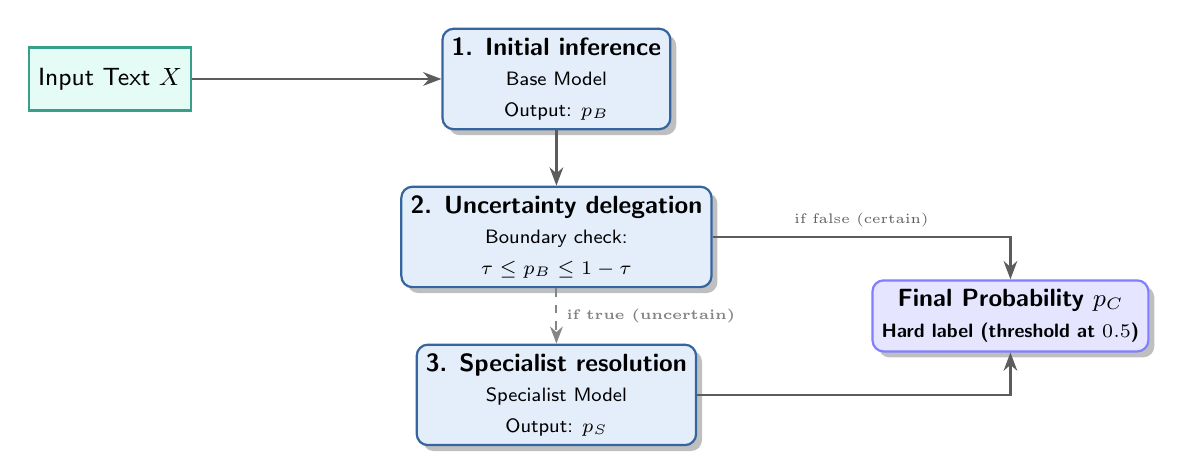
\begin{tikzpicture}[node distance=2em and 9em]
		
		% Nodes
		% Left side: input
		\node[datanode] (input) {Input Text $\inputtext$};
		
		% Middle column: cascade
		\node[stepnode, right=of input] (base)
		{\textbf{1. Initial inference}\\
			\scriptsize Base Model\\
			\scriptsize Output: $\probSmall{\mBase}$};
		
		\node[stepnode, below=of base] (delegation)
		{\textbf{2. Uncertainty delegation}\\
			\scriptsize Boundary check:\\
			\scriptsize $\thresh \le \probSmall{\mBase} \le 1 - \thresh$};
		
		\node[stepnode, below=of delegation] (specialist)
		{\textbf{3. Specialist resolution}\\
			\scriptsize Specialist Model\\
			\scriptsize Output: $\probSmall{\mSpec}$};
		
		% Right side: output
		\path (delegation) -- (specialist) coordinate[midway] (mid_del_spec);
		\node[finalnode, right=4cm of mid_del_spec] (pred) 
		{Final Probability $\probSmall{\mCas}$\\
			\scriptsize Hard label (threshold at $0.5$)};
		
		% Arrows
		% Input to base
		\draw[arrow] (input) -- (base);
		
		% Base to delegation
		\draw[arrow] (base) -- (delegation);
		
		% delegation to specialist
		\draw[dasharrow] (delegation) -- (specialist) 
		node[midway, right, font=\tiny\bfseries] {if true (uncertain)};
		
		% delegation to output
		\draw[arrow] (delegation.east) -| (pred.north) 
		node[pos=0.25, above, font=\tiny] {if false (certain)};
		
		% specialist to output
		\draw[arrow] (specialist.east) -| (pred.south);
		
	\end{tikzpicture}
	\caption{Architecture of the three-stage cascade showing initial inference, uncertainty delegation, and specialist resolution.}
	\label{fig:cascade_architecture_diagram}
\end{figure*}

Let $\probSmall{\mSpec} = \probLarge{\mSpec}{\inputtext}$ denote the probability output of the chosen specialist. The final cascaded probability, $\probSmall{\mCas}$, is obtained by combining the two models:
\begin{equation}
	\probSmall{\mCas} = \probLarge{\mCas}{\inputtext} =
	\begin{cases} 
		\probSmall{\mSpec}, & \probSmall{\mBase} \in [\thresh, 1 - \thresh], \\[4pt]
		\probSmall{\mBase}, & \probSmall{\mBase} \notin [\thresh, 1 - \thresh].
	\end{cases}
\end{equation}

The hard class label is derived by thresholding $\probSmall{\mCas}$ at $0.5$: values strictly greater than $0.5$ are taken as positive, otherwise negative.

\subsubsection{Threshold Selection} \label{sec:threshold_selection}

The delegation threshold $\thresh$ governs the trade-off between the fraction of instances processed by the base model $\mBase$ (coverage) and the overall performance of the hybrid system (global accuracy). To determine both the optimal base model $\mBase_{\!\optimal}$ and the optimal threshold $\thresh_{\!\optimal}$, a joint sweep is performed on the validation set. For every candidate base model $\modelvar$ obtained from the configuration enumeration and for every candidate threshold $\sweepthresh \in [0,0.5]$, the cascade is simulated using the generic DistilBERT. The hybrid accuracy $\hybridacc{\modelvar}{\sweepthresh}$ is computed as defined below, and the pair $(\modelvar,\sweepthresh)$ that maximizes this metric is selected. Let the validation set contain $\numVal$ instances, indexed by $\idx = 1,\dots,\numVal$. For a fixed candidate base model $\modelvar$, denote the predicted probability for instance $\idx$ by $\probSmall{\mBase_{\!\modelvar}}^{(\idx)}$. For a candidate threshold $\sweepthresh$, the acceptance mask for instance $\idx$ under model $\modelvar$ is:
\begin{equation}
	\accMask{\modelvar}{\idx}{\sweepthresh} = \mathbf{1}\bigl[ \baseProb{\modelvar}{\idx} \le \sweepthresh \;\lor\; \baseProb{\modelvar}{\idx} \ge 1-\sweepthresh \bigr].
\end{equation}
The coverage of model $\modelvar$ at threshold $\sweepthresh$ is the fraction of instances it accepts:
\begin{equation}	
	\coverage{\modelvar}{\sweepthresh} = \frac{1}{\numVal}\sum_{\idx=1}^{\numVal} A_{\modelvar,\idx}(\sweepthresh).
\end{equation}
The hybrid accuracy of the cascade when using model $\mu$ and threshold $\sweepthresh$ is:
\begin{equation}
	\hybridacc{\modelvar}{\sweepthresh} = \frac{1}{\numVal}\sum_{\idx=1}^{\numVal} \mathbf{1}\bigl[ \cascadePred{\modelvar}{\idx}{\sweepthresh} = \predVal_{\idx} \bigr].
\end{equation}
where $\hat{y}_{\iota}^{\,\mCas}(\sweepthresh)$ is the cascade's final prediction for instance $\iota$ under the given model and threshold. The optimal base model and the optimal threshold are chosen simultaneously:
\begin{equation}
	(\mBase_{\!\optimal},\;\thresh_{\!\optimal}) =
	\arg\max_{\mu,\;\sweepthresh \in [0,0.5]}
	\aleph(\mu,\sweepthresh).
\end{equation}

\subsubsection{Specialist Training} \label{sec:specialist_training}

Two types of specialists are trained exclusively on the validation documents whose base model prediction probability $\probSmall{\mBase}^{(\idx)}$ falls within $[\thresh, 1-\thresh]$.

\subparagraph{Specialist SVM.} The same SVM architecture and hyperparameters as the base model is employed, but the model is fitted solely on the TF-IDF representations of the boundary samples. This yields a lightweight specialist that shares the feature space and decision function type of the base model while concentrating on the ambiguous region.

\subparagraph{Specialist BERT.} The basic DistilBERT model is further fine-tuned on the boundary subset. The backbone is partially frozen: the first $5$ transformer layers are kept frozen, while the remaining layers and the classification head remain trainable. The specialist is trained for $10$ epochs with a lower learning rate of \num{2e-6}, batch size $16$, and early stopping (patience $3$ epochs). All other training settings (mixed precision, tokenizer, maximum sequence length) are identical to the basic fine-tuning. This procedure encourages the model to specialize in the ambiguous region of the decision boundary without over-fitting to the relatively small hard-sample set.

\subsection{Implementation}

All experiments, data transformations, and statistical analyses are implemented in Python. The architecture leverages open-source libraries across the different domains of the experimental pipeline:

\begin{itemize}
	\item {Data Management and Processing:} Core data manipulation, matrix operations, and dataset parsing are handled using \code{pandas} and \code{NumPy}.
	
	\item {Natural Language Processing:} the \code{contractions} library is utilized alongside \code{NLTK}, which provides the implementations for Porter Stemming and WordNet Lemmatization. Context-aware POS filtering is executed with \code{spaCy} (\texttt{en\_core\_web\_sm}). Lexicon-based sentiment scoring is provided by \code{vaderSentiment}.
	
	\item {Classical Machine Learning:} the construction of BoW and TF-IDF matrices, as well as the implementation of the traditional classifiers (linear SVM and \logreg), are conducted using \code{scikit-learn}. For high-dimensional semantic clustering, \code{FAISS} is employed to perform GPU-accelerated K-Means clustering.
	
	\item {Deep Learning:} the deep learning components of the cascade architecture are built upon the \code{TensorFlow} and \code{Keras} frameworks. The DistilBERT model and its tokenizer are sourced from the Hugging Face \code{transformers} library. The generation of dense semantic vectors prior to clustering is powered by the \code{sentence-transformers} library.
	
	\item {Statistical Testing and Visualization:} \code{statsmodels} is employed to perform McNemar's tests. All graphical representations are generated with \code{matplotlib}, \code{seaborn}, and the \code{wordcloud} library.
\end{itemize}

The code can be found in the repository\footnote{\url{https://github.com/JanSupierz/Sentiment}}.
The main experiment is located in the \code{Experiment.ipynb} file, while the reusable structural components are in the \code{src/} directory, which contains the implementations of machine learning models, feature extraction methods, and utilities.
In the \code{scripts/} directory, all steps that appear in the notebook are available as standalone scripts; these files are intended mostly for one‑time use.
\section{Experiments} \label{chap:experiments}

\subsection{Datasets}

For the empirical evaluation in this study, the Large Movie Review Dataset is used---commonly referred to as the IMDb sentiment dataset \cite{Maas2011imdb}\footnote{\url{https://ai.stanford.edu/~amaas/data/sentiment/}}. This dataset serves as a standard benchmark for binary sentiment classification in natural language processing. It contains a total of \num{50000} highly polar movie reviews. The acquisition of the IMDb dataset is facilitated by TensorFlow Datasets (TFDS).

\subsubsection{Examples}

Below are example reviews from the dataset. These examples demonstrate the text's typical length, as well as its informal and rather descriptive style.

\paragraph{Label: Positive}

\begin{quote}	
	Wasn't sure what to expect from this film. I love watching Brosnan in any movie, he's always good, but this was totally different. He's a mess, and plays being a mess very well. In fact he reminded me of myself a few times back in uni :) So yes, there's not a lot of violence, there's not a lot of action, but the dialogue is cracking, the acting is superb and very refreshing, and it's pretty funny too :) I don't think you'll come out of the cinema going "Wow! I was blown away", but you'll come out smiling having enjoyed a good film. Can't ask for more than that.<br /><br />Oh, and if you're lucky, some moron will put the adverts reel in wrong and you'll get inverted, upside down, reversed (with reversed audio) adverts!! Brilliant. Nothing like watching a Jack Daniels ad where the drink goes back into the bottle from the glass with a gruff American "Twin Peaks" commentary :)
\end{quote}

At first sight, the positive text tends to use words with positive connotations---such as \literal{love}, \literal{good}, and \literal{lucky}---as well as emoticons like \literal{:)}. However, clearly negative words (\literal{mess} or \literal{moron}) can also be found, demonstrating that context is crucial.

\paragraph{Label: Negative}

\begin{quote}	
	The first half of the movie is not that bad actually. Although there's not really too much depth in the characters, the story is somehow funny and generally OK with potential to get better, which it doesn't.<br /><br />In the second half things start to turn for the worse, not only for the characters in the movie, but also for the viewer, who will be basically waiting for the story to come to its obvious end.<br /><br />The previous user comment mentioned: "It's a love story, a road movie, a thriller, a comedy of errors, an 80's movie and most of all, it's a Jonathan Demme movie."<br /><br />Well, please allow me to rephrase that: "It's a boy gets girl story, they happen to be driving around in cars, the thrill is gone as it is all too clear how things will evolve, there wasn't any scene in this film to which one might laugh out loud, it does have some slight 80's feeling and yes, Jonathan Demme really was the director."
\end{quote}

The negative review shows how sentiment can shift within a single text. The author begins with positive evaluations, using phrases conceding that the film is \literal{not that bad.}. The tone progressively deteriorates, relying on phrases that express disappointment such as \literal{turn for the worse} and \literal{the thrill is gone.}. Furthermore, sarcasm and cynicism play a crucial role in cementing the overall negative polarity.

\paragraph{Possibly Mislabeled}

\begin{quote}
	I first watched Kindred in 1987 along with another movie called devouring waves. I remember back then i hated them both and i have never really bothered to watch them again.<br /><br />However i have recently started a crusade to collect as many 80's horror titles in their original boxed form, That have been deleted for some time. I have got myself quite a proud collection with many more titles on my list!<br /><br />The Kindred although i have not as yet got a copy is high priority as all the old movies i didn't like back then, I now own and have now re-watched and think they are brilliant and the bits i do remember of the Kindred are now driving me to want to get hold of a copy A.S.A.P.<br /><br />Hurray for the 80's and long live horror!
\end{quote}

The text is labeled as negative within the dataset, but is overly positive. This discrepancy suggests that either the entire message is meant to be read as sarcastic, or the user made an error when selecting their rating.

\subsection{Methodology} \label{sec:methodology}

The aim is to define the impact of each individual step in the pipeline described in Chapter~\ref{sec:our-approach} and to determine if a cascade system further improves upon those results. To do so, two experiments, \textbf{Experimental Evaluation Sequence} (Sec.~\ref{sec:ExperimentalEvalSeq}) and \textbf{Cascade System Experiment} (Sec.~\ref{sec:CascadeSysExp}), are constructed. Both experiments consist of sub-stages where the configuration that yields the highest validation metric is considered the best setting and is adopted as the baseline for the next stage. The test set is never used until the final cascade evaluation. The experiments are outlined in the next sections.

\subsubsection{Experimental Evaluation Sequence} \label{sec:ExperimentalEvalSeq}

The enumeration space defined in Section~\ref{sec:config_enum} is explored through a series of sub-experiments on the validation set. Each step refines the process and provides insights into its individual impact on the overall pipeline. Ultimately, the best standalone model is identified---this model is not necessarily selected for the cascade system, as peak standalone performance may not translate to optimal combined performance. The predictions from all intermediate models during this phase are used to simulate the cascade in the subsequent experiment detailed in Section~\ref{sec:CascadeSysExp}.

\begin{enumerate}
	\item \textbf{Preprocessing and basic representation.} Using the default \texttt{CountVectorizer} with $(1,3)$ $n$-grams, the four combinations of text variant (clean vs.\ expanded) and casing (cased vs.\ lowercased) are evaluated with both BoW and TF-IDF for the linear SVM and \logreg{}. This stage identifies the best preprocessing choice (expanded, lowercased, TF-IDF).
	
	\item \textbf{Custom vectorization and $\mathbf{\zscore}$-score pruning.} All six token representations (cased, lower, letters, filtered, stemmed, lemmatized) are combined with $\zscore$-score thresholds $\zscore \in \{0,1,2,3,4\}$ and both BoW and TF-IDF, using the custom space-tokenizer described in Section~\ref{sec:custom_vec}. The best token representation and pruning level are chosen for each model.
	
	\item \textbf{Vocabulary depth ($\boldsymbol{n}$-gram range).} With the best token representation and $\zscore=2.0$ fixed, the $n$-gram range is varied from $(1,1)$ to $(1,3)$. This test measures the trade-off between accuracy and feature-space size.
	
	\item \textbf{Kernel type.} With the same settings as in the previous step, the impact of the kernel is assessed. The accuracy and training times of SVMs with a linear kernel and an RBF kernel are compared at two \code{max\_iter} limits: \num{1000} and \num{10000}.
	
	\item \textbf{Semantic clustering.} For $\kconcepts \in \{\num{500}, \num{5000}, \num{10000}\}$ and sentiment weights $\weightparam \in \{0, 1, 10\}$, concept matrices are built from the optimal unit features (Section~\ref{sec:semantic_clustering}) and evaluated with both SVM and \logreg. This gauges whether concept compression can match the unclustered baseline.
	
	\item \textbf{Cascade threshold sweep.} For every candidate base model from the configuration enumeration (Section \ref{sec:config_enum}), a sweep over $\thresh \in [0,0.5]$ is performed on the validation set, simulating the cascade. The pair (base model, $\thresh$) that maximizes the hybrid accuracy is selected, and identifying the optimal base model (Section~\ref{sec:threshold_selection}).
\end{enumerate}

\subsubsection{Cascade System Experiment} \label{sec:CascadeSysExp}

The cascade architecture depends on the assumption that the base model's predictive confidence correlates with correctness, so that delegating uncertain instances to a specialist can improve overall performance. The experiments in this subsection first validate this confidence assumption. Then, three alternative specialist strategies are compared to determine whether a computationally heavy model is required, or whether the same model type trained on the boundary region is sufficient.

%\paragraph{Confidence Analysis}

To verify that the delegation threshold $\thresh$ genuinely isolates difficult cases, the base model's predicted probabilities are binned and the empirical accuracy in each bin is examined. For instances with probabilities close to $0$ or $1$ (the acceptance regions), the observed accuracy and coverage should be substantially higher than for instances with probabilities near $0.5$ (the boundary region) to confirm that the interval $[\thresh,\,1-\thresh]$ captures cases where the base model is most error-prone.

%\paragraph{Specialist Comparison}

Three cascade variants are evaluated to assess which specialist configuration yields the best performance. The base model is fixed to the optimal linear SVM identified by the sweep (Section~\ref{sec:threshold_selection}), and the delegation threshold is set to $\thresh = 0.254$ (Section~\ref{sec:threshold_selection}). Three specialist variants are tested:

\begin{itemize}
	\item \textbf{Base DistilBERT}: the generic DistilBERT model (Section~\ref{sec:distilbert_model}).
	\item \textbf{SVM specialist}: the linear SVM introduced in Section~\ref{sec:specialist_training}.
	\item \textbf{BERT specialist}: the fine-tuned DistilBERT described in Section~\ref{sec:specialist_training}.
\end{itemize}

All three cascade variants are evaluated on the held-out test set, together with the standalone base SVM and the standalone DistilBERT baseline. The final cascade prediction follows the combination rule defined in Section~\ref{sec:cascade_architecture}: the base model's output is used for instances outside the boundary region, and the specialist's output is used for instances inside it.

\subsection{Evaluation Metrics}

Because the data splits are exactly balanced through stratified sampling, accuracy $\accuracy$ and macro $\FOne$-score are equally reliable indicators of performance. 
Both are reported in all experiments. The primary metric for selecting the best configuration is accuracy $\accuracy$, as it directly aligns with the McNemar test.

\subsubsection{Notation}
Let $\numVal$ be the number of test instances. For each instance $\idx \in \{1,\dots,\numVal\}$, let $\predVal_{\idx} \in \{0,1\}$ denote the true label and $\hat{\predVal}_{\idx} \in \{0,1\}$ the predicted label.

Accuracy $\accuracy$ is the fraction of correct predictions:
\begin{equation}
	\accuracy = \frac{1}{\numVal} \sum_{\idx=1}^{\numVal} \mathbf{1}[\hat{\predVal}_{\idx} = \predVal_{\idx}],
\label{eq:accuracy}
\end{equation}
where $\mathbf{1}[a]$ equals 1 if condition $a$ is true, otherwise it is 0.

In the following sections, we use the notation taken from \citep{id:Siminski2021Outlier}.
The first item in a pair describes the original class (positive $\positiveclass$ or negative $\negativeclass$). 
The second item -- the elaborated class by classifiers, eg.
$\ksTP$ stands for the number of positive class items classified as positive (true positive), 
$\ksOriginalPositive$ is the number of positive items in a dataset,
$\ksPredictedPositive$ is the number of items classified as positive,
and $\ksAll$ stands for the number of all items.

Macro $\FOne$-score averages the $\FOne$-score over the two classes without weighting.
For a given class $\instanceClass \in \{0,1\}$, let $\TP\insclass = \ksTP\insclass$, $\FP\insclass = \ksFP\insclass$, $\FN\insclass = \ksFN\insclass$ be the true positives, false positives, and false negatives, respectively.
The per‑class precision, recall, and $F_1$ are:
\begin{equation}	
   \precision\insclass = 	\frac{\text{TP}\insclass}{\text{TP}\insclass + \text{FP}\insclass} = \frac{\ksTP\insclass}{\ksPredictedPositive\insclass},
\end{equation}
%
\begin{equation}
   \recall\insclass = \frac{\text{TP}\insclass}{\text{TP}\insclass + \text{FN}\insclass} = \frac{\ksTP\insclass}{\ksOriginalPositive\insclass},
\end{equation}
%
\begin{equation}
   \FOne\insclass = \frac{2P\insclass  R\insclass}{P\insclass + R\insclass} =  \frac{2\ksTP\insclass}{\ksOriginalPositive\insclass + \ksPredictedPositive\insclass}.
\end{equation}
%
The macro $\FOne$-score $\MacroFOne$ is the arithmetic mean of the two per‑class values:
\begin{equation}
	\MacroFOne = \frac{1}{2} \sum_{\instanceClass=0}^{1} \FOne\insclass.
	\label{eq:macro:f1}
\end{equation}

\subsubsection{Statistical Significance Testing}

All pairwise model comparisons are validated with McNemar’s test at the $\mcnemarp = 0.05$ significance level.
The test evaluates whether the error distributions of two classifiers, computed on the same set of instances, differ significantly.
In each experiment a baseline is chosen---typically the best‑performing configuration from the previous stage.
The implementation follows \texttt{statsmodels}, using the $\chi^2$ approximation with a continuity correction (\code{exact=False}, \code{correction=True}).
Raw $\mcnemarp$-values are reported without multiplicity correction, given the sequential, hypothesis‑driven design.

Let $\missclassified{10}$ be the number of instances misclassified by the baseline only, and $\missclassified{01}$ the number misclassified by the challenger only.
The null hypothesis is $\nullhypo: \missclassified{10} = \missclassified{01}$ (the two classifiers have the same error distribution).
The test statistic is:
\begin{equation}
	\mcnemarchi = \frac{(|\missclassified{10} - \missclassified{01}| - 1)^2}{\missclassified{10} + \missclassified{01}},
\end{equation}
which, under $\nullhypo$, approximately follows the $\mcnemarchi$ distribution with one degree of freedom.

The $\mcnemarp$-value is the probability that a $\mcnemarchi_1$ random variable would be at least as large as the observed value $\mcnemarchi_{\text{obs}}$. \ksremark{Czy tu nie będzie konfliktu oznaczeń? $\chi^2_1$ ma 1 stopień swobody, a $\chi^2_{\text{obs}}$ to obserwowane? Może $\hat{\chi}^2_1$ jako obs?}
In the code, this is computed via the survival function: \code{stats.chi2.sf(}$\mcnemarchi$\code{, df=1)}.
If $\mcnemarp < 0.05$, the difference between the two classifiers is considered statistically significant.
Because the statistic squares the absolute difference, the test is two‑sided: it detects any deviation from $\nullhypo$, irrespective of increase or decrease in the accuracy.

\subsubsection{Visualization of Statistical Significance}

Every figure and table consistently encodes the outcome of McNemar’s test:

\begin{itemize}
	\item \textbf{Graphs.} Significant comparisons ($p < 0.05$) are drawn with full colour saturation, thick lines, and solid markers; non‑significant ones use low opacity, thinner lines, and hollow markers. The legend carries the tags “Sig.\ Diff” and “Not Sig.” where appropriate.
	\item \textbf{Tabular reports.} Rows with $p < 0.05$ are set in bold and accompanied, when a significant result is obtained, a directional arrow ($\uparrow$ for improvement, $\downarrow$ for degradation) is added based on the raw accuracy difference. The baseline row is also bold. Rows with $p \ge 0.05$ use regular weight and no arrow, as illustrated in Table~\ref{tab:McNemarExample}.
\end{itemize}

\begin{table}[htbp]
	\centering
	\caption{Example results of the McNemar test. Bold text indicates statistical significance, while directional arrows denote a significant increase or decrease in accuracy of the challenger model relative to the baseline.}
	\label{tab:McNemarExample}
	\begin{tabular}{llcr}
		\toprule
		Model Description & $\accuracy$ &  $\uparrow$/$\downarrow$ & $\mcnemarp$-value \\
		\midrule
		\textbf{Challenger A} & \textbf{0.8542} & \textbf{$\uparrow$} & \textbf{0.001} \\
		\textbf{Baseline model}                      & \textbf{0.8310} &                      & \textbf{---}  \\
		\textbf{Challenger B}  & \textbf{0.8103} & \textbf{$\downarrow$} & \textbf{0.023} \\
		Challenger C                 & 0.8325          &                      & 0.412 \\
		\bottomrule
	\end{tabular}
\end{table}

\subsection{Results}
\label{sec:results}

This section presents the evaluation of linear SVM and \logreg{} classifiers across various configurations. Initial tests establish that linear SVMs consistently outperform \logreg{} models, with TF-IDF representations universally yielding superior predictive performance compared to standard BoW. The findings demonstrate that implementing statistical pruning effectively mitigates the dimensionality explosion associated with complex $n$-grams while preserving optimal classification accuracy. Ultimately, the results validate the proposed cascade ensemble methodology; delegating uncertain predictions from a highly efficient linear base model to a deep-semantic BERT specialist resolves non-linear contextual cues, achieving a peak combined macro $F_1$-score of approximately $92.3\%$ and significantly outperforming standalone baselines.

The analysis is split into several stages, each describing an individual impact:

\begin{enumerate}
	\item \textbf{Experimental Evaluation Sequence:}
	\begin{itemize}
		\item \nameref{sec:Impact-of-Casing-and-Text-Expansion} (Sec.~\ref{sec:Impact-of-Casing-and-Text-Expansion})
		\item \nameref{sec:Impact-of-Filtering} (Sec.~\ref{sec:Impact-of-Filtering})
		\item \nameref{sec:Impact-of-Custom-Vectorization} (Sec.~\ref{sec:Impact-of-Custom-Vectorization})
		\item \nameref{sec:Impact-of-Vocabulary-Depth} (Sec.~\ref{sec:Impact-of-Vocabulary-Depth})
		\item \nameref{sec:Impact-of-Kernel} (Sec.~\ref{sec:Impact-of-Kernel})
		\item \nameref{sec:Impact-of-Semantic-Clustering} (Sec.~\ref{sec:Impact-of-Semantic-Clustering})
	\end{itemize}
	
	\item \textbf{Cascade System Experiment:}
	\begin{itemize}
		\item \nameref{sec:Impact-of-Certainty} (Sec.~\ref{sec:Impact-of-Certainty})
		\item \nameref{sec:Impact-of-Cascade-Ensemble} (Sec.~\ref{sec:Impact-of-Cascade-Ensemble})
	\end{itemize}
\end{enumerate}


\subsubsection{Impact of Casing and Text Expansion}
\label{sec:Impact-of-Casing-and-Text-Expansion}

In this test, the performance of two classical classifiers---linear SVM and \logreg{}---is evaluated across varying preprocessing and feature representation configurations. All models were trained on the training set. The evaluation metrics (macro $F_1$-score and accuracy) are computed on the validation set. The experimental conditions are categorized as follows:
\begin{itemize}
	\item Minimal preprocessing (Clean) vs. Contraction expansion (Expanded),
	\item Original capitalization (Cased) vs. Lowercased (Lower),
	\item BoW vs. TF-IDF (\code{ngram\_range=(1,3)}, \code{min\_df=10}, \code{max\_df=0.7}).
\end{itemize}

\begin{figure*}[tbp]
	\centering
	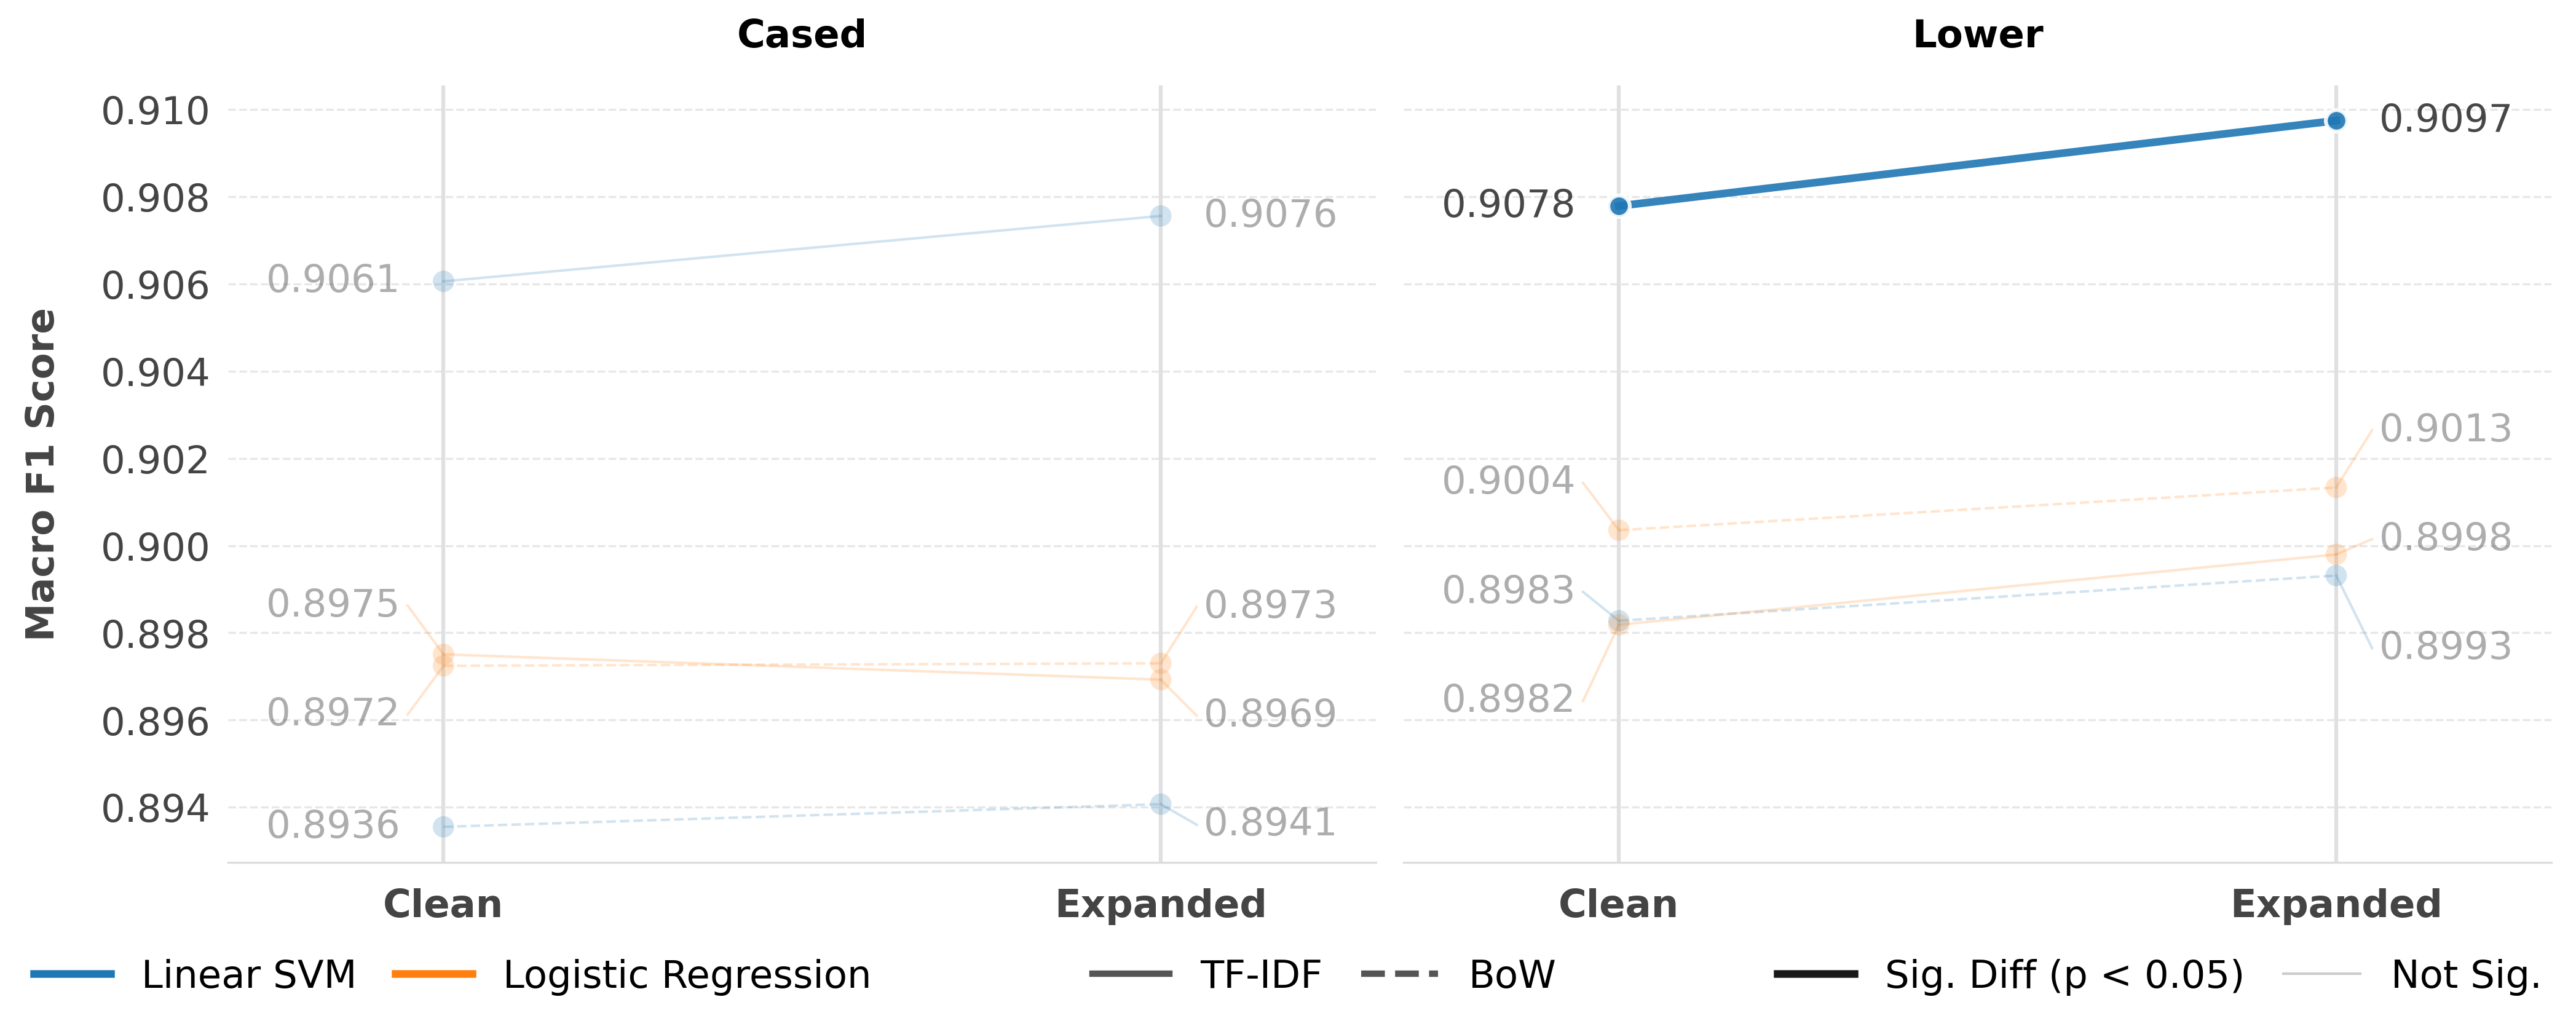
\includegraphics[width=\textwidth]{./figures/analysis/casing-effect-slopegraph.png}
	\caption{Macro $F_1$-scores comparing clean versus expanded text. The left and right panels display results for cased and lowercased text, respectively. Line colors differentiate the machine learning models (blue for Linear SVM, orange for Logistic Regression), while line styles denote the text representation (solid for TF-IDF, dashed for BoW). Full line opacity indicates a statistically significant difference ($\mcnemarp < 0.05$), with faded lines denoting insignificant changes. Only the lowercased Linear SVM utilizing TF-IDF demonstrated a significant performance impact upon expansion.}
	\label{fig:casing-expansion-effect}
\end{figure*}

As illustrated in Figure~\ref{fig:casing-expansion-effect}, the transition from cleaned to expanded text provides a statistically significant benefit for lower-cased text, as demonstrated by McNemar's test applied to the pairwise predictions. Other transitions are not found to be statistically significant and are thus grayed out on the graph.

%\paragraph{Comparative Analysis of Configurations}

Tables~\ref{tab:McNemarE1a} through \ref{tab:McNemarE1d} provide a cross-configuration analysis, comparing various models and representations against selected baselines. The first two tables use SVMs as the baseline models, and the latter two use \logreg{}. From these results, several key trends emerge:

\begin{enumerate}
	\item \textbf{Model Impact:} linear SVM consistently outperforms \logreg{} models across all equivalent settings.
	
	\item \textbf{Representation Impact:} TF-IDF features yield better performance than BoW.
\end{enumerate}


\begin{table*}[tbp]%[htbp]
	\centering
	\caption{McNemar test results analyzing the impact of casing, text expansion, representation, and model choice. Across all subtables, bold text indicates a statistically significant difference ($\mcnemarp < 0.05$) relative to the baseline, with arrows denoting the direction of the change in accuracy.}
	\label{tab:McNemarE1_all}
	\begin{subtable}{\textwidth}
		\centering
		\caption{Baseline: SVM with TF-IDF on cased text. Evaluated variations: model (\logreg{}), representation (BoW), and text lower-casing/expansion.}
		\label{tab:McNemarE1a}
		\begin{tabular}{llllrcc}
			\toprule
			& Text & Representation & Model & $\accuracy$ & $\uparrow$/$\downarrow$ & $\mcnemarp$-value \\
			\midrule
			\textbf{0} & \textbf{Cased} & \textbf{TF-IDF} & \textbf{SVM} & \textbf{90.61\%} & \textbf{} & \textbf{Baseline} \\
			\textbf{1} & \textbf{Cased} & \textbf{TF-IDF} & \textbf{\logreg{}} & \textbf{89.75\%} & \textbf{$\downarrow$} & \textbf{0.000000} \\
			\textbf{2} & \textbf{Cased} & \textbf{BoW} & \textbf{SVM} & \textbf{89.36\%} & \textbf{$\downarrow$} & \textbf{0.000000} \\
			3 & Lower & TF-IDF & SVM & 90.78\% &  & 0.164879 \\
			4 & Expanded and Cased & TF-IDF & SVM & 90.76\% &  & 0.112399 \\
			\bottomrule
		\end{tabular}
	\end{subtable}
	
	\vspace{0.5em}
	
	\begin{subtable}{\textwidth}
		\centering
		\caption{Baseline: SVM with TF-IDF on lowered text. Evaluated variations: model (\logreg{}), representation (BoW), and text casing/expansion.}
		\label{tab:McNemarE1b}
		\begin{tabular}{llllrcc}
			\toprule
			& Text & Representation & Model & $\accuracy$ & $\uparrow$/$\downarrow$ & $\mcnemarp$-value \\
			\midrule
			\textbf{0} & \textbf{Expanded and Lower} & \textbf{TF-IDF} & \textbf{SVM} & \textbf{90.98\%} & \textbf{$\uparrow$} & \textbf{0.036879} \\
			\textbf{1} & \textbf{Lower} & \textbf{TF-IDF} & \textbf{SVM} & \textbf{90.78\%} & \textbf{} & \textbf{Baseline} \\
			\textbf{2} & \textbf{Lower} & \textbf{BoW} & \textbf{SVM} & \textbf{89.83\%} & \textbf{$\downarrow$} & \textbf{0.000000} \\
			\textbf{3} & \textbf{Lower} & \textbf{TF-IDF} & \textbf{\logreg{}} & \textbf{89.82\%} & \textbf{$\downarrow$} & \textbf{0.000000} \\
			4 & Cased & TF-IDF & SVM & 90.61\% &  & 0.164879 \\
			\bottomrule
		\end{tabular}
	\end{subtable}
	
	\vspace{0.5em}
	
	\begin{subtable}{\textwidth}
		\centering
		\caption{Baseline: \logreg{} with TF-IDF on cased text. Evaluated variations: model (SVM), representation (BoW), and text lower-casing/expansion.}
		\label{tab:McNemarE1c}
		\begin{tabular}{llllrcc}
			\toprule
			& Text & Representation & Model & $\accuracy$ & $\uparrow$/$\downarrow$ & $\mcnemarp$-value \\
			\midrule
			\textbf{0} & \textbf{Cased} & \textbf{TF-IDF} & \textbf{SVM} & \textbf{90.61\%} & \textbf{$\uparrow$} & \textbf{0.000000} \\
			\textbf{1} & \textbf{Cased} & \textbf{TF-IDF} & \textbf{\logreg{}} & \textbf{89.75\%} & \textbf{} & \textbf{Baseline} \\
			2 & Lower & TF-IDF & \logreg{} & 89.82\% &  & 0.546041 \\
			3 & Cased & BoW & \logreg{} & 89.73\% &  & 0.898788 \\
			4 & Expanded and Cased & TF-IDF & \logreg{} & 89.70\% &  & 0.513802 \\
			\bottomrule
		\end{tabular}
	\end{subtable}
	
	\vspace{0.5em}
	
	\begin{subtable}{\textwidth}
		\centering
		\caption{Baseline: \logreg{} with TF-IDF on lowered text. Evaluated variations: model (SVM), representation (BoW), and text casing/expansion.}
		\label{tab:McNemarE1d}
		\begin{tabular}{llllrcc}
			\toprule
			& Text & Representation & Model & $\accuracy$ & $\uparrow$/$\downarrow$ & $\mcnemarp$-value \\
			\midrule
			\textbf{0} & \textbf{Lower} & \textbf{TF-IDF} & \textbf{SVM} & \textbf{90.78\%} & \textbf{$\uparrow$} & \textbf{0.000000} \\
			\textbf{1} & \textbf{Lower} & \textbf{TF-IDF} & \textbf{\logreg{}} & \textbf{89.82\%} & \textbf{} & \textbf{Baseline} \\
			2 & Lower & Bow & \logreg{} & 90.04\% &  & 0.242561 \\
			3 & Expanded and Lower & TF-IDF & \logreg{} & 89.98\% &  & 0.053784 \\
			4 & Cased & TF-IDF & \logreg{} & 89.75\% &  & 0.546041 \\
			\bottomrule
		\end{tabular}
	\end{subtable}
\end{table*}



Table~\ref{tab:McNemarE1b} and Figure~\ref{fig:casing-expansion-effect} highlight that a performance gain occurs when expansion is applied to lowercased text---\texttt{Expanded and Lower} configuration achieves the highest accuracy ($90.98\%$), and proves significantly better than the standard ``Lower'' baseline.
\subsubsection{Impact of Filtering}
\label{sec:Impact-of-Filtering}

POS filtering reduces the overall dimensionality of the feature space by approximately $17\%$. For example, the number of positive tokens decreased from \num{19172} to \num{15794}, and the volume of discarded neutral tokens dropped from \num{102665} to \num{85174}. In the word clouds (Figure~\ref{fig:tokens_lower_clouds} and Figure~\ref{fig:tokens_filtered_clouds}), the size of each word is proportional to its $\zscore$-score, which represents its correlation with the sentiment. By discarding neutral, the filtered approach amplifies the polarity of key sentiment indicators. For example, discriminative words such as \literal{worst} achieve notably higher $\zscore$-scores in the filtered configuration. Consequently, they appear visibly larger in Figure~\ref{fig:tokens_filtered_clouds}.

\begin{figure*}[tbp]%[htbp]
	\centering
	\begin{subfigure}[b]{0.30\textwidth}
		\centering
		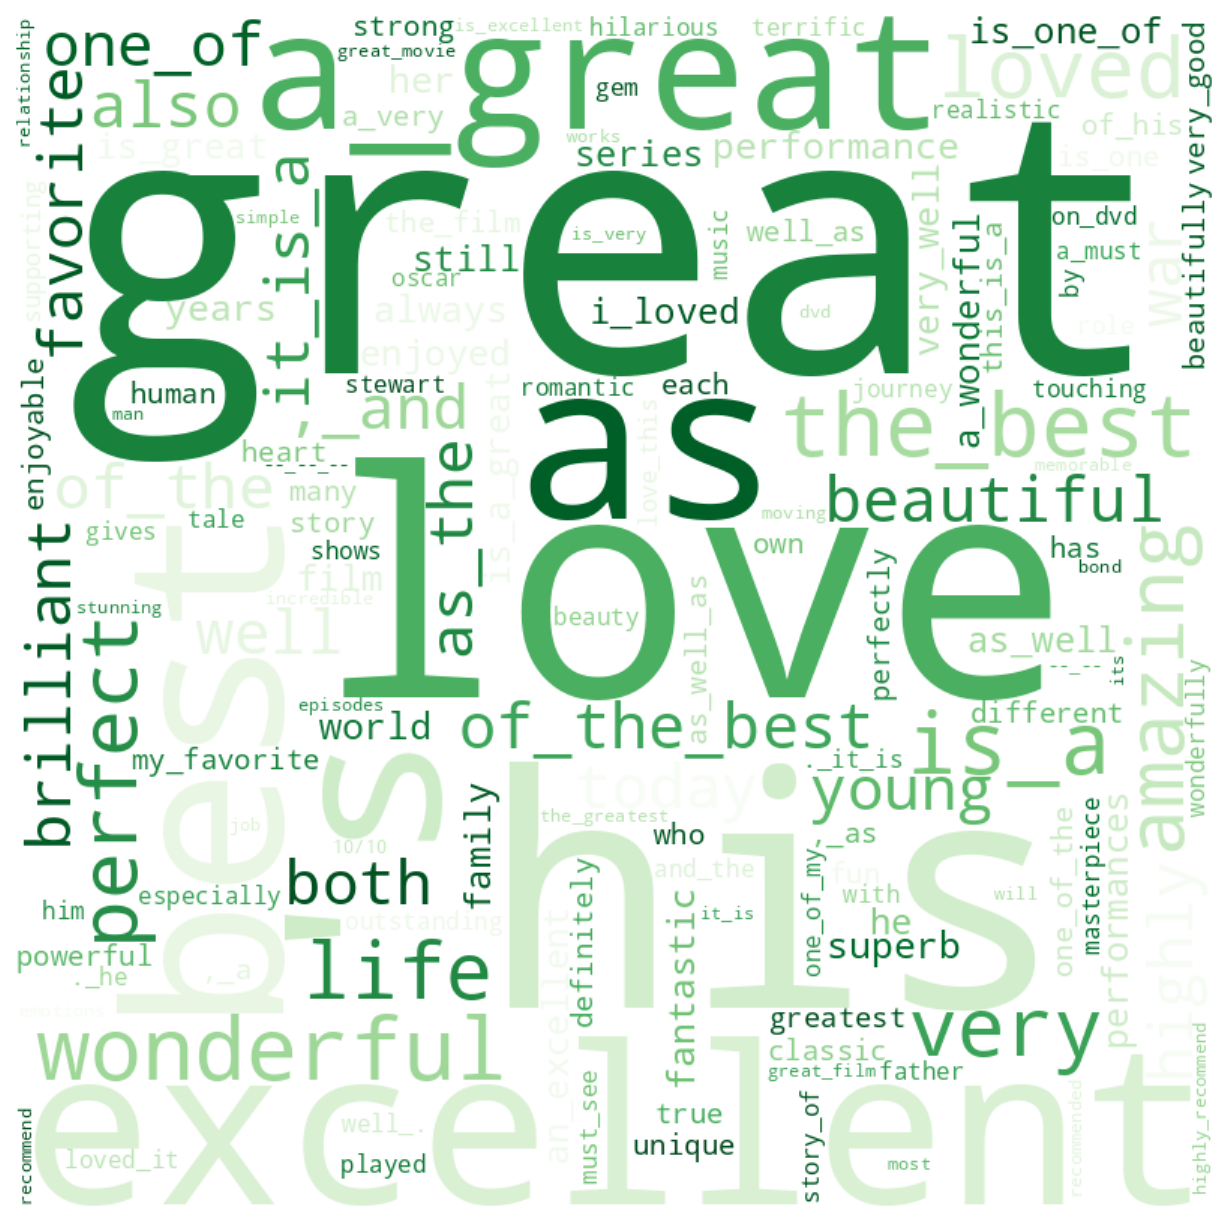
\includegraphics[width=\textwidth]{figures/analysis/tokens_lower_positive_wordcloud.pdf}
		\caption{Extracted positive words (total kept: \num{19172})}
		\label{fig:tokens_lower_positive}
	\end{subfigure}
	\hfill
	\begin{subfigure}[b]{0.30\textwidth}
		\centering
		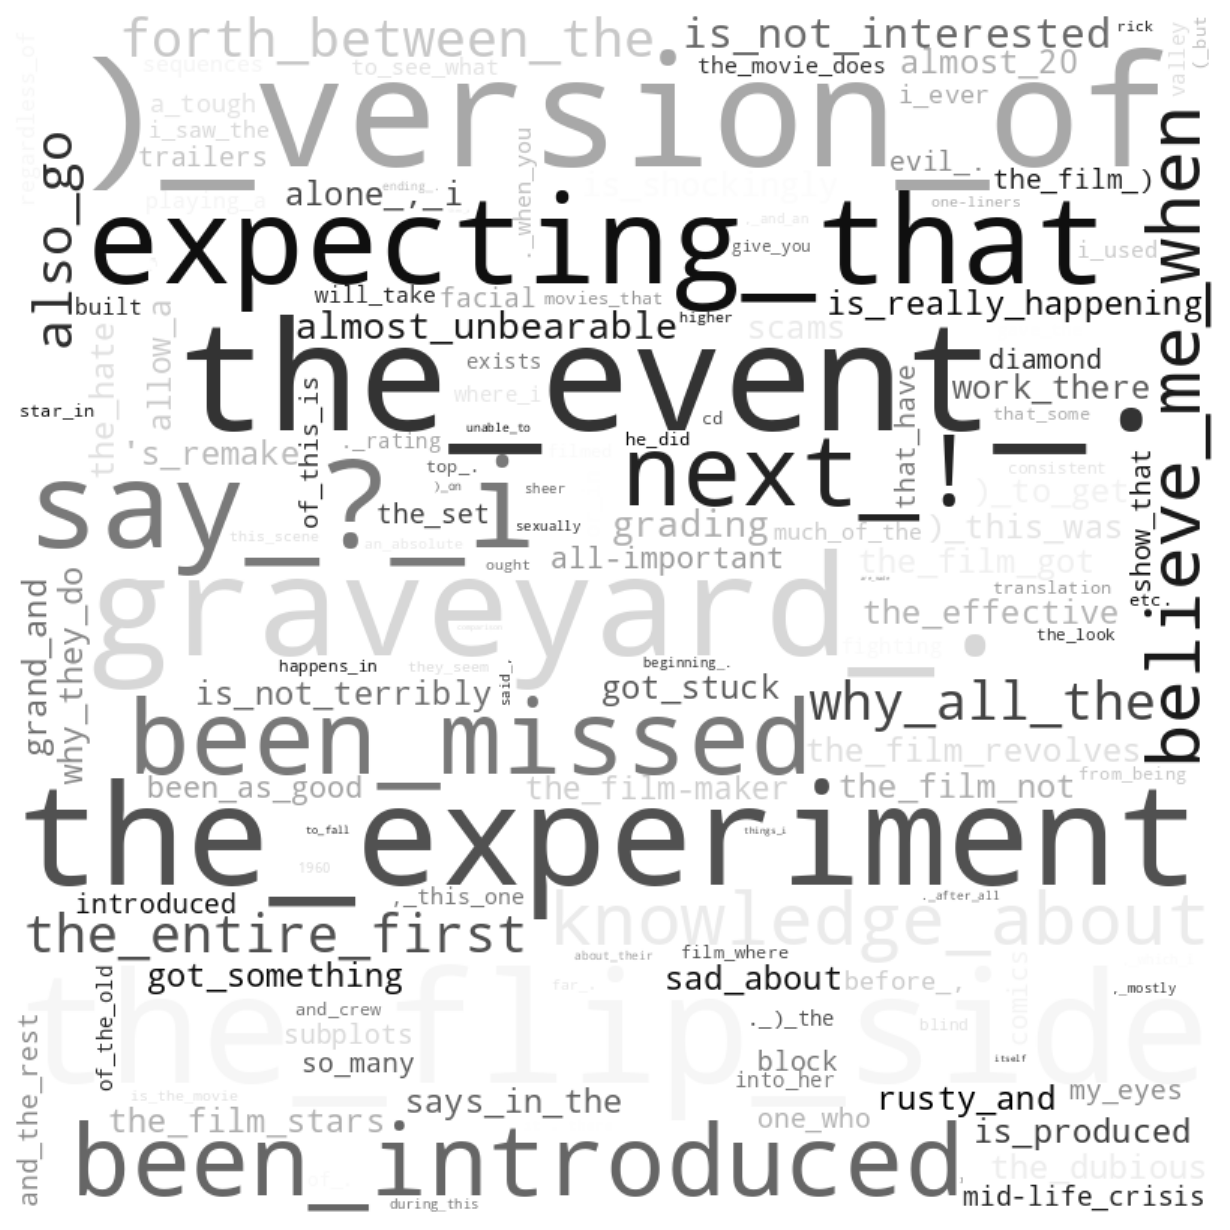
\includegraphics[width=\textwidth]{figures/analysis/tokens_lower_neutral_wordcloud.pdf}
		\caption{Extracted neutral words (total discarded: \num{102665})}
		\label{fig:tokens_lower_neutral}
	\end{subfigure}
	\hfill
	\begin{subfigure}[b]{0.30\textwidth}
		\centering
		
\includegraphics[width=\textwidth]{figures/analysis/tokens_lower_negative_wordcloud.pdf}
		\caption{Extracted negative words (total kept: \num{17178})}
		\label{fig:tokens_lower_negative}
	\end{subfigure}
	\caption{Word clouds for \code{tokens\_lower} (kept and discarded by $\zscore$-score).}
	\label{fig:tokens_lower_clouds}
\end{figure*}

\begin{figure*}[tbp]%[htbp]
	\begin{subfigure}[b]{0.30\textwidth}
		\centering
		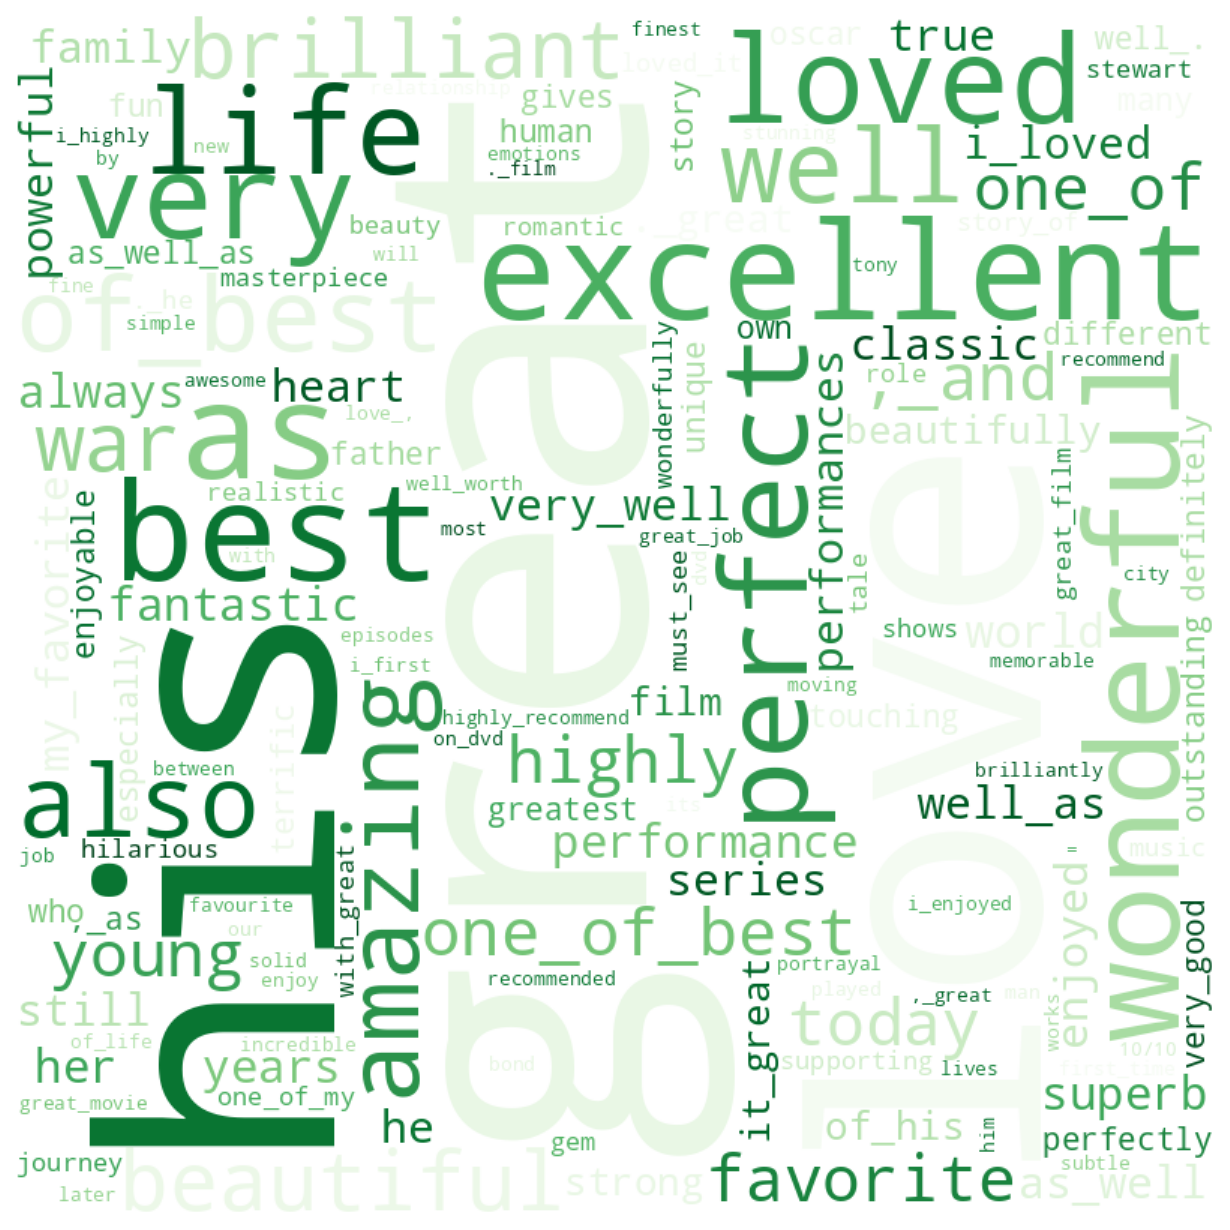
\includegraphics[width=\textwidth]{figures/analysis/tokens_filtered_positive_wordcloud.pdf}
		\caption{Extracted positive words (total kept: \num{15794})}
		\label{fig:tokens_filtered_positive}
	\end{subfigure}
	\hfill
	\begin{subfigure}[b]{0.30\textwidth}
		\centering
		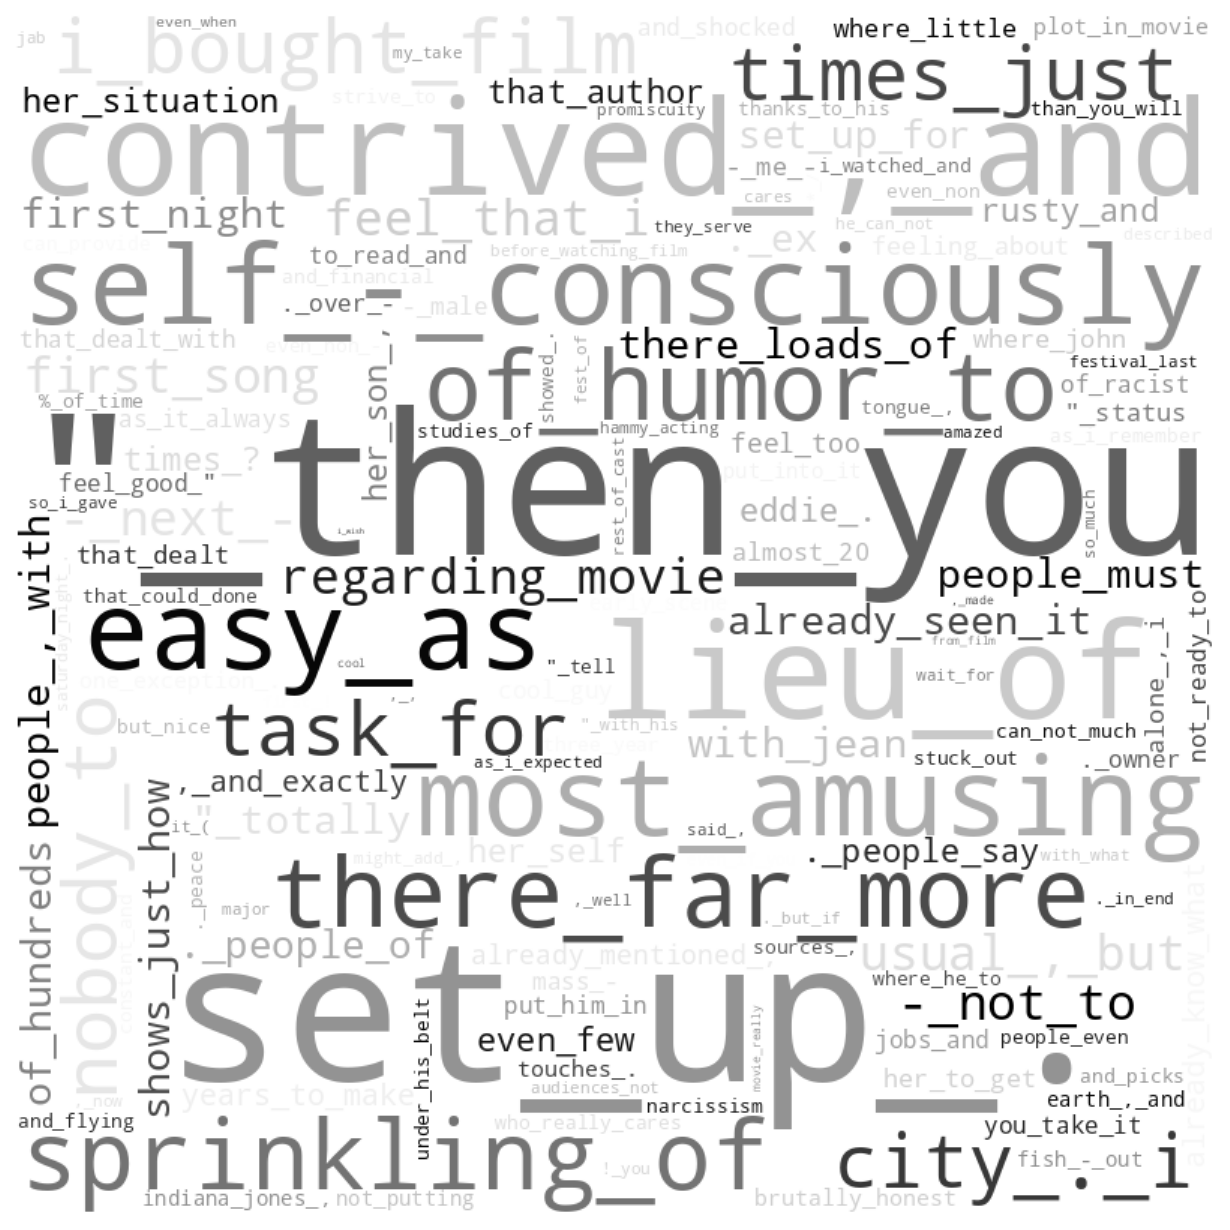
\includegraphics[width=\textwidth]{figures/analysis/tokens_filtered_neutral_wordcloud.pdf}
		\caption{Extracted neutral words (total discarded: \num{85174})}
		\label{fig:tokens_filtered_neutral}
	\end{subfigure}
	\hfill
	\begin{subfigure}[b]{0.30\textwidth}
		\centering
		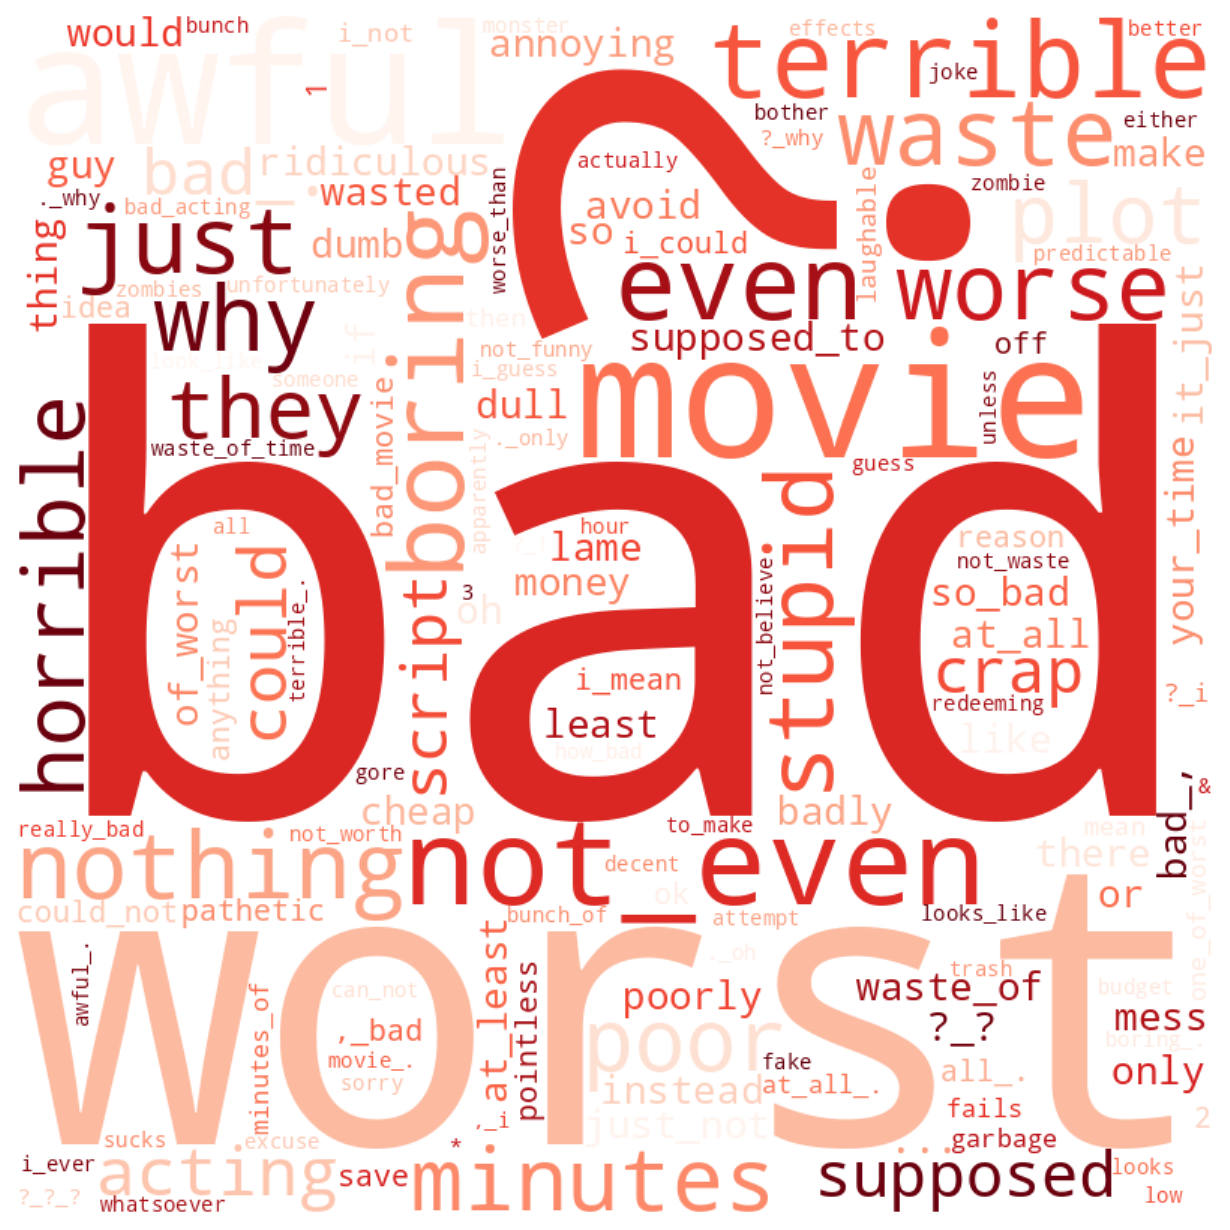
\includegraphics[width=\textwidth]{figures/analysis/tokens_filtered_negative_wordcloud.pdf}
		\caption{Extracted negative words (total kept: \num{14268})}
		\label{fig:tokens_filtered_negative}
	\end{subfigure}
	\caption{Word clouds for \code{tokens\_filtered} (kept and discarded by $\zscore$-score).}
	\label{fig:tokens_filtered_clouds}
\end{figure*}

%\paragraph{Observations}
It is worth noting that the results are easily interpretable. Tokens such as \literal{great} or \literal{love} indicate positive sentiment, while \literal{bad}, \literal{worst}, or \literal{boring} indicate negative feelings towards a movie. It is also interesting that \literal{his}, \literal{episodes}, or \literal{music} appear in the positive group, suggesting that people tend to be more descriptive when they write a positive review. Tokens such as \literal{?}, \literal{why}, and \literal{...} appear in the negative reviews.

\subsubsection{Impact of Custom Vectorization} \label{sec:Impact-of-Custom-Vectorization}

Instead of relying on the default \code{CountVectorizer}, the standard regular expression tokenization is bypassed. After the vectorization, neutral tokens are pruned based on their calculated $\zscore$-scores resulting in Custom BoW (\custombow) and Custom TF-IDF (\customtfidf).

The following test evaluates various tokenization representations to identify the optimal $\zscore$-score pruning threshold, utilizing the best-performing model from the previous stage as a baseline. As illustrated in Figure~\ref{fig:zscore_threshold}, the models' macro $F_1$-scores can remain highly stable even when pruning is applied. However, the effectiveness of pruning is dependent on the chosen feature representation. For the linear SVM utilizing a \custombow{}, statistical pruning proves not applicable; performance degrades immediately, making $\zscore=0$ (no pruning) the optimal threshold. For the \logreg{} model with \custombow{}, the performance remains stable up to a threshold of $\zscore=1$ before declining.

A particularly interesting pattern emerges when utilizing the \customtfidf{} representation. For both the linear SVM and \logreg{} models, the optimal pruning threshold shifts significantly to $\zscore=2$. At this threshold, the SVM maintains its peak baseline performance despite a substantial reduction in the feature space. Notably, the \logreg{} model exhibits a slight increase in its $F_1$-score, suggesting that the targeted removal of neutral features actively improves the model's ability to generalize.

\begin{figure*}[htbp]%[htbp]
	\centering
	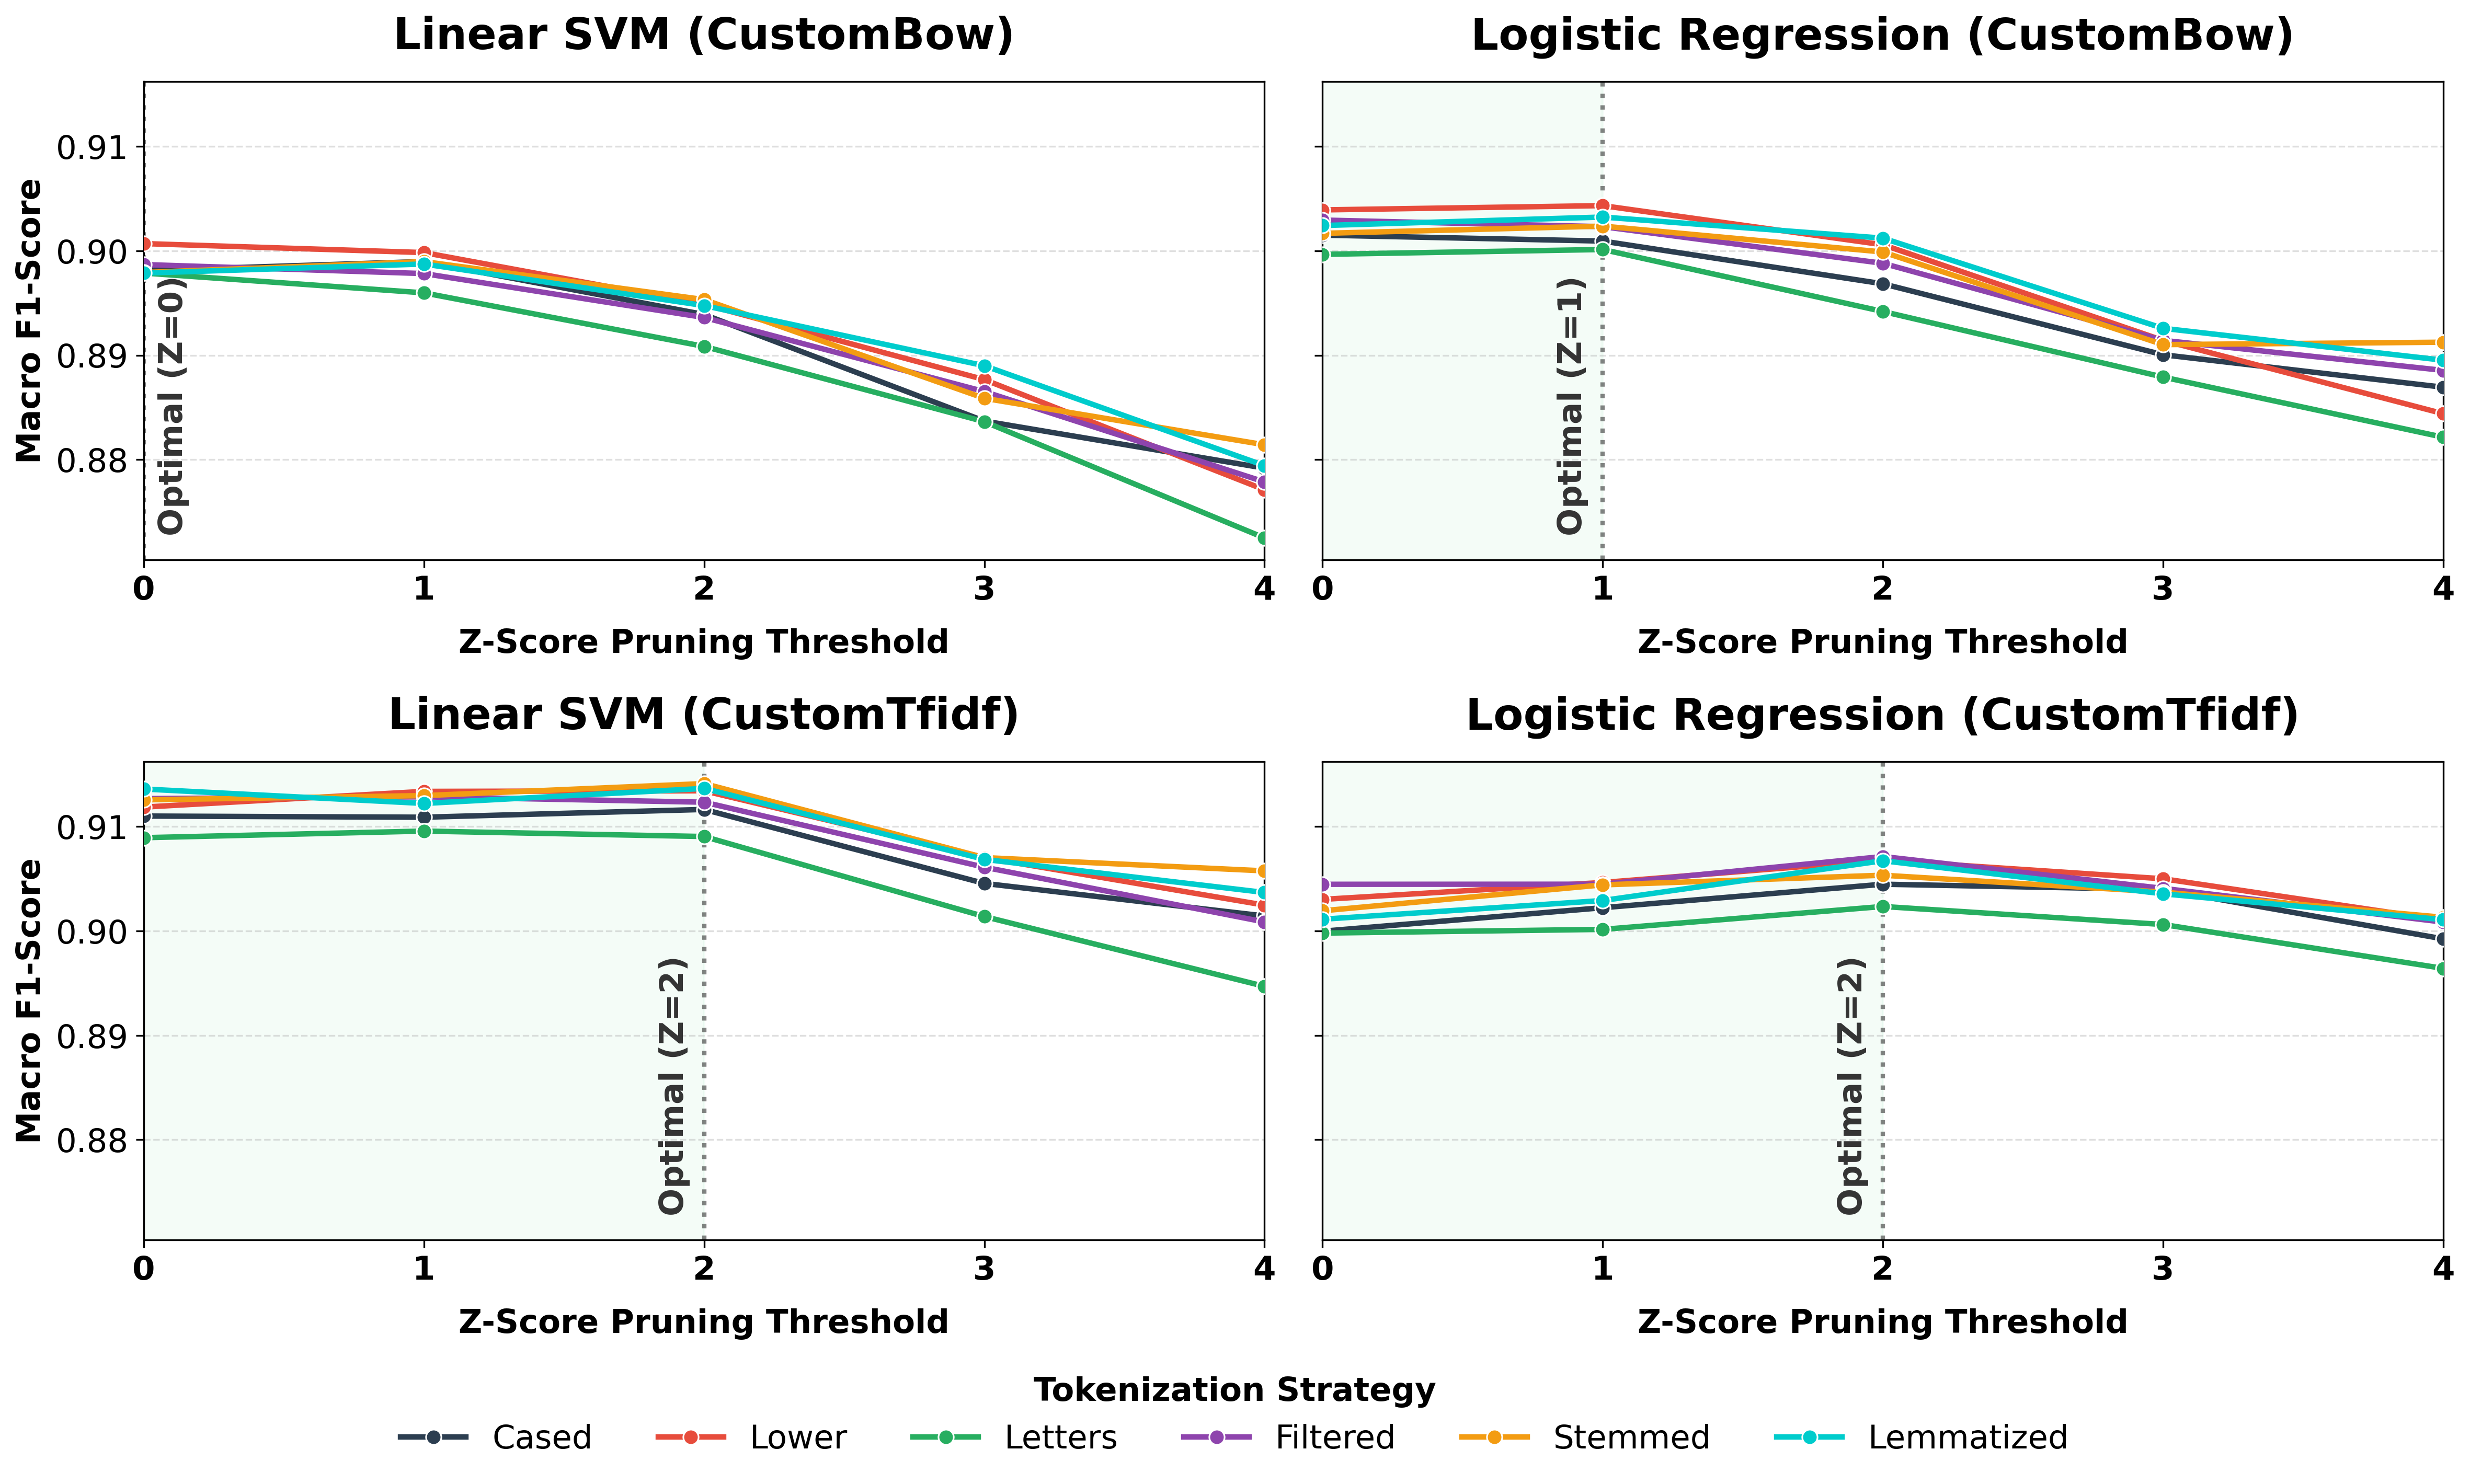
\includegraphics[width=1\textwidth]{./figures/analysis/zscore_threshold.png}
	\caption{Impact of neutral vocabulary pruning on macro $F_1$-score. The $2 \times 2$ grid compares CustomBow (top row) and CustomTfidf (bottom row) representations across SVM (left column) and \logreg{} (right column) models. Line colors distinguish the six tokenization strategies. Vertical dotted lines annotate the optimal pruning threshold, with the shaded green regions highlighting the acceptable threshold range prior to performance loss.}
	\label{fig:zscore_threshold}
\end{figure*}

\paragraph{Impact of Token Type}

As detailed in Table~\ref{tab:McNemarE2}, the most effective token representations rely on stemming, lemmatization, and simple lowercasing. The optimal configuration utilizes stemmed tokens paired with a $\zscore$-score pruning threshold of $\zscore=2$, achieving a peak accuracy of $91.41\%$ ($\mcnemarp = 0.0125$). Lemmatization/Stemming collapses tokens to their morphological roots and thus reduces the feature dimensionality compared to standard tokenization. Additionally, the lemmatized representations at pruning thresholds $\zscore=0$ and $\zscore=2$ achieve a nearly identical accuracy---reducing the dimensionality even more---this shows that pruning can be employed without negatively affecting the accuracy.

\begin{table*} [tbp]%[htbp]
	\centering
	\caption{McNemar test results comparing the baseline TF-IDF representation against custom (\customtfidf{}) representations with different $\zscore$-score pruning values. Only SVM models are considered. Bold text indicates a statistically significant difference ($\mcnemarp < 0.05$) relative to the baseline, with arrows denoting the direction of the change in accuracy.}	\label{tab:McNemarE2}
	\begin{tabular}{llllrcc}
		\toprule
		& Text & Representation & Model & $\accuracy$ & $\uparrow$/$\downarrow$ & $\mcnemarp$-value \\
		\midrule
		\textbf{0} & \textbf{Tokens Stemmed} & \textbf{\customtfidf{} (\zscore2)} & \textbf{SVM} & \textbf{91.41\%} & \textbf{$\uparrow$} & \textbf{0.012517} \\
		\textbf{1} & \textbf{Tokens Lemmatized} & \textbf{\customtfidf{} (\zscore2)} & \textbf{SVM} & \textbf{91.37\%} & \textbf{$\uparrow$} & \textbf{0.020340} \\
		\textbf{2} & \textbf{Tokens Lemmatized} & \textbf{\customtfidf{} (\zscore0)} & \textbf{SVM} & \textbf{91.36\%} & \textbf{$\uparrow$} & \textbf{0.010486} \\
		\textbf{3} & \textbf{Tokens Lower} & \textbf{\customtfidf{} (\zscore2)} & \textbf{SVM} & \textbf{91.34\%} & \textbf{$\uparrow$} & \textbf{0.026857} \\
		\textbf{4} & \textbf{Tokens Lower} & \textbf{\customtfidf{} (\zscore1)} & \textbf{SVM} & \textbf{91.34\%} & \textbf{$\uparrow$} & \textbf{0.018008} \\
		\textbf{5} & \textbf{Tokens Stemmed} & \textbf{\customtfidf{} (\zscore1)} & \textbf{SVM} & \textbf{91.30\%} & \textbf{$\uparrow$} & \textbf{0.049788} \\
		\textbf{6} & \textbf{Expanded and Lower} & \textbf{TF-IDF} & \textbf{SVM} & \textbf{90.98\%} & \textbf{} & \textbf{Baseline} \\
		\textbf{7} & \textbf{Tokens Stemmed} & \textbf{\customtfidf{} (\zscore4)} & \textbf{SVM} & \textbf{90.58\%} & \textbf{$\downarrow$} & \textbf{0.047471} \\
		\textbf{8} & \textbf{Tokens Cased} & \textbf{\customtfidf{} (\zscore3)} & \textbf{SVM} & \textbf{90.46\%} & \textbf{$\downarrow$} & \textbf{0.006363} \\
		\textbf{9} & \textbf{Tokens Lemmatized} & \textbf{\customtfidf{} (\zscore4)} & \textbf{SVM} & \textbf{90.37\%} & \textbf{$\downarrow$} & \textbf{0.002455} \\
		\textbf{10} & \textbf{Tokens Lower} & \textbf{\customtfidf{} (\zscore4)} & \textbf{SVM} & \textbf{90.25\%} & \textbf{$\downarrow$} & \textbf{0.000225} \\
		\textbf{11} & \textbf{Tokens Cased} & \textbf{\customtfidf{} (\zscore4)} & \textbf{SVM} & \textbf{90.15\%} & \textbf{$\downarrow$} & \textbf{0.000044} \\
		\textbf{12} & \textbf{Tokens Letters} & \textbf{\customtfidf{} (\zscore3)} & \textbf{SVM} & \textbf{90.14\%} & \textbf{$\downarrow$} & \textbf{0.000005} \\
		\textbf{13} & \textbf{Tokens Filtered} & \textbf{\customtfidf{} (\zscore4)} & \textbf{SVM} & \textbf{90.09\%} & \textbf{$\downarrow$} & \textbf{0.000013} \\
		\textbf{14} & \textbf{Tokens Letters} & \textbf{\customtfidf{} (\zscore4)} & \textbf{SVM} & \textbf{89.47\%} & \textbf{$\downarrow$} & \textbf{0.000000} \\
		15 & Tokens Filtered & \customtfidf{} (\zscore1) & SVM & 91.29\% &  & 0.059020 \\
		16 & Tokens Filtered & \customtfidf{} (\zscore0) & SVM & 91.27\% &  & 0.065874 \\
		17 & Tokens Stemmed & \customtfidf{} (\zscore0) & SVM & 91.26\% &  & 0.075040 \\
		18 & Tokens Filtered & \customtfidf{} (\zscore2) & SVM & 91.23\% &  & 0.147101 \\
		19 & Tokens Lemmatized & \customtfidf{} (\zscore1) & SVM & 91.22\% &  & 0.119306 \\
		20 & Tokens Lower & \customtfidf{} (\zscore0) & SVM & 91.19\% &  & 0.141313 \\
		21 & Tokens Cased & \customtfidf{} (\zscore2) & SVM & 91.17\% &  & 0.287989 \\
		22 & Tokens Cased & \customtfidf{} (\zscore0) & SVM & 91.10\% &  & 0.434486 \\
		23 & Tokens Cased & \customtfidf{} (\zscore1) & SVM & 91.09\% &  & 0.500669 \\
		24 & Tokens Letters & \customtfidf{} (\zscore1) & SVM & 90.96\% &  & 0.929637 \\
		25 & Tokens Letters & \customtfidf{} (\zscore2) & SVM & 90.91\% &  & 0.681427 \\
		26 & Tokens Letters & \customtfidf{} (\zscore0) & SVM & 90.89\% &  & 0.490824 \\
		27 & Tokens Stemmed & \customtfidf{} (\zscore3) & SVM & 90.70\% &  & 0.161398 \\
		28 & Tokens Lower & \customtfidf{} (\zscore3) & SVM & 90.70\% &  & 0.147175 \\
		29 & Tokens Lemmatized & \customtfidf{} (\zscore3) & SVM & 90.69\% &  & 0.125708 \\
		30 & Tokens Filtered & \customtfidf{} (\zscore3) & SVM & 90.61\% &  & 0.060745 \\
		\bottomrule
	\end{tabular}
\end{table*}

While a few configurations at $\zscore=1$ and $\zscore=2$ yield improvements over the baseline ($\uparrow$), the vast majority of combinations between $\zscore=0$ and $\zscore=3$ result in $\mcnemarp$-values greater than $0.05$. This indicates that for most representation strategies, moderate statistical pruning perfectly maintains classification performance on par with the unpruned baseline. Significant degradation ($\downarrow$) only begins to manifest under aggressive pruning at $\zscore=4$.

As detailed in Table~\ref{tab:McNemarE2logreg}, the simplest representation (Tokens Letters with $\zscore=0$) is chosen as the baseline. Compared to this baseline, a statistically significant increase in accuracy is observed when utilizing more sophisticated representations. 

\begin{table*}[tbp]%[htbp]
	\centering
	\caption{McNemar test results comparing the simplest representation baseline (alphabetical filtering, \customtfidf{} with no pruning) against custom representations with different $\zscore$-score pruning values. Only \logreg{} models are considered. Bold text indicates a statistically significant difference ($\mcnemarp < 0.05$) relative to the baseline, with arrows denoting the direction of the change in accuracy.}
	\label{tab:McNemarE2logreg}
	\begin{tabular}{rlllrcc}
		\toprule
		& Text & Representation & Model & $\accuracy$ & $\uparrow$/$\downarrow$ & $\mcnemarp$-value \\
		\midrule
		\textbf{0} & \textbf{Tokens Filtered} & \textbf{\customtfidf{} (\zscore2)} & \textbf{\logreg{}} & \textbf{90.72\%} & \textbf{$\uparrow$} & \textbf{0.000007} \\
		\textbf{1} & \textbf{Tokens Lower} & \textbf{\customtfidf{} (\zscore2)} & \textbf{\logreg{}} & \textbf{90.68\%} & \textbf{$\uparrow$} & \textbf{0.000003} \\
		\textbf{2} & \textbf{Tokens Lemmatized} & \textbf{\customtfidf{} (\zscore2)} & \textbf{\logreg{}} & \textbf{90.68\%} & \textbf{$\uparrow$} & \textbf{0.000006} \\
		\textbf{3} & \textbf{Tokens Stemmed} & \textbf{\customtfidf{} (\zscore2)} & \textbf{\logreg{}} & \textbf{90.54\%} & \textbf{$\uparrow$} & \textbf{0.000541} \\
		\textbf{4} & \textbf{Tokens Lower} & \textbf{\customtfidf{} (\zscore3)} & \textbf{\logreg{}} & \textbf{90.50\%} & \textbf{$\uparrow$} & \textbf{0.001052} \\
		\textbf{5} & \textbf{Tokens Lower} & \textbf{\customtfidf{} (\zscore1)} & \textbf{\logreg{}} & \textbf{90.47\%} & \textbf{$\uparrow$} & \textbf{0.000508} \\
		\textbf{6} & \textbf{Tokens Filtered} & \textbf{\customtfidf{} (\zscore1)} & \textbf{\logreg{}} & \textbf{90.45\%} & \textbf{$\uparrow$} & \textbf{0.003916} \\
		\textbf{7} & \textbf{Tokens Cased} & \textbf{\customtfidf{} (\zscore2)} & \textbf{\logreg{}} & \textbf{90.45\%} & \textbf{$\uparrow$} & \textbf{0.002850} \\
		\textbf{8} & \textbf{Tokens Filtered} & \textbf{\customtfidf{} (\zscore0)} & \textbf{\logreg{}} & \textbf{90.45\%} & \textbf{$\uparrow$} & \textbf{0.003823} \\
		\textbf{9} & \textbf{Tokens Stemmed} & \textbf{\customtfidf{} (\zscore1)} & \textbf{\logreg{}} & \textbf{90.45\%} & \textbf{$\uparrow$} & \textbf{0.002138} \\
		\textbf{10} & \textbf{Tokens Filtered} & \textbf{\customtfidf{} (\zscore3)} & \textbf{\logreg{}} & \textbf{90.41\%} & \textbf{$\uparrow$} & \textbf{0.014078} \\
		\textbf{11} & \textbf{Tokens Cased} & \textbf{\customtfidf{} (\zscore3)} & \textbf{\logreg{}} & \textbf{90.40\%} & \textbf{$\uparrow$} & \textbf{0.013048} \\
		\textbf{12} & \textbf{Tokens Stemmed} & \textbf{\customtfidf{} (\zscore3)} & \textbf{\logreg{}} & \textbf{90.38\%} & \textbf{$\uparrow$} & \textbf{0.020793} \\
		\textbf{13} & \textbf{Tokens Lemmatized} & \textbf{\customtfidf{} (\zscore3)} & \textbf{\logreg{}} & \textbf{90.36\%} & \textbf{$\uparrow$} & \textbf{0.020176} \\
		\textbf{14} & \textbf{Tokens Lower} & \textbf{\customtfidf{} (\zscore0)} & \textbf{\logreg{}} & \textbf{90.31\%} & \textbf{$\uparrow$} & \textbf{0.017309} \\
		\textbf{15} & \textbf{Tokens Lemmatized} & \textbf{\customtfidf{} (\zscore1)} & \textbf{\logreg{}} & \textbf{90.30\%} & \textbf{$\uparrow$} & \textbf{0.035011} \\
		\textbf{16} & \textbf{Tokens Letters} & \textbf{\customtfidf{} (\zscore0)} & \textbf{\logreg{}} & \textbf{89.98\%} & \textbf{} & \textbf{Baseline} \\
		\textbf{17} & \textbf{Tokens Letters} & \textbf{\customtfidf{} (\zscore4)} & \textbf{\logreg{}} & \textbf{89.64\%} & \textbf{$\downarrow$} & \textbf{0.035752} \\
		18 & Tokens Letters & \customtfidf{} (\zscore2) & \logreg{} & 90.24\% &  & 0.053513 \\
		19 & Tokens Cased & \customtfidf{} (\zscore1) & \logreg{} & 90.23\% &  & 0.108343 \\
		20 & Tokens Stemmed & \customtfidf{} (\zscore0) & \logreg{} & 90.20\% &  & 0.163340 \\
		21 & Tokens Stemmed & \customtfidf{} (\zscore4) & \logreg{} & 90.13\% &  & 0.410827 \\
		22 & Tokens Lemmatized & \customtfidf{} (\zscore0) & \logreg{} & 90.12\% &  & 0.375011 \\
		23 & Tokens Lemmatized & \customtfidf{} (\zscore4) & \logreg{} & 90.11\% &  & 0.477496 \\
		24 & Tokens Lower & \customtfidf{} (\zscore4) & \logreg{} & 90.11\% &  & 0.492971 \\
		25 & Tokens Filtered & \customtfidf{} (\zscore4) & \logreg{} & 90.09\% &  & 0.588993 \\
		26 & Tokens Letters & \customtfidf{} (\zscore3) & \logreg{} & 90.07\% &  & 0.605078 \\
		27 & Tokens Letters & \customtfidf{} (\zscore1) & \logreg{} & 90.02\% &  & 0.785028 \\
		28 & Tokens Cased & \customtfidf{} (\zscore0) & \logreg{} & 90.00\% &  & 0.937425 \\
		29 & Tokens Cased & \customtfidf{} (\zscore4) & \logreg{} & 89.93\% &  & 0.766185 \\
		\bottomrule
	\end{tabular}
\end{table*}

Notably, the filtered representation combined with $\zscore=2$ pruning achieves the highest overall accuracy for the \logreg{} model ($90.72\%$). This contrasts with the earlier findings for the linear SVM, emphasizing that feature selection strategies are highly model-dependent.

\paragraph{Impact of Representation}

The \customtfidf{} representation achieves higher accuracy than the \texttt{\custombow{}} approach across all tested configurations (see Table~\ref{tab:McNemar}). This outcome verifies that the pattern observed in the initial tests (Tables~\ref{tab:McNemarE1a} through~\ref{tab:McNemarE1d}) holds true: TF-IDF outperforms BoW for the sentiment analysis task. The superiority of TF-IDF is robust and largely independent of the tokenization strategy. Additionally, consistent with the trends previously illustrated in Figure~\ref{fig:zscore_threshold}, aggressive pruning at $\zscore=4$ results in performance degradation.

\begin{table*}[tbp]%[htbp]
	\centering
	\caption{McNemar test results comparing the baseline SVM model (lowered tokens, \customtfidf{}, $\zscore=2$) against Custom Bag-of-Words (\custombow{}) representations. Only SVM models are considered. Bold text indicates a statistically significant difference ($\mcnemarp < 0.05$) relative to the baseline, with arrows denoting the direction of the change in accuracy.}
	\label{tab:McNemar}
	\begin{tabular}{rlllrcc}
		\toprule
		& Text & Representation & Model & $\accuracy$ & $\uparrow$/$\downarrow$ & $\mcnemarp$-value \\
		\midrule
		\textbf{0} & \textbf{Tokens Lower} & \textbf{\customtfidf{} (\zscore2)} & \textbf{SVM} & \textbf{91.34\%} & \textbf{} & \textbf{Baseline} \\
		\textbf{1} & \textbf{Tokens Lower} & \textbf{\custombow{} (\zscore0)} & \textbf{SVM} & \textbf{90.07\%} & \textbf{$\downarrow$} & \textbf{0.000000} \\
		\textbf{2} & \textbf{Tokens Lower} & \textbf{\custombow{} (\zscore1)} & \textbf{SVM} & \textbf{89.98\%} & \textbf{$\downarrow$} & \textbf{0.000000} \\
		\textbf{3} & \textbf{Tokens Cased} & \textbf{\custombow{} (\zscore1)} & \textbf{SVM} & \textbf{89.90\%} & \textbf{$\downarrow$} & \textbf{0.000000} \\
		\textbf{4} & \textbf{Tokens Stemmed} & \textbf{\custombow{} (\zscore1)} & \textbf{SVM} & \textbf{89.90\%} & \textbf{$\downarrow$} & \textbf{0.000000} \\
		\textbf{5} & \textbf{Tokens Lemmatized} & \textbf{\custombow{} (\zscore1)} & \textbf{SVM} & \textbf{89.87\%} & \textbf{$\downarrow$} & \textbf{0.000000} \\
		\textbf{6} & \textbf{Tokens Filtered} & \textbf{\custombow{} (\zscore0)} & \textbf{SVM} & \textbf{89.87\%} & \textbf{$\downarrow$} & \textbf{0.000000} \\
		\textbf{7} & \textbf{Tokens Cased} & \textbf{\custombow{} (\zscore0)} & \textbf{SVM} & \textbf{89.81\%} & \textbf{$\downarrow$} & \textbf{0.000000} \\
		\textbf{8} & \textbf{Tokens Stemmed} & \textbf{\custombow{} (\zscore0)} & \textbf{SVM} & \textbf{89.79\%} & \textbf{$\downarrow$} & \textbf{0.000000} \\
		\textbf{9} & \textbf{Tokens Lemmatized} & \textbf{\custombow{} (\zscore0)} & \textbf{SVM} & \textbf{89.79\%} & \textbf{$\downarrow$} & \textbf{0.000000} \\
		\textbf{10} & \textbf{Tokens Letters} & \textbf{\custombow{} (\zscore0)} & \textbf{SVM} & \textbf{89.79\%} & \textbf{$\downarrow$} & \textbf{0.000000} \\
		\textbf{11} & \textbf{Tokens Filtered} & \textbf{\custombow{} (\zscore1)} & \textbf{SVM} & \textbf{89.78\%} & \textbf{$\downarrow$} & \textbf{0.000000} \\
		\textbf{12} & \textbf{Tokens Letters} & \textbf{\custombow{} (\zscore1)} & \textbf{SVM} & \textbf{89.60\%} & \textbf{$\downarrow$} & \textbf{0.000000} \\
		\textbf{13} & \textbf{Tokens Stemmed} & \textbf{\custombow{} (\zscore2)} & \textbf{SVM} & \textbf{89.53\%} & \textbf{$\downarrow$} & \textbf{0.000000} \\
		\textbf{14} & \textbf{Tokens Lower} & \textbf{\custombow{} (\zscore2)} & \textbf{SVM} & \textbf{89.49\%} & \textbf{$\downarrow$} & \textbf{0.000000} \\
		\textbf{15} & \textbf{Tokens Lemmatized} & \textbf{\custombow{} (\zscore2)} & \textbf{SVM} & \textbf{89.48\%} & \textbf{$\downarrow$} & \textbf{0.000000} \\
		\textbf{16} & \textbf{Tokens Cased} & \textbf{\custombow{} (\zscore2)} & \textbf{SVM} & \textbf{89.39\%} & \textbf{$\downarrow$} & \textbf{0.000000} \\
		\textbf{17} & \textbf{Tokens Filtered} & \textbf{\custombow{} (\zscore2)} & \textbf{SVM} & \textbf{89.36\%} & \textbf{$\downarrow$} & \textbf{0.000000} \\
		\textbf{18} & \textbf{Tokens Letters} & \textbf{\custombow{} (\zscore2)} & \textbf{SVM} & \textbf{89.09\%} & \textbf{$\downarrow$} & \textbf{0.000000} \\
		\textbf{19} & \textbf{Tokens Lemmatized} & \textbf{\custombow{} (\zscore3)} & \textbf{SVM} & \textbf{88.90\%} & \textbf{$\downarrow$} & \textbf{0.000000} \\
		\textbf{20} & \textbf{Tokens Lower} & \textbf{\custombow{} (\zscore3)} & \textbf{SVM} & \textbf{88.77\%} & \textbf{$\downarrow$} & \textbf{0.000000} \\
		\textbf{21} & \textbf{Tokens Filtered} & \textbf{\custombow{} (\zscore3)} & \textbf{SVM} & \textbf{88.65\%} & \textbf{$\downarrow$} & \textbf{0.000000} \\
		\textbf{22} & \textbf{Tokens Stemmed} & \textbf{\custombow{} (\zscore3)} & \textbf{SVM} & \textbf{88.59\%} & \textbf{$\downarrow$} & \textbf{0.000000} \\
		\textbf{23} & \textbf{Tokens Cased} & \textbf{\custombow{} (\zscore3)} & \textbf{SVM} & \textbf{88.37\%} & \textbf{$\downarrow$} & \textbf{0.000000} \\
		\textbf{24} & \textbf{Tokens Letters} & \textbf{\custombow{} (\zscore3)} & \textbf{SVM} & \textbf{88.37\%} & \textbf{$\downarrow$} & \textbf{0.000000} \\
		\textbf{25} & \textbf{Tokens Stemmed} & \textbf{\custombow{} (\zscore4)} & \textbf{SVM} & \textbf{88.15\%} & \textbf{$\downarrow$} & \textbf{0.000000} \\
		\textbf{26} & \textbf{Tokens Lemmatized} & \textbf{\custombow{} (\zscore4)} & \textbf{SVM} & \textbf{87.94\%} & \textbf{$\downarrow$} & \textbf{0.000000} \\
		\textbf{27} & \textbf{Tokens Cased} & \textbf{\custombow{} (\zscore4)} & \textbf{SVM} & \textbf{87.92\%} & \textbf{$\downarrow$} & \textbf{0.000000} \\
		\textbf{28} & \textbf{Tokens Filtered} & \textbf{\custombow{} (\zscore4)} & \textbf{SVM} & \textbf{87.79\%} & \textbf{$\downarrow$} & \textbf{0.000000} \\
		\textbf{29} & \textbf{Tokens Lower} & \textbf{\custombow{} (\zscore4)} & \textbf{SVM} & \textbf{87.71\%} & \textbf{$\downarrow$} & \textbf{0.000000} \\
		\textbf{30} & \textbf{Tokens Letters} & \textbf{\custombow{} (\zscore4)} & \textbf{SVM} & \textbf{87.25\%} & \textbf{$\downarrow$} & \textbf{0.000000} \\
		\bottomrule
	\end{tabular}
\end{table*}

\paragraph{Ablation Study}

In Figure~\ref{fig:ablation_study}, the BoW and TF-IDF labels denote the unpruned token representations. Meanwhile, \custombow{} and \customtfidf{} designate where pruning ($\zscore=2$) has been applied.

For the BoW, various tokenization strategies yield no improvement over the \texttt{Expanded and Lower} baseline for either the linear SVM or \logreg{} models. Furthermore, when statistical pruning is introduced (\custombow{}), performance consistently degrades across all configurations; removing vocabulary features universally harms the predictive power of BoW.

In contrast, the TF-IDF representations exhibit a lot of variance. For the linear SVM, only the lemmatized tokenization approach proves significantly better than the TF-IDF Baseline. However, the introduction of $\zscore=2$ pruning actively enhances the model's capabilities, increasing the macro $F_1$-scores for the lowered and stemmed representations. Combining stemming and \customtfidf{} achieves the highest overall performance ($91.41\%$).

For the \logreg{} model, the classification scores are generally lower than those achieved by the SVM. For the BoW approach, pruning either degrades performance (as seen with cased and letter-only tokens) or has no significant effect. However, the introduction of filtering combined with \customtfidf{} pruning proves effective. While isolated tokenization approaches do not have a clear impact on their own, the pruning strategy elevates almost all TF-IDF-based representations for \logreg{}, with the sole exception of the \texttt{Tokens Letters} configuration. The \texttt{Tokens Filtered} representation with $\zscore=2$ pruning outperforms the baseline by over 0.7 percentage points (rising from $89.98\%$ to $90.71\%$).

\begin{figure*}[tbp]%[htbp]
	\centering
	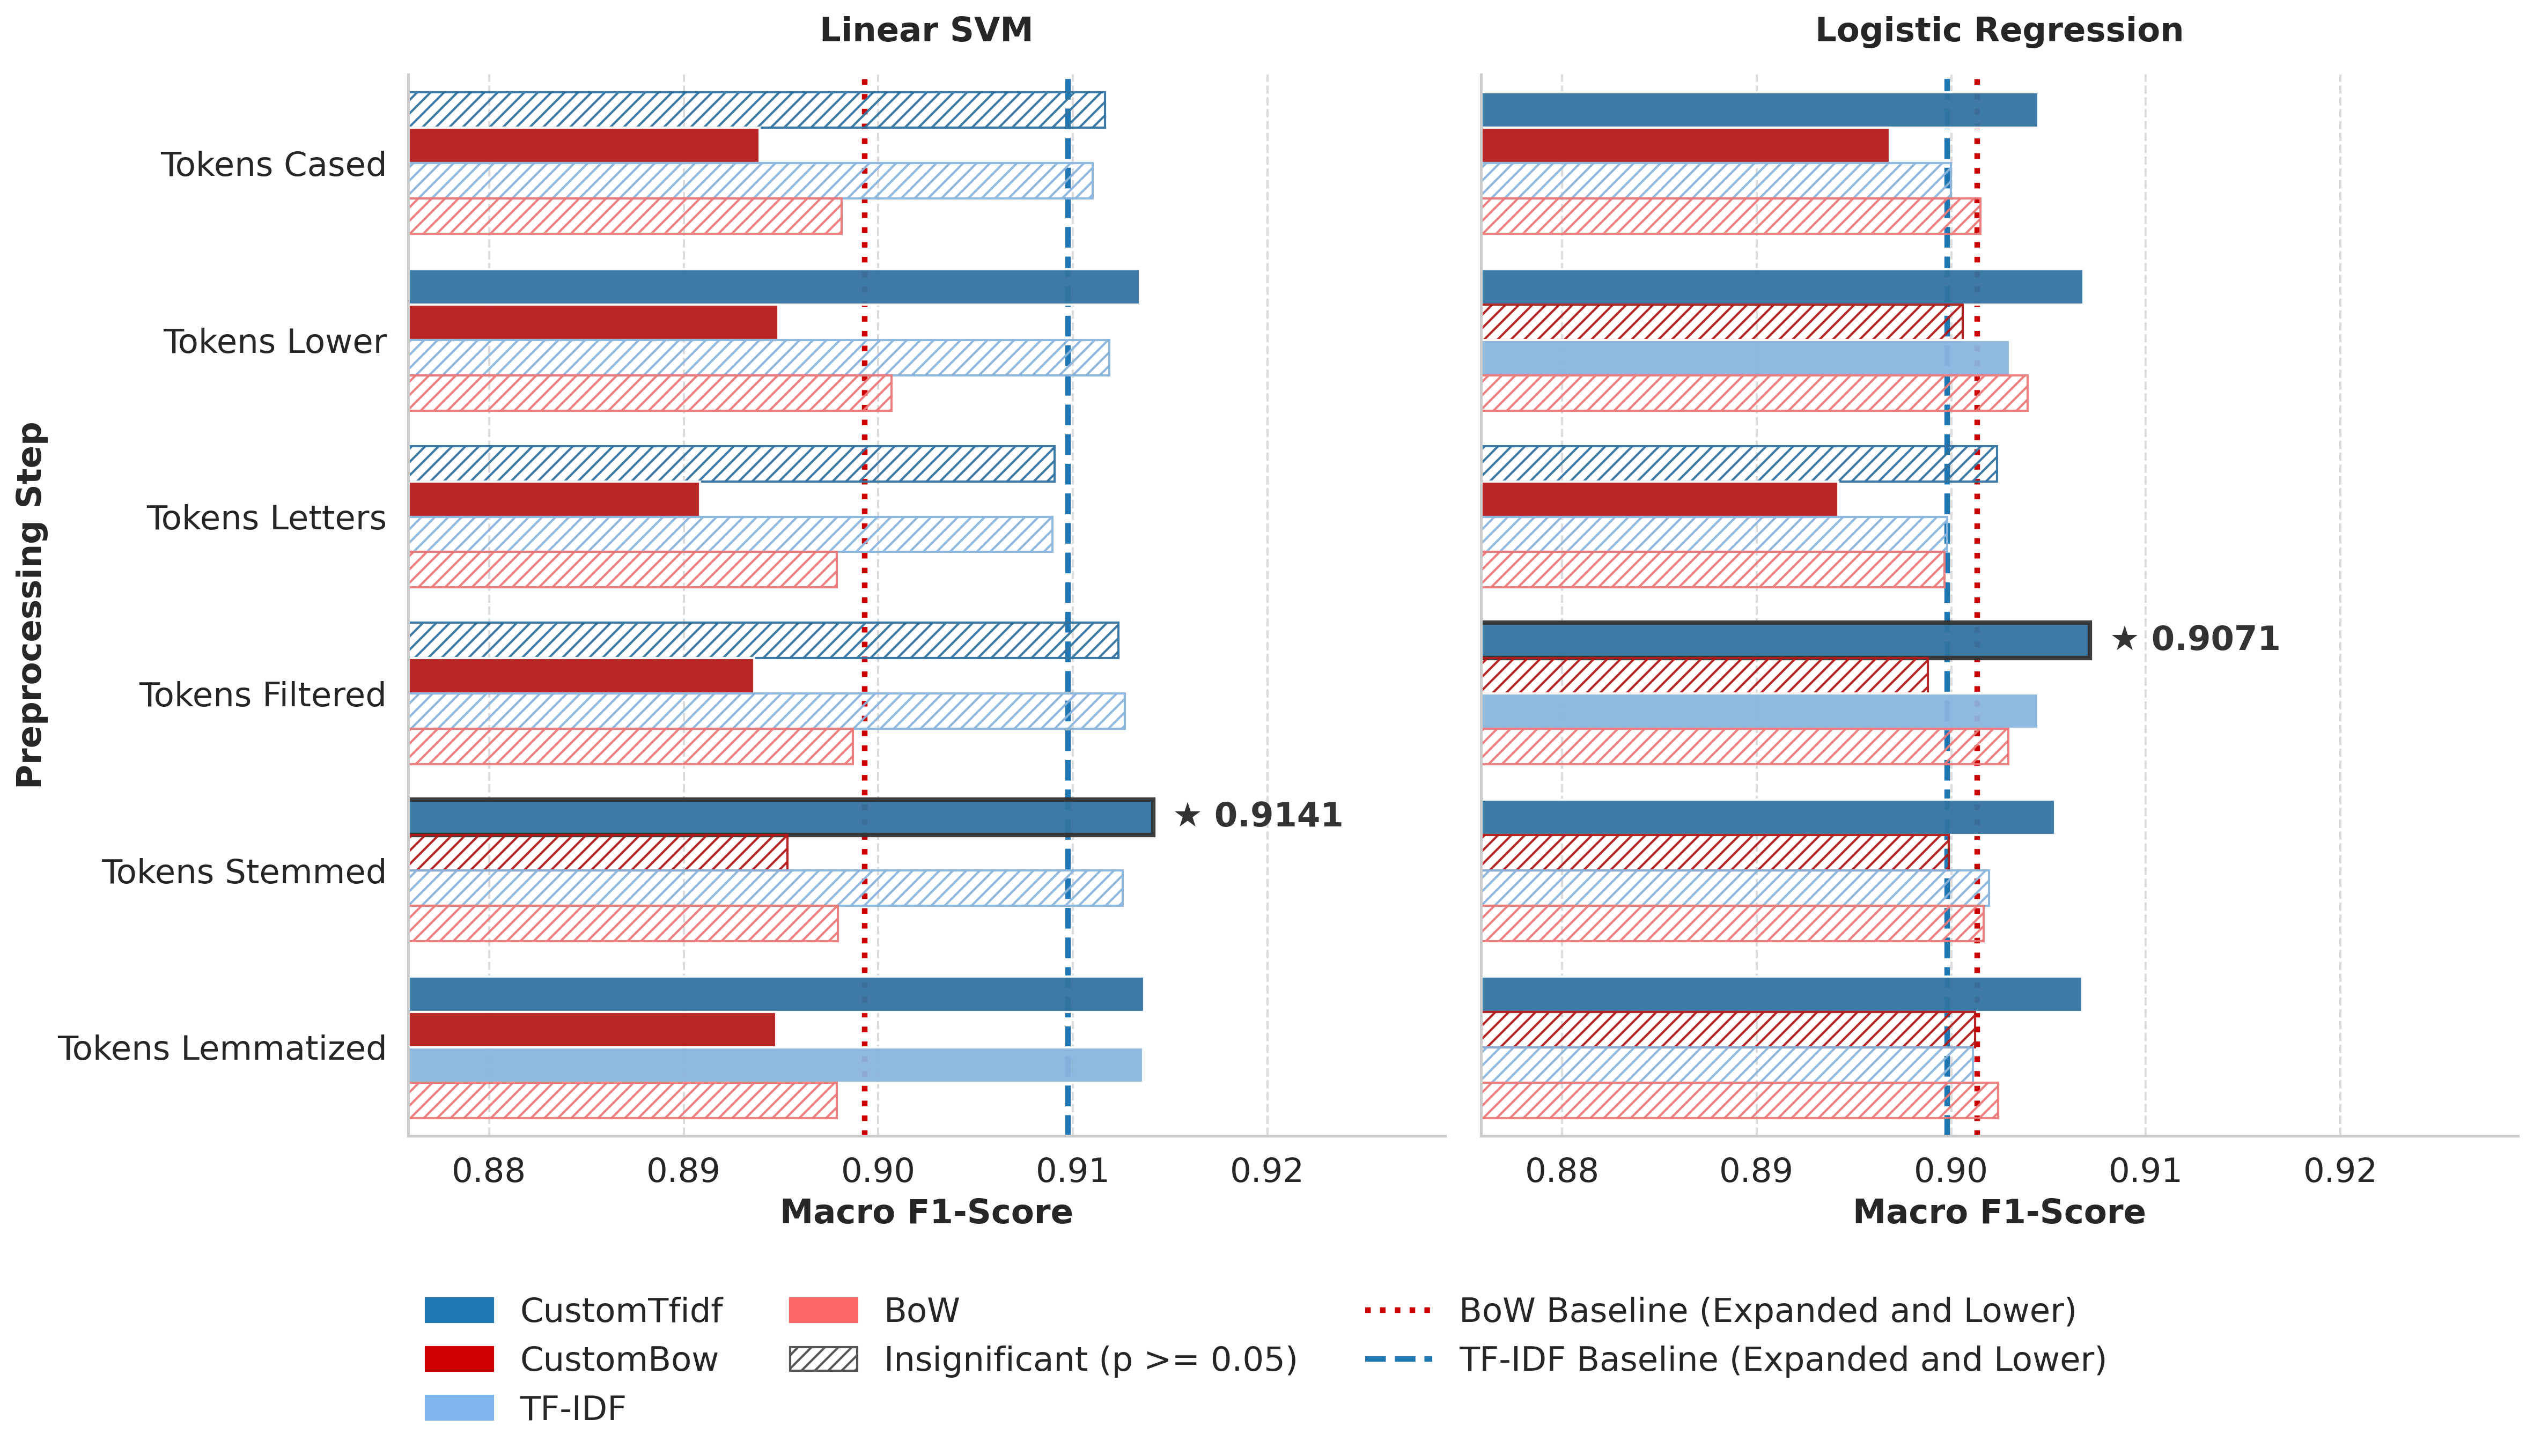
\includegraphics[width=1\textwidth]{./figures/analysis/ablation_study.png}
	\caption{Ablation study evaluating standard tokenized representations versus custom representations with statistical pruning across various preprocessing steps. Bar colors distinguish the representation family (blues for TF-IDF, reds for BoW), vertical lines mark the baseline performance on lower-cased expanded text. Hashed bars indicate results that are not statistically significantly different from their respective baseline ($\mcnemarp \ge 0.05$). The top-performing configurations for each model are outlined and annotated with a star.}
	\label{fig:ablation_study}
\end{figure*}



\subsubsection{Impact of Vocabulary Depth} \label{sec:Impact-of-Vocabulary-Depth}

This test examines the importance of selecting the optimal  $n$-gram range---the vocabulary depth. As depicted in the left panel of Figure~\ref{fig:vocabulary_depth}, expanding the token representation from simple unigrams $(1,1)$ to include bigrams $(1,2)$ yields a substantial increase in the macro $F_1$-score for both the linear SVM and \logreg{} models. However, extending the depth further to include trigrams $(1,3)$ provides only marginal performance gains, illustrating a clear pattern of diminishing returns.

\paragraph{Dimensionality Problem}
While deeper $n$-gram ranges capture richer sequential context, they introduce a severe structural challenge: the explosion of the feature space. The right panel of Figure~\ref{fig:vocabulary_depth} demonstrates that the base vocabulary grows aggressively, swelling from $18{,}471$ unigrams to \num{139015} total features when trigrams are included. Extrapolating this trajectory suggests that exploring even deeper ranges, such as $4$-grams $(1,4)$, would predictably push the raw feature count well beyond \num{190000}. Operating on such massive, highly sparse matrices becomes extremely memory-intensive.

\paragraph{Dimensionality Reduction}
The implementation of statistical pruning ($\zscore=2.0$) effectively mitigates this dimensionality explosion. For the $(1,3)$ vocabulary range, pruning discards over \num{100000} non-discriminative features, compressing the space from \num{139015} down to manageable $36{,}350$ features. This ensures that the classifiers can leverage the contextual richness of higher-order $n$-grams without suffering the standard computational penalties associated with high dimensionality.

\begin{figure*}[tbp]%[htbp]
	\centering
	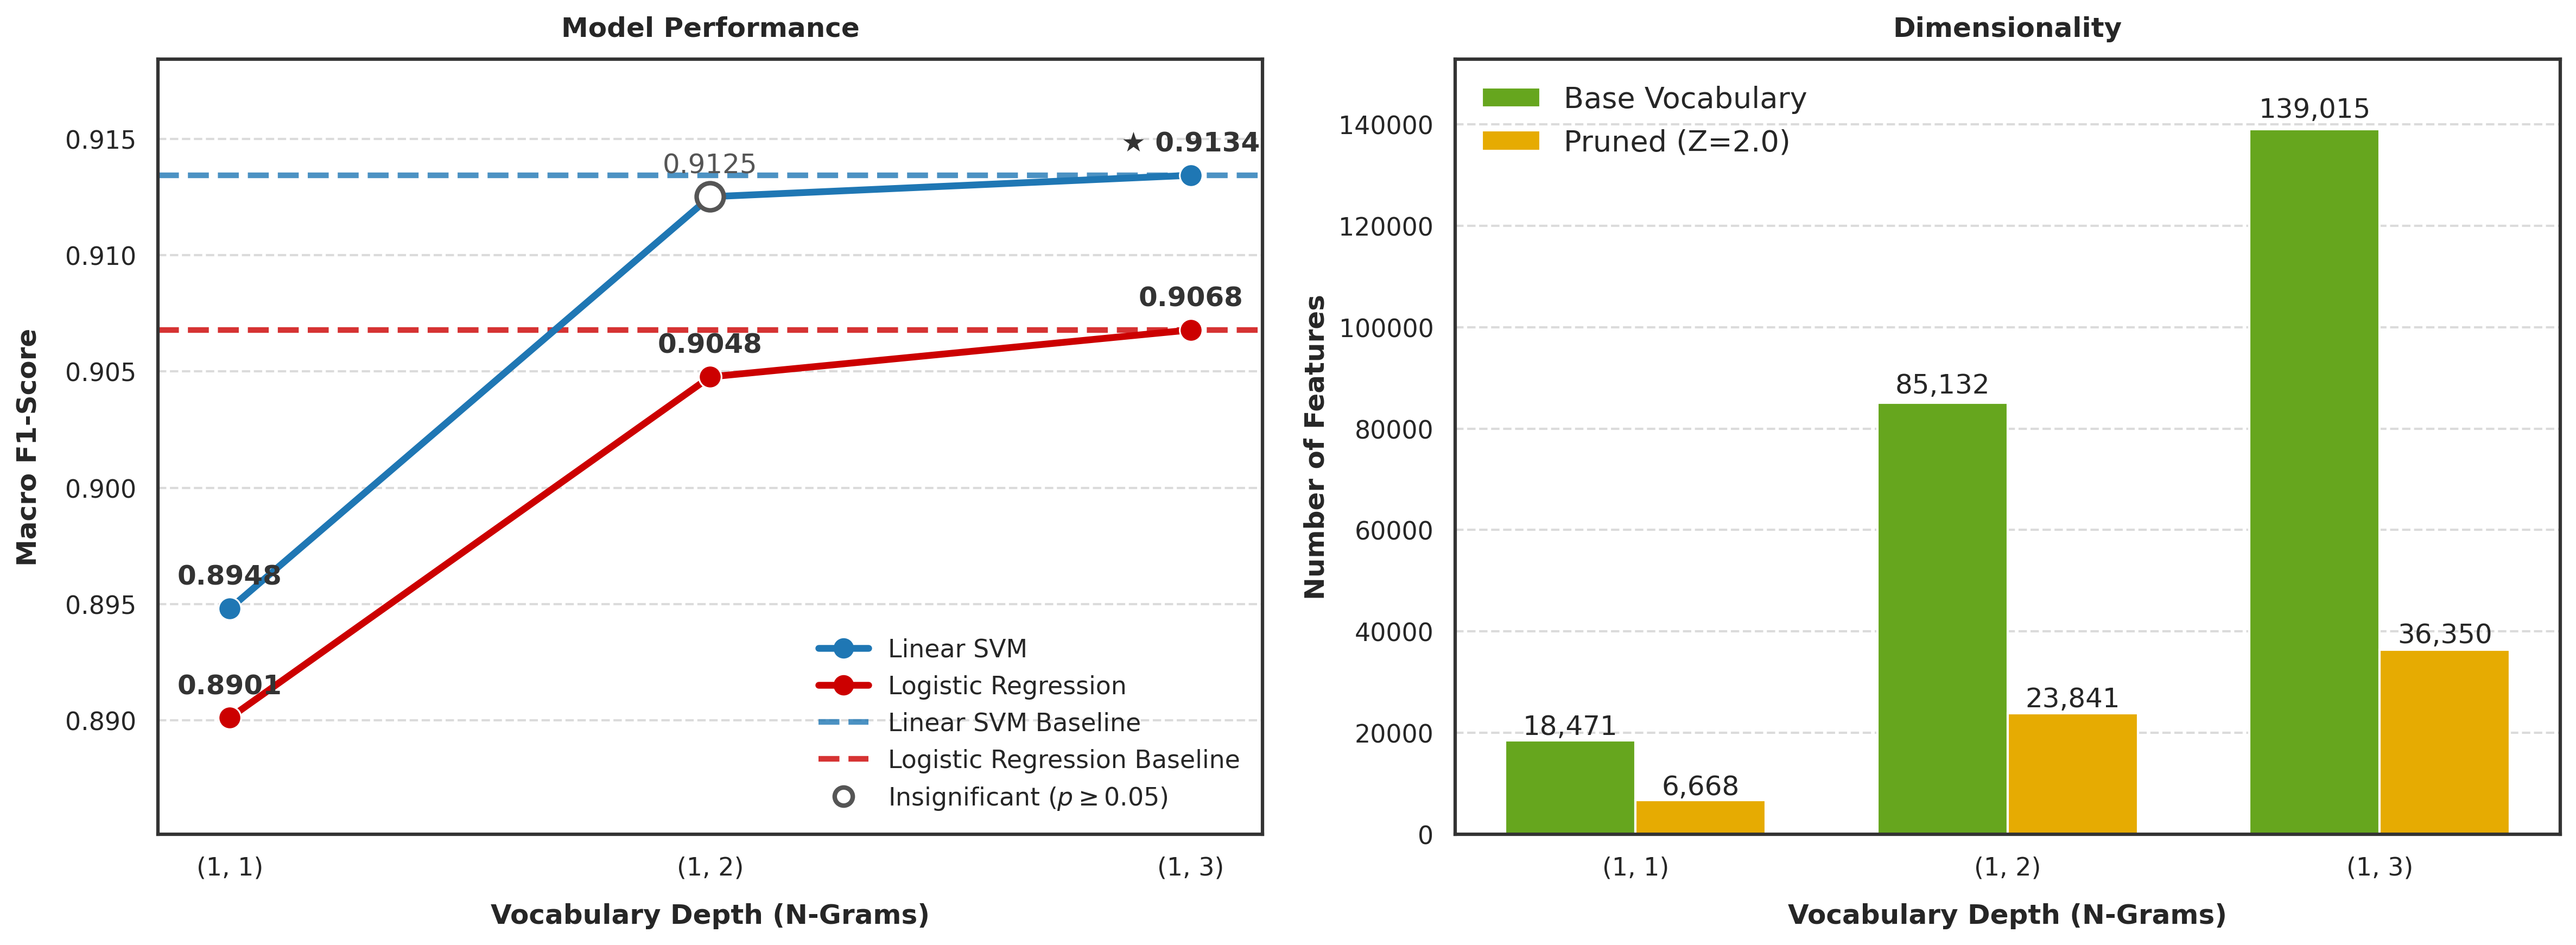
\includegraphics[width=1\textwidth]{./figures/analysis/ngram_experiment_double.png}
	\caption{Performance and dimensionality trends across varying $n$-gram ranges. The left panel illustrates model performance (macro $F_1$-score), where dashed lines indicate the respective baselines for Linear SVM (blue) and \logreg{} (red). Hollow markers denote results that are not statistically significantly different from their baseline ($\mcnemarp \ge 0.05$), and a star highlights the overall best-performing configuration. The right panel highlights the feature space reduction, comparing the base vocabulary size (green bars) against the pruned vocabulary using $\zscore=2.0$ (orange bars).}
	\label{fig:vocabulary_depth}
\end{figure*}

\subsubsection{Impact of Kernel} \label{sec:Impact-of-Kernel}

To assess the influence of the kernel function, a linear SVM is compared against an RBF SVM, using the best previously determined text representation and preprocessing settings (see Table~\ref{tab:McNemarSvms}). Both models were trained on the full training set, with probability calibration performed internally via $5$-fold cross‑validation (\texttt{CalibratedClassifierCV})---no cross-validation accuracy metrics are exported by the calibration procedure. 

Both variants use a fixed \code{max\_iter} limit. The linear SVM with \code{max\_iter=10000} trains and converges in only $1.89$ seconds, achieving $91.34\%$ accuracy. In contrast, the RBF kernel with the same iteration limit trains for \num{2042.05} seconds (over $34$ minutes) and reaches $91.15\%$ accuracy. However, the RBF solver did not converge: it exhausted the maximum number of iterations before reaching the stopping criterion. This indicates that the RBF kernel's optimization landscape is harder to navigate, and requires more time for proper convergence.

When \code{max\_iter} is reduced to \num{1000}, the RBF training time drops to \num{267.07} seconds (approximately $4.5$ minutes), but accuracy falls to $89.03\%$.
The difference between this RBF variant and the linear baseline is significant according to McNemar's test ($\mcnemarp < 0.000001$), whereas the non-converged RBF with \num{10000} iterations does not exhibit a statistically significant difference from the linear SVM ($\mcnemarp = 0.142$).
Overall, the linear kernel yields the highest accuracy and has significantly lower computational cost, making it preferable for the further tests.

\begin{table*}[tbp]
	\centering
	\caption{McNemar's test comparing linear and RBF kernel SVMs, including training times measured on \code{AMD Ryzen 7 5800H with Radeon Graphics} at different iteration limits (\code{max\_iter}).}
	\label{tab:McNemarSvms}
	\begin{tabular}{llllrcc}
		\toprule
		& \code{max\_iter} & Training Time & Model & $\accuracy$ & $\uparrow$/$\downarrow$ & $\mcnemarp$-value \\
		\midrule
		\textbf{0} & \textbf{10,000} & \textbf{1.89 s} & \textbf{Linear SVM} & \textbf{91.34\%} & \textbf{} & \textbf{Baseline} \\
		\textbf{1} & \textbf{1,000} & \textbf{267.07 s} & \textbf{RBF SVM} & \textbf{89.03\%} & \textbf{$\downarrow$} & \textbf{0.000000} \\
		2 & 10,000 & 2042.05 s & RBF SVM & 91.15\% &  & 0.142368 \\
		\bottomrule
	\end{tabular}
\end{table*}

\subsubsection{Impact of Semantic Clustering} \label{sec:Impact-of-Semantic-Clustering}

Semantic clustering groups related $n$-grams to capture conceptual representations. As shown in Figure~\ref{fig:concepts_pos_10000_0}, the cluster containing \literal{great}, \literal{wonderful}, and \literal{amazing} forms the most discriminative positive concept, achieving a $\zscore$-score of \num{44.20}. Clusters focused on structural phrases, such as \literal{his} or \literal{is an} rank among the top positive concepts, reinforcing the earlier observation that reviewers tend to use more descriptive language when expressing a positive opinion.

\begin{figure*}[tbp]%[htbp]
	\centering
	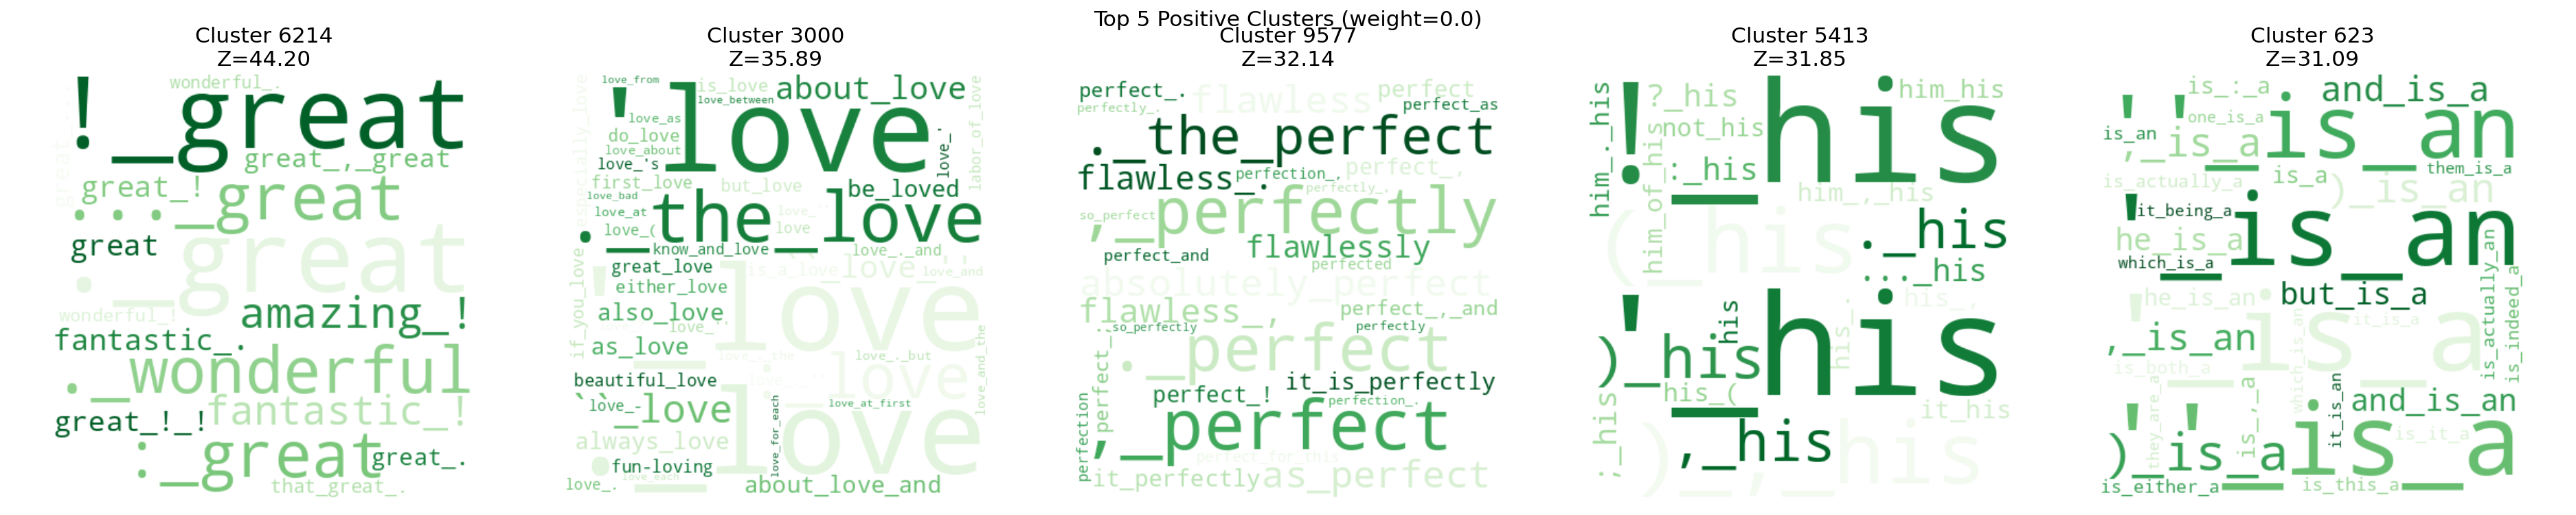
\includegraphics[width=1\textwidth]{./figures/concepts/pos_wc_tokens_lower_k10000_w0.png}
	\caption{Top 5 positive concepts extracted via baseline semantic clustering ($\conceptWeight=0$).}
	\label{fig:concepts_pos_10000_0}
\end{figure*}

Figure~\ref{fig:concepts_neg_10000_0} illustrates that negative clusters contain repeated punctuation. A significant advantage of clustering $n$-grams is that varying permutations of punctuation (e.g., \literal{?!} and \literal{!??}) are grouped into a single conceptual feature, which theoretically could improve the model's ability to generalize noisy text. Other top negative concepts contain direct negative descriptors (e.g., \literal{worst}, \literal{horrible}, \literal{awful}). The cluster containing the phrase \literal{bad, but} appears highly ranked for negativity, even though such phrasing depicts a mitigating clause or mixed sentiment in natural language rather than pure negativity.

\begin{figure*}[tbp]%[htbp]
	\centering
	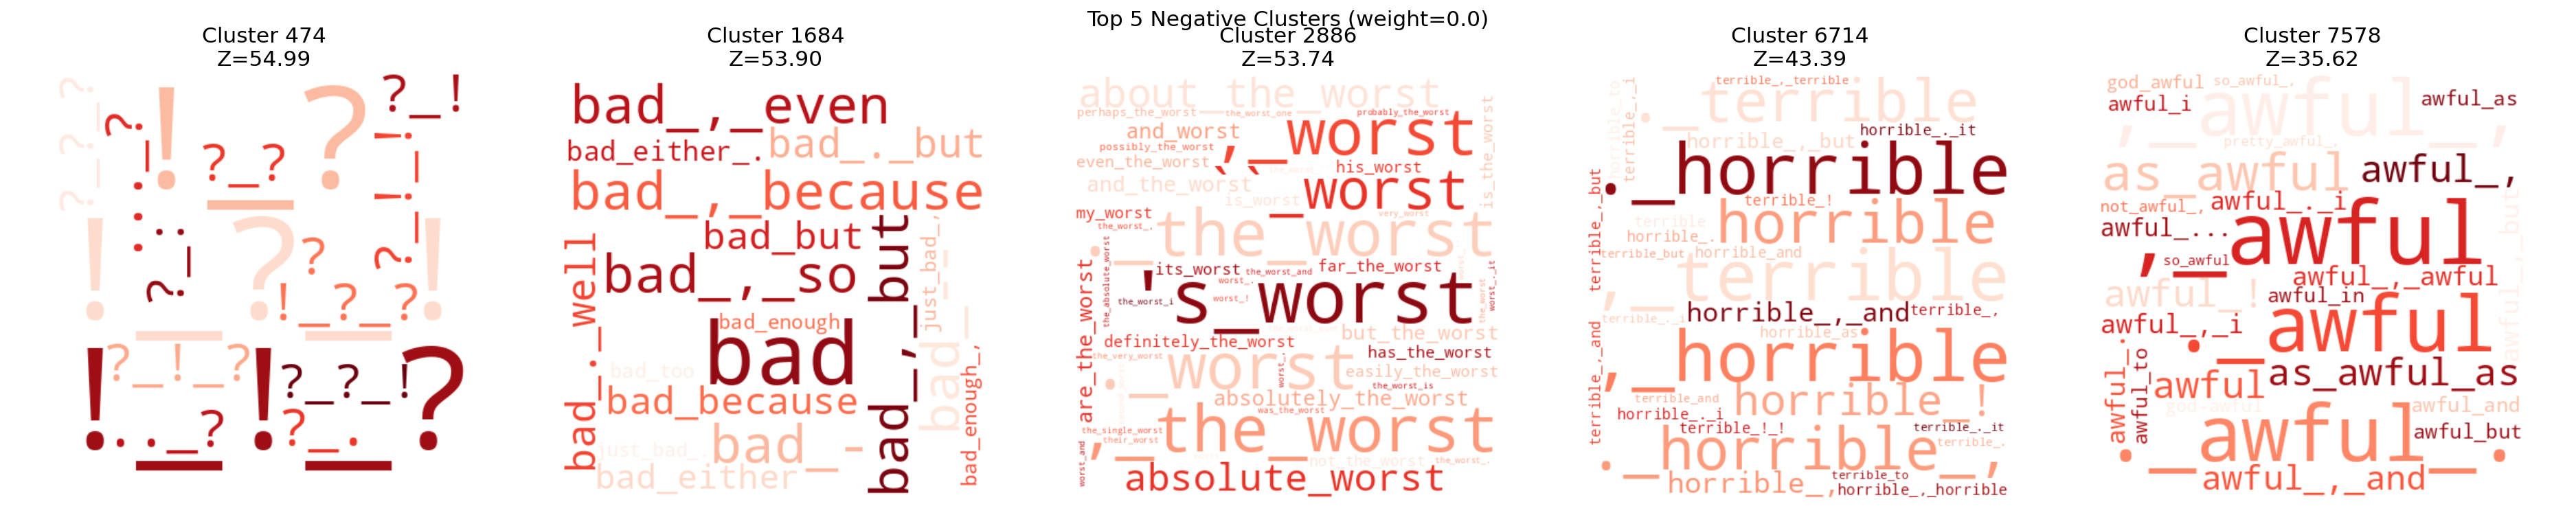
\includegraphics[width=1\textwidth]{./figures/concepts/neg_wc_tokens_lower_k10000_w0.png}
	\caption{Top 5 negative concepts extracted via baseline semantic clustering ($\conceptWeight=0$).}
	\label{fig:concepts_neg_10000_0}
\end{figure*}

\paragraph{Weighted Approach}
Figures~\ref{fig:concepts_pos_10000_10} and \ref{fig:concepts_neg_10000_10} depict that incorporating lexicon-based polarity increases the $\zscore$-score values, and thus produces more cohesive and discriminative clusters. For example, the primary positive cluster expands to integrate \literal{excellent} alongside \literal{great}. Similarly, the \literal{bad} cluster becomes more distinct and captures negative connotations, confirming the effectiveness of the weighting strategy. Descriptive but sentiment-neutral concepts (such as the \literal{his} cluster) decrease in prominence, demonstrating that VADER-weighting effectively prioritizes sentiment signals.

\begin{figure*}[tbp]%[htbp]
	\centering
	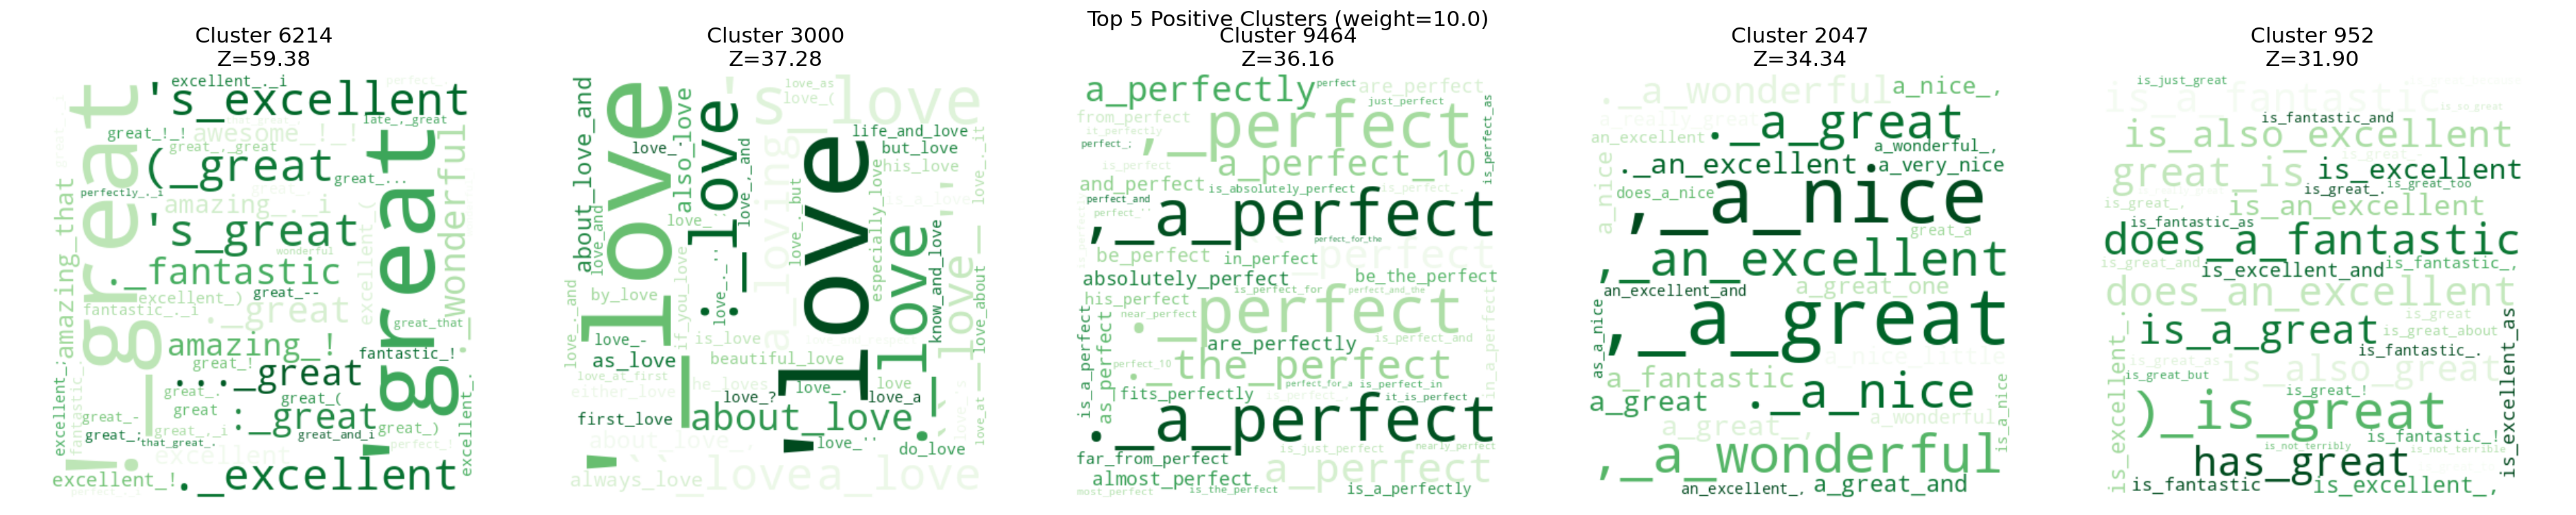
\includegraphics[width=1\textwidth]{./figures/concepts/pos_wc_tokens_lower_k10000_w10.png}
	\caption{Top 5 positive concepts extracted via weighted semantic clustering ($\conceptWeight=10$).}
	\label{fig:concepts_pos_10000_10}
\end{figure*}

\begin{figure*}[tbp]%[htbp]
	\centering
	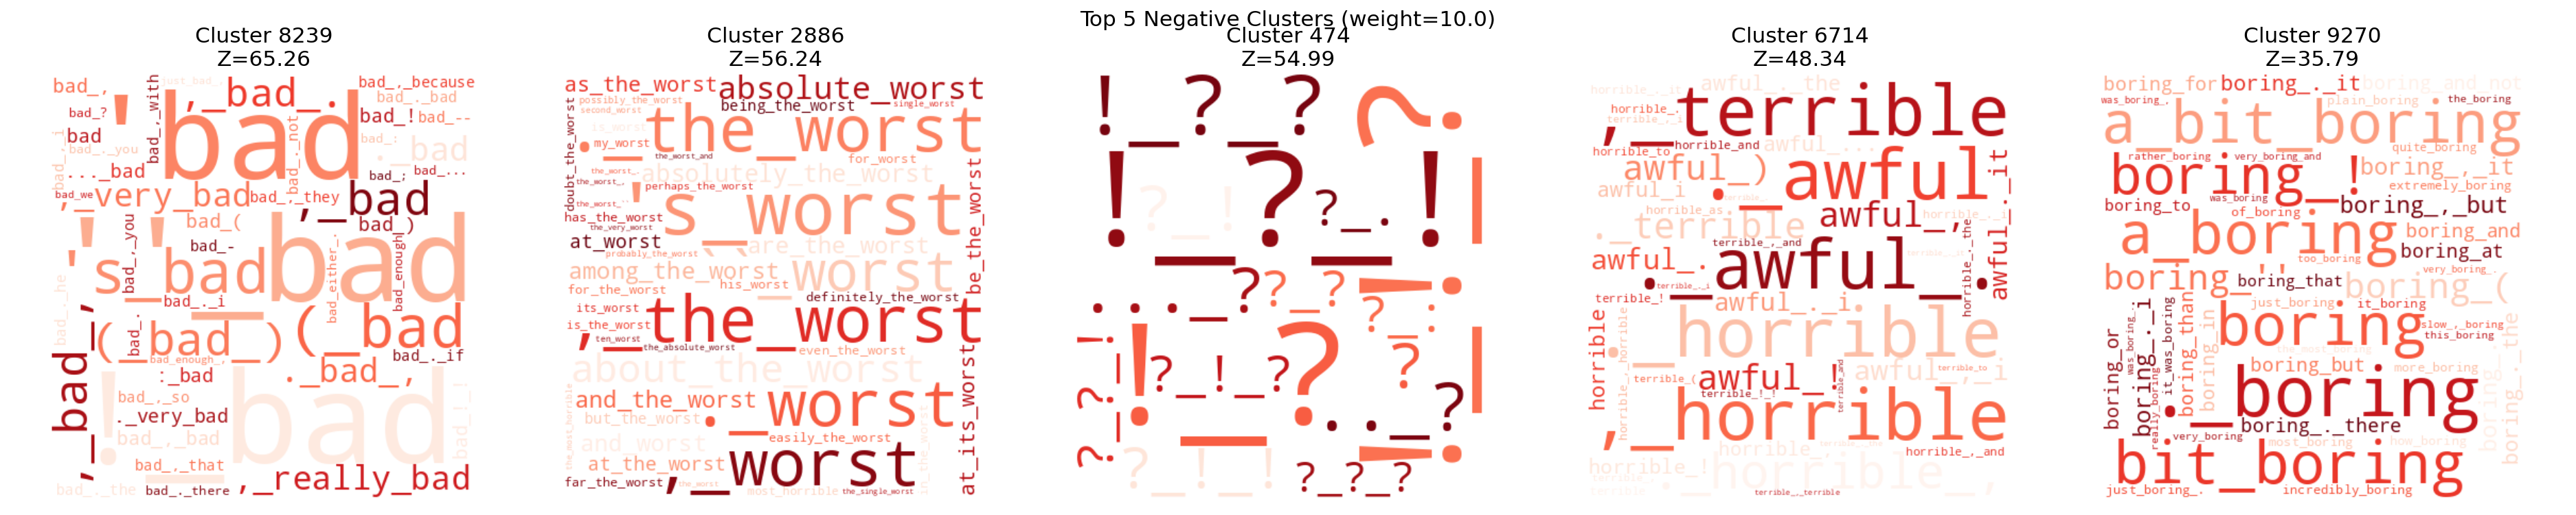
\includegraphics[width=1\textwidth]{./figures/concepts/neg_wc_tokens_lower_k10000_w10.png}
	\caption{Top 5 negative concepts extracted via weighted semantic clustering ($\conceptWeight=10$).}
	\label{fig:concepts_neg_10000_10}
\end{figure*}

\paragraph{Concept Granularity}

Compressing the vocabulary to $n$ concepts results in performance degradation for both the linear SVM and \logreg{} models. As the number of clusters increases from $\kconcepts=500$ to $\kconcepts=\num{5000}$ and $\kconcepts=\num{10000}$, the macro $F_1$-score improves, indicating that preserving nuances in vocabulary is required for effective sentiment analysis. This performance trajectory appears bounded by the benchmark; even at $\kconcepts=\num{10000}$, the clustered representations fail to surpass the unclustered baseline. Figure~\ref{fig:clustering_performance} highlights the benefit of sentiment weighting, especially at the lowest granularity ($\kconcepts=\num{500}$). Seemingly, injecting external sentiment knowledge mitigates information loss when the feature space is heavily compressed.

\begin{figure*}[tbp]%[htbp]
	\centering
	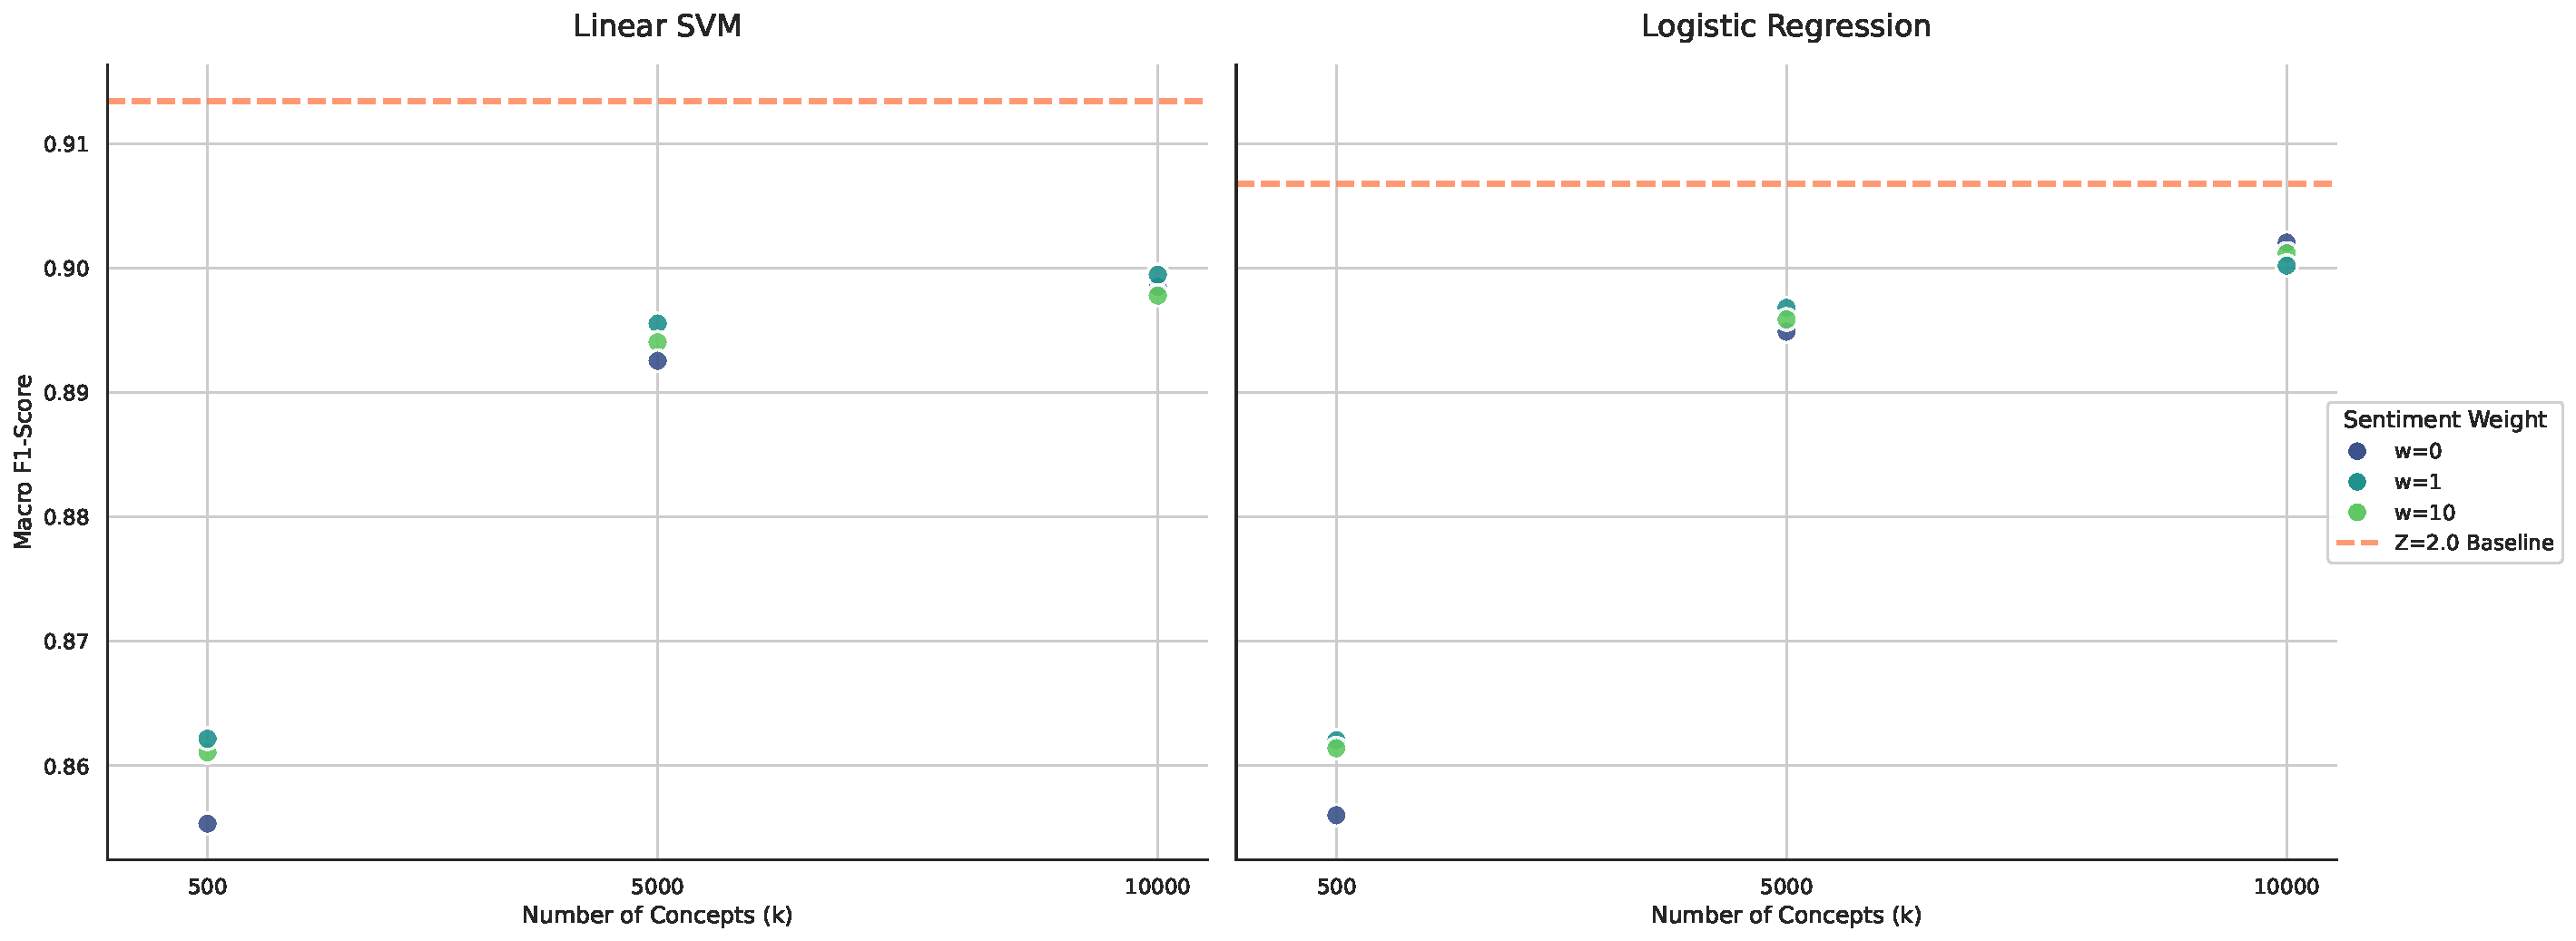
\includegraphics[width=1\textwidth]{./figures/concepts/cluster_comparison.pdf}
	\caption{Performance comparison of clustered concepts across varying  number of concepts ($\kconcepts$) and sentiment weights ($\conceptWeight$). The left and right panels detail results for the Linear SVM and \logreg{} models, respectively. Marker colors denote the applied sentiment weight ($\conceptWeight \in \{0, 1, 10\}$), while the horizontal dashed line represents the unclustered $\zscore=2.0$ baseline performance for each respective model.}
	\label{fig:clustering_performance}
\end{figure*}

\subsubsection{Impact of Certainty} \label{sec:Impact-of-Certainty}

In a cascade design the delegation decision depends on whether the predicted probability reflects genuine confidence. Figure~\ref{fig:certainty_dist} shows the probability distributions of the linear SVM and \logreg{} on the validation set. While both models concentrate predictions near the extremes, the SVM places a markedly larger share in the $[0.0,0.1]\cup[0.9,1.0]$ interval, whereas \logreg{} spreads predictions more evenly across intermediate bins.

\begin{figure*}[tbp]%[htbp]
	\centering
	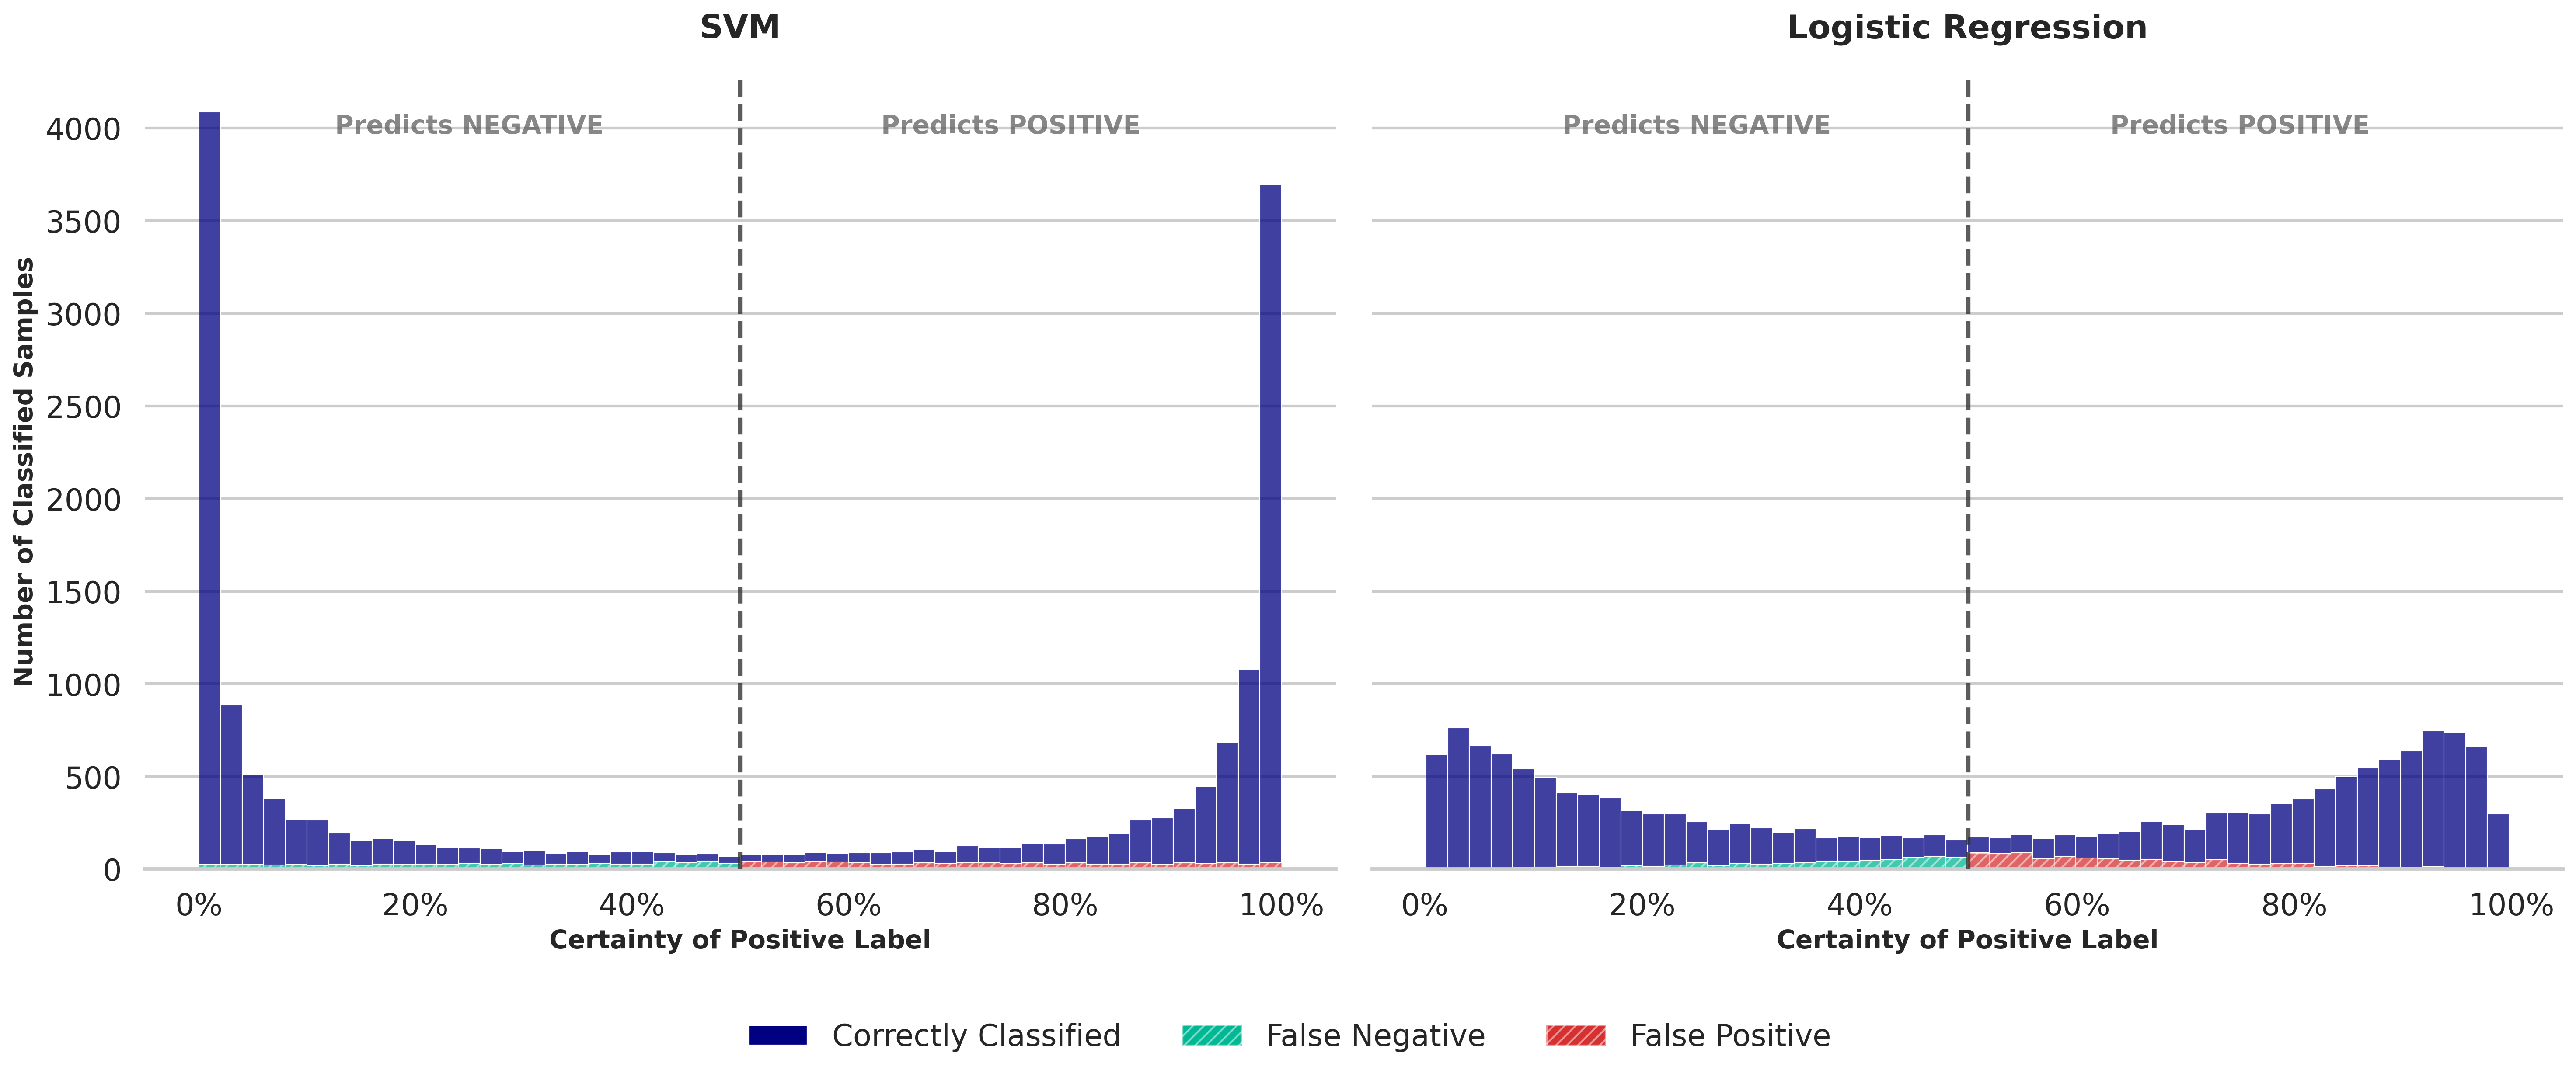
\includegraphics[width=\textwidth]{./figures/analysis/model_comparison_certainty_dist.png}
	\caption{Distribution of prediction certainty for the Linear SVM (left) and \logreg{} (right) models. The vertical dashed line at 50\% denotes the decision boundary separating negative and positive predictions. Bar colors indicate classification outcomes: dark blue represents correctly classified samples, teal indicates false negatives, and red indicates false positives.}
	\label{fig:certainty_dist}
\end{figure*}


Table~\ref{tab:certainty} partitions the probability range into five symmetric zones and reports for each zone the number of predictions, the number of misclassified samples, the local accuracy, the workload (fraction of the whole validation set falling into that zone), and the percentage of all model errors that occur specifically in that zone.

\begin{itemize}
	\item For the linear SVM, the two most certain zones alone cover $71.26\% + 11.61\% = 82.87\%$ of the data with local accuracies of $97.70\%$ and $87.10\%$, respectively. The SVM's errors, however, are distributed relatively evenly across all bins; no single interval concentrates a disproportionate share of mistakes.
	
	\item \logreg{} exhibits a pronounced error concentration in the center: $42.12\%$ of all misclassifications occur in the $[0.4,0.6]$ band, and the error share drops sharply towards the extremes (only $2.35\%$ in the outermost bin). This pattern is ideal for a cascade, because a narrow delegation window around the decision boundary would capture the bulk of the model's errors.
	
\end{itemize}

Despite this favorable error distribution, \logreg{} achieves a much smaller workload in its high-precision zone ($35.72\%$ vs.\ SVM's $71.26\%$). To match the SVM's $70\%$ coverage, three \logreg{} bins must be combined, yielding a lower average precision. The cascade therefore can benefit more from the SVM's massive high-precision coverage, using the specialist to correct the modest, spread-out errors.

\begin{table*}[tbp]%[htbp]
	\centering
	\caption{Prediction outcomes across varying certainty ranges. The tables compare the performance of the \logreg{} and SVM models, detailing the number of predictions, local accuracy, proportional workload, and relative error contribution within each symmetric probability bracket.}
	\label{tab:certainty}
	\begin{subtable}{\textwidth}
		\centering
		\caption{Certainty distribution and performance metrics for the \logreg{} model.}
		\label{tab:certainty_lr}
		\begin{tabular}{l r r r | r r}
			\toprule
			Probability Range & Predictions & Incorrect & Local Accuracy & Workload & Error \\
			\midrule
			$[0.4, 0.6]$                 & $1\,747$ & $681$ & $61.02\%$ & $10.07\%$ & $42.12\%$ \\
			$[0.3, 0.4) \cup (0.6, 0.7]$ & $2\,080$ & $443$ & $78.70\%$ & $11.99\%$ & $27.40\%$ \\
			$[0.2, 0.3) \cup (0.7, 0.8]$ & $2\,803$ & $295$ & $89.48\%$ & $16.15\%$ & $18.24\%$ \\
			$[0.1, 0.2) \cup (0.8, 0.9]$ & $4\,524$ & $160$ & $96.46\%$ & $26.07\%$ & $9.89\%$ \\
			$[0.0, 0.1) \cup (0.9, 1.0]$ & $6\,199$ & $38$ & $99.39\%$ & $35.72\%$ & $2.35\%$ \\
			\bottomrule
		\end{tabular}
	\end{subtable}
	
	\vspace{0.5em}
	
	\begin{subtable}{\textwidth}
		\centering
		\caption{Certainty distribution and performance metrics for the SVM model.}
		\label{tab:certainty_svm}
		\begin{tabular}{l r r r | r r}
			\toprule
			Certainty Range & Predictions & Incorrect & Local Accuracy & Workload & Error \\
			\midrule
			$[0.4, 0.6]$                 & $834$ & $372$ & $55.40\%$ & $4.81\%$ & $24.77\%$ \\
			$[0.3, 0.4) \cup (0.6, 0.7]$ & $929$ & $286$ & $69.21\%$ & $5.35\%$ & $19.04\%$ \\
			$[0.2, 0.3) \cup (0.7, 0.8]$ & $1\,210$ & $299$ & $75.29\%$ & $6.97\%$ & $19.91\%$ \\
			$[0.1, 0.2) \cup (0.8, 0.9]$ & $2\,015$ & $260$ & $87.10\%$ & $11.61\%$ & $17.31\%$ \\
			$[0.0, 0.1) \cup (0.9, 1.0]$ & $12\,365$ & $285$ & $97.70\%$ & $71.26\%$ & $18.97\%$ \\
			\bottomrule
		\end{tabular}
	\end{subtable}
\end{table*}

\subsubsection{Impact of Cascade Ensemble} \label{sec:Impact-of-Cascade-Ensemble}

The linear SVM cascade (Figure~\ref{fig:svm_acc_cov_trade-off}) demonstrates superior efficiency and performance when utilizing TF-IDF representations---top 4 representations can be found in the legend. The SVM begins with a high initial local accuracy (above $91.0\%$ at the $50\%$ certainty threshold) and scales smoothly to $100.0\%$ as the required confidence increases. Ultimately, the SVM cascade achieves a high overall combined accuracy, peaking at approximately $93.1\%$. Crucially, it attains this global optimization peak while delegating only $15\%$ to $20\%$ of the data to BERT. This visually confirms the earlier observation that the SVM provides a massive zone of high-precision coverage, allowing the system to rely heavily on the lightweight model without sacrificing accuracy.

\begin{figure*}[tbp]%[htbp]
	\centering
	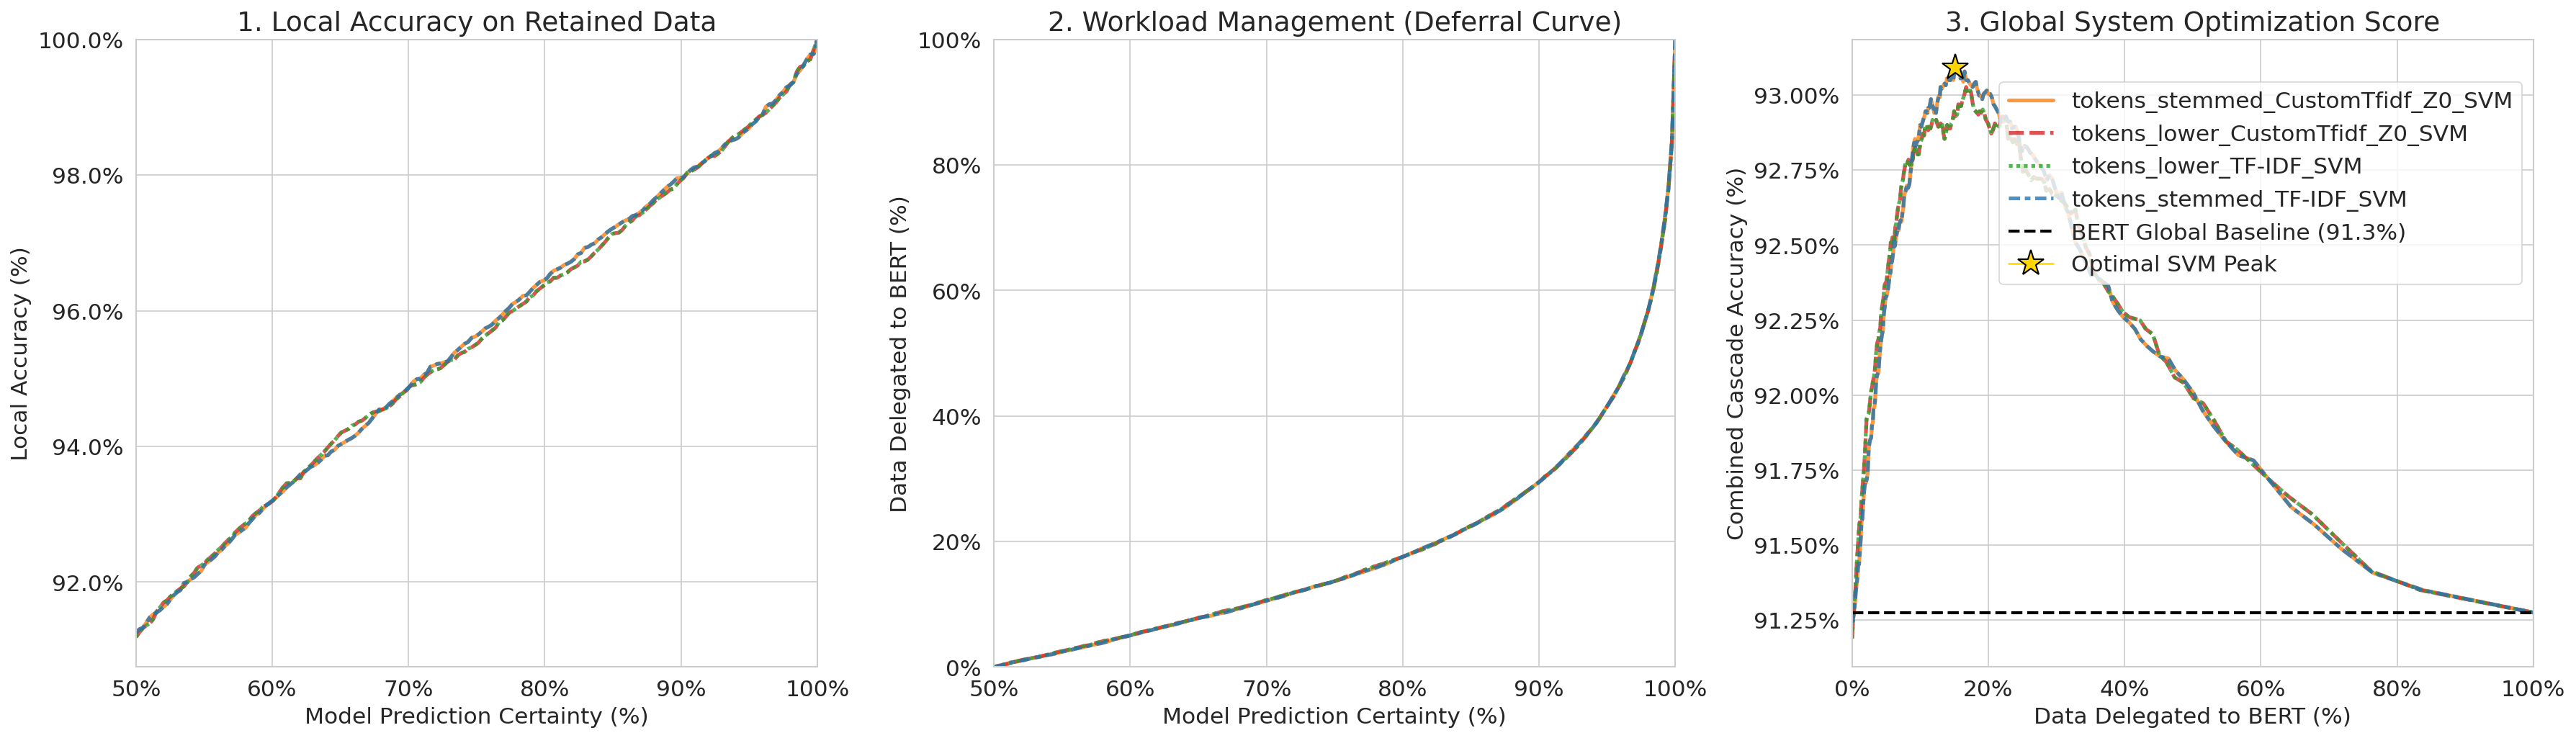
\includegraphics[width=1\textwidth]{./figures/analysis/svm_accuracy_coverage_tradeoff.png}
	\caption{Accuracy-coverage trade-off and delegation dynamics for the SVM cascade system. The left panel illustrates the local accuracy on retained data relative to the model prediction certainty threshold. The center panel presents the deferral curve, detailing the percentage of data delegated to BERT model across varying certainty thresholds. The right panel plots the combined cascade accuracy against the delegated workload, where the horizontal dashed line indicates the BERT global baseline and the star marker highlights the optimal system configuration.}
	\label{fig:svm_acc_cov_trade-off}
\end{figure*}

The \logreg{} cascade (Figure~\ref{fig:lr_acc_cov_trade-off}), predominantly utilizing BoW representations, exhibits a higher dependency on the specialist model. The local accuracy on the retained data climbs steadily from roughly $90.0\%$ to $100.0\%$ as the prediction certainty threshold increases. Consequently, the deferral curve illustrates an exponential increase in the workload delegated to BERT. While the combined cascade accuracy still significantly outperforms the BERT global baseline of $91.3\%$, reaching an optimal peak at approximately $92.9\%$ to $93.0\%$, achieving this maximum performance requires delegating roughly $25\%$ to $30\%$ of the most uncertain data to the specialist model.

\begin{figure*}[tbp]%[htbp]
	\centering
	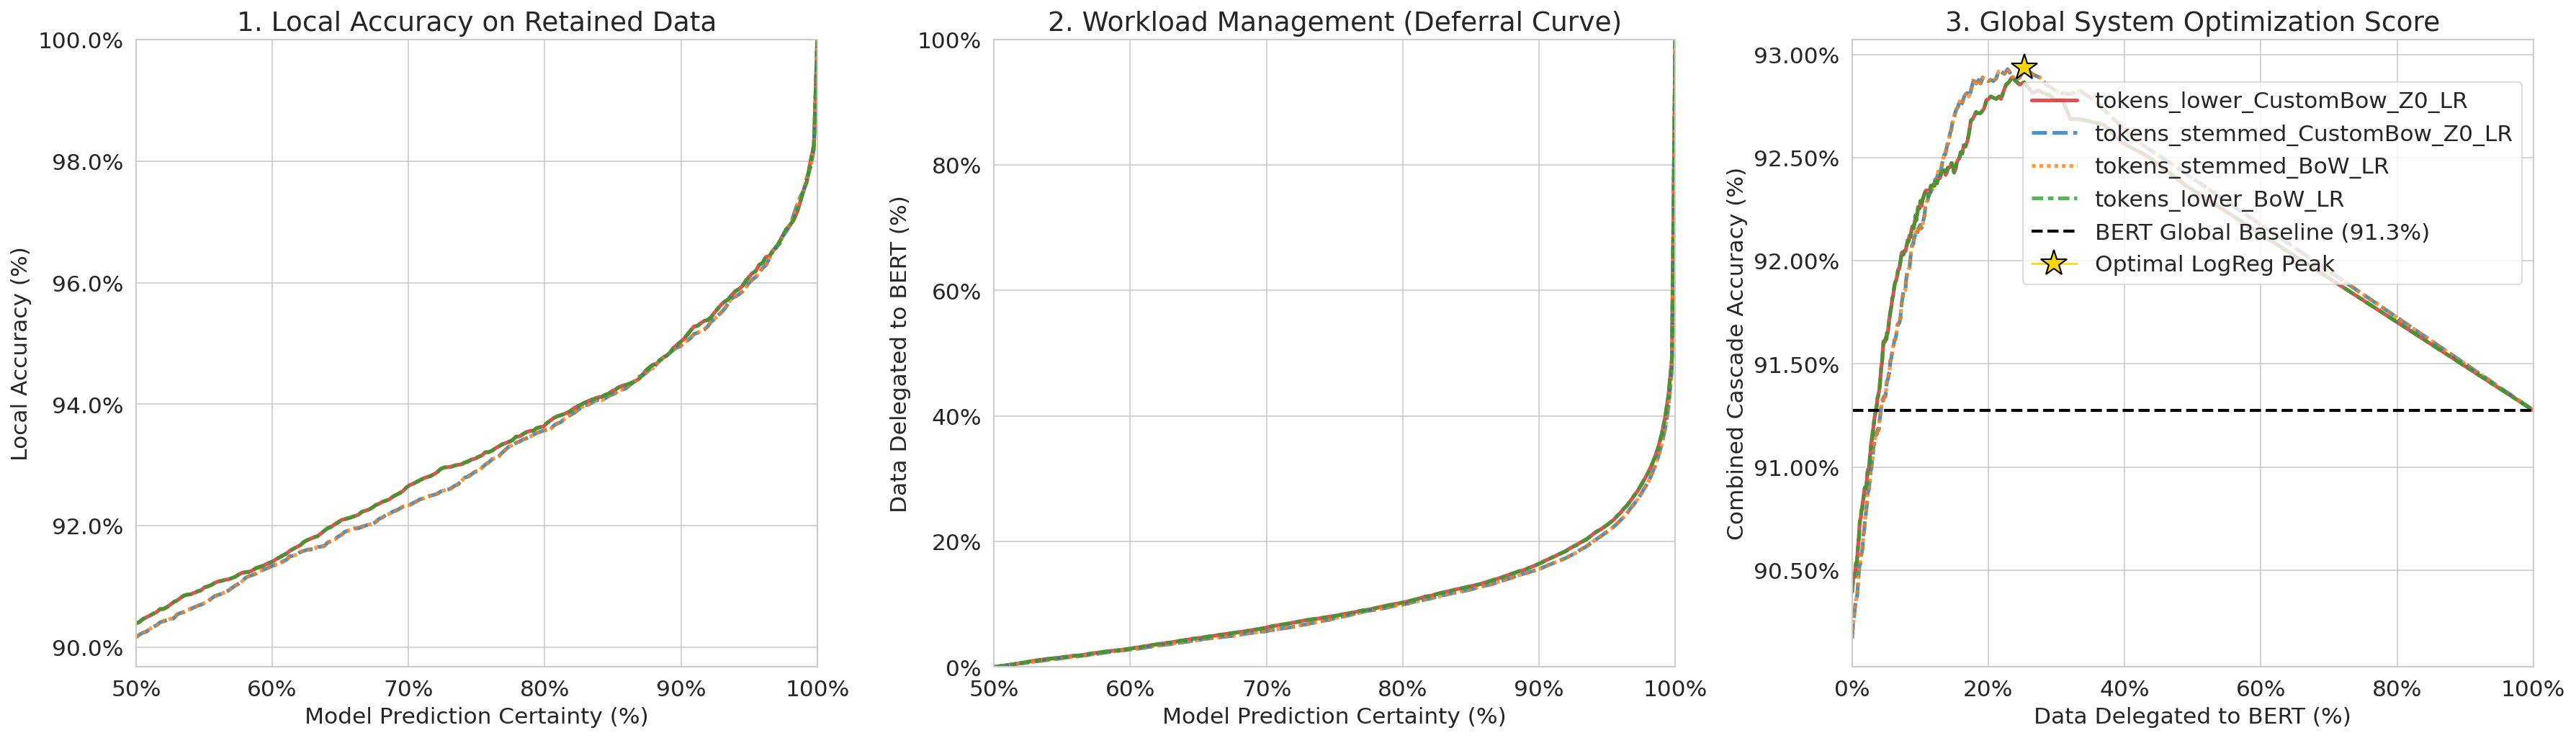
\includegraphics[width=1\textwidth]{./figures/analysis/logreg_accuracy_coverage_tradeoff.png}
	\caption{Accuracy-coverage trade-off and delegation dynamics for the \logreg{} cascade system. The left panel illustrates the local accuracy on retained data relative to the model prediction certainty threshold. The center panel presents the deferral curve, detailing the percentage of data delegated to BERT model across varying certainty thresholds. The right panel plots the combined cascade accuracy against the delegated workload, where the horizontal dashed line indicates the BERT global baseline and the star marker highlights the optimal system configuration.}
	\label{fig:lr_acc_cov_trade-off}
\end{figure*}

Overall, both configurations validate the cascade methodology, proving that deferring uncertain predictions yields better accuracy than relying on the BERT baseline alone. Nevertheless, the linear SVM cascade is markedly superior to the \logreg{} cascade, as it achieves a higher maximum accuracy while delegating significantly less data to the computationally expensive specialist model.

\paragraph{Specialist Types}

As shown in Figure~\ref{fig:cascade_comp}, introducing a specialist yields mixed results depending on its underlying mechanics---thus the choice of architecture for the specialist is crucial.

\begin{figure*}[tbp]%[htbp]
	\centering
	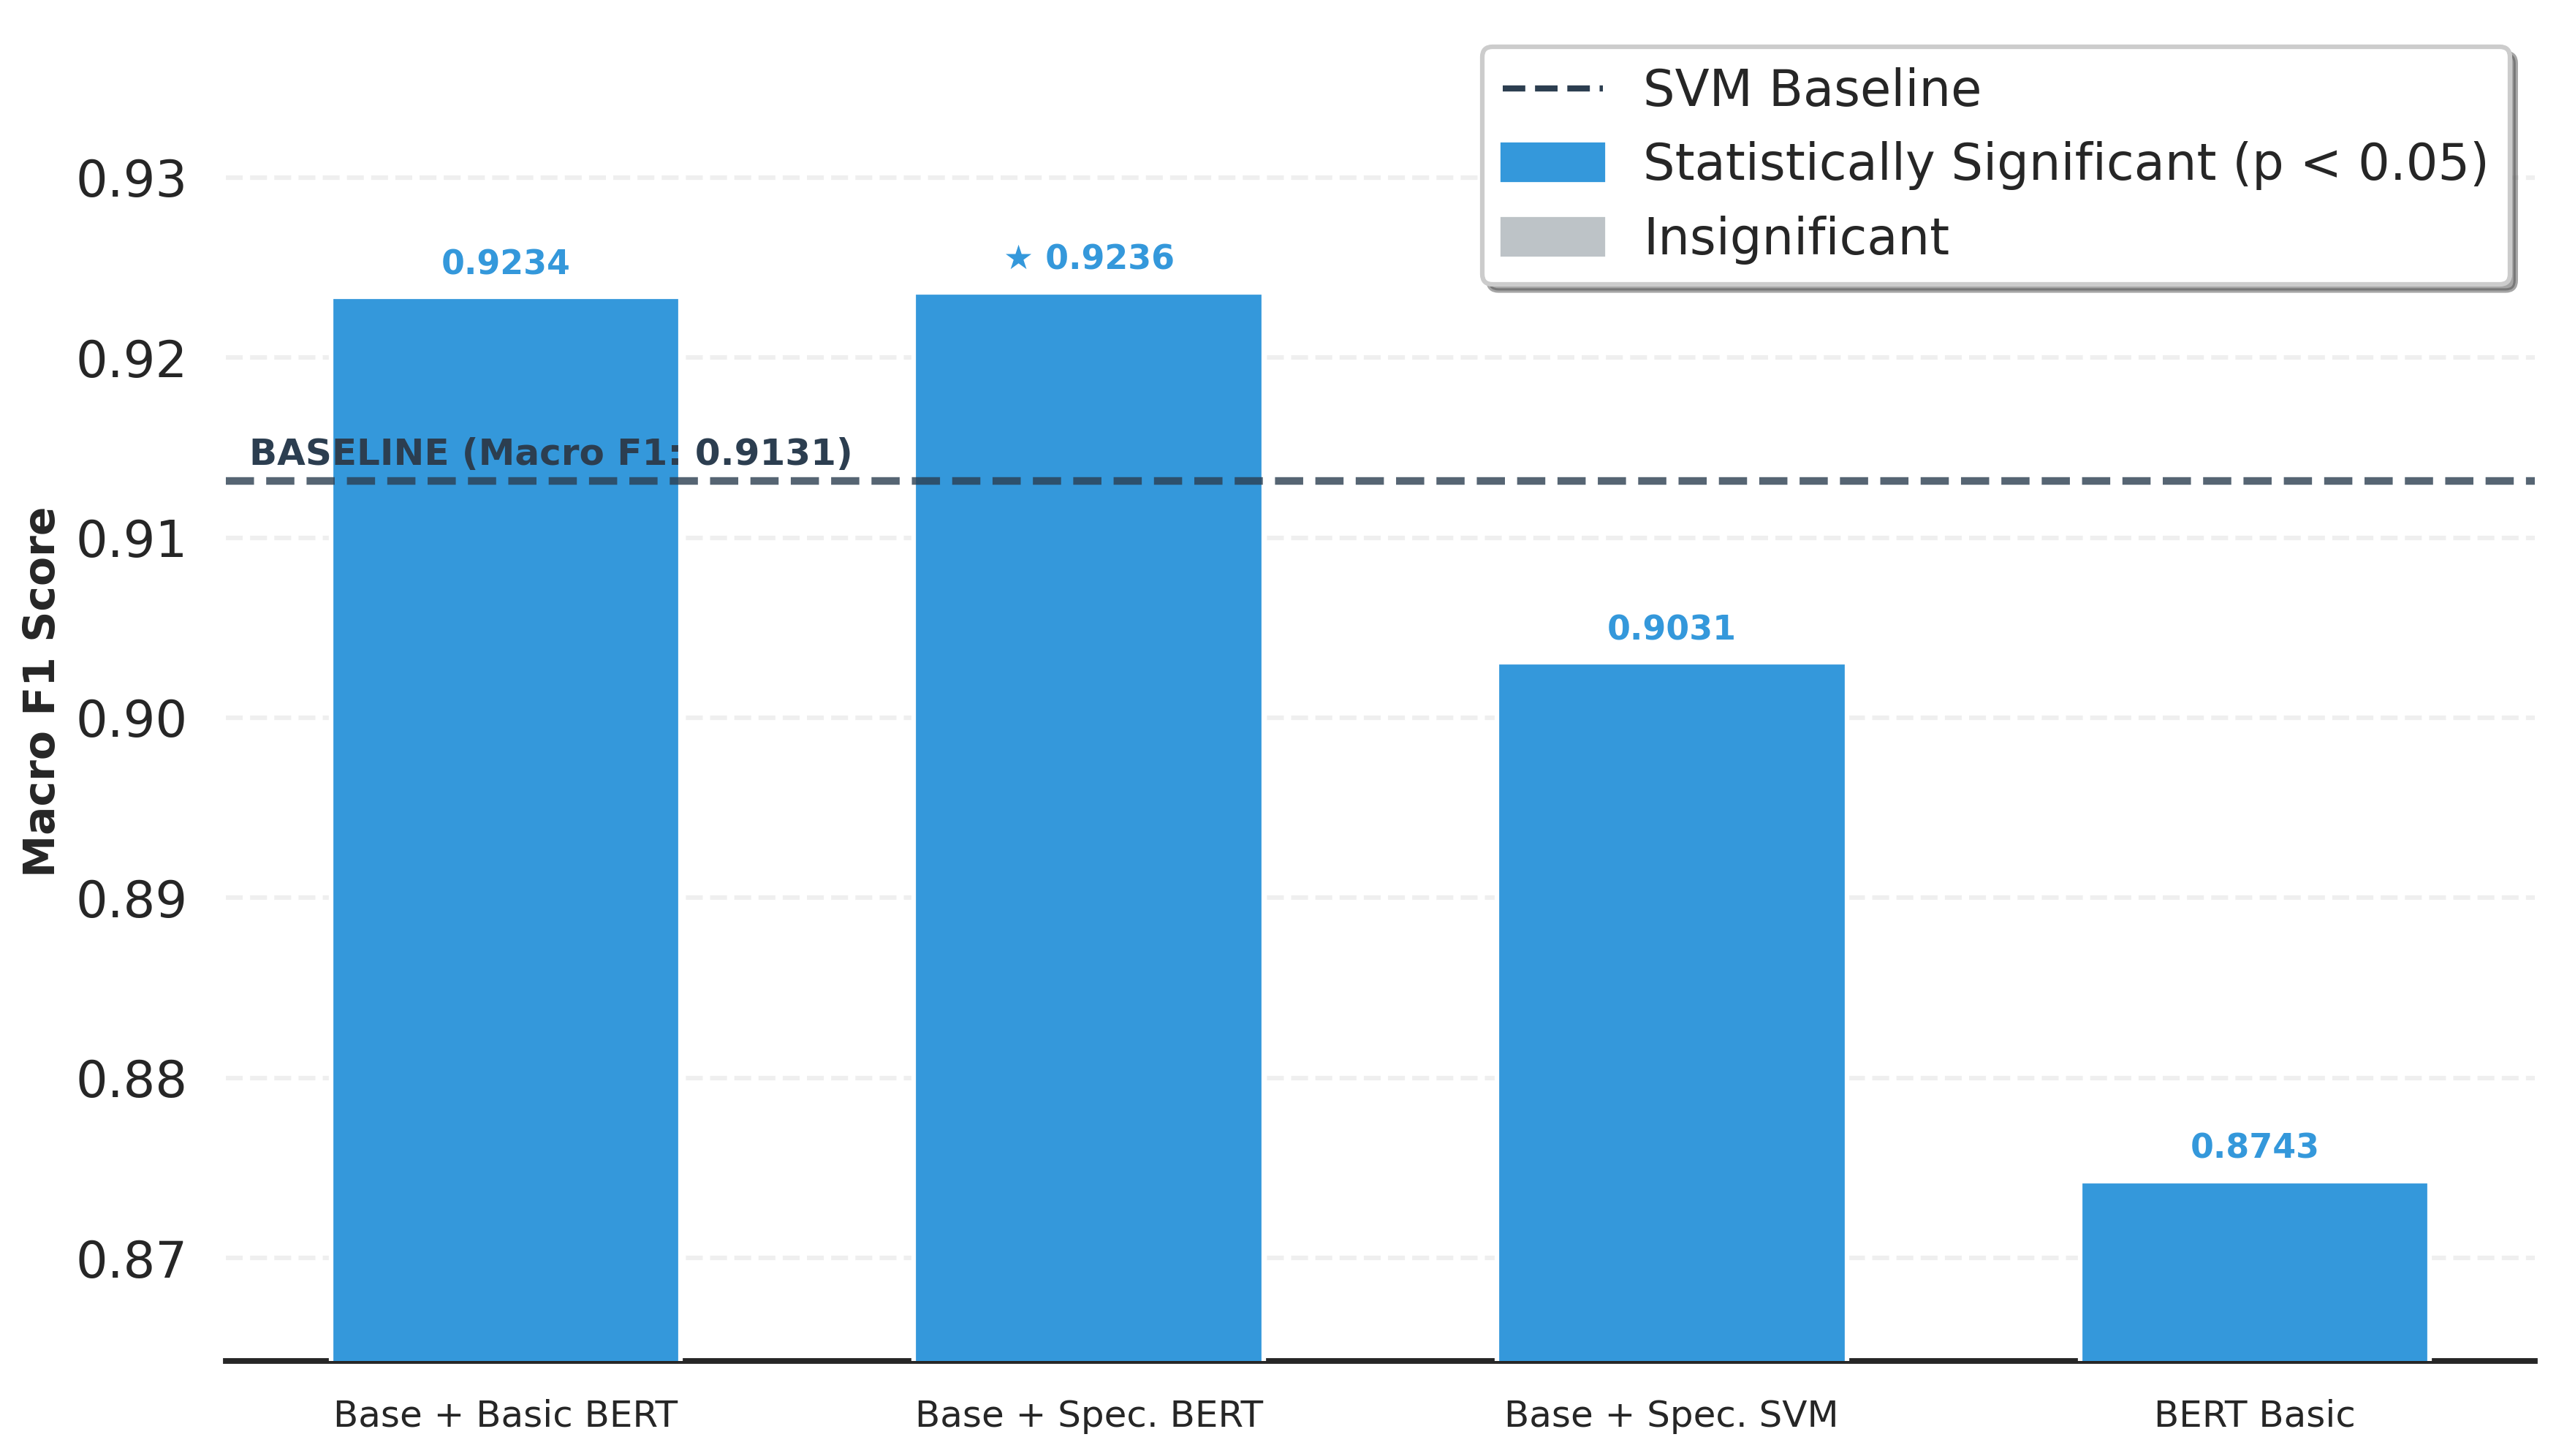
\includegraphics[width=1\textwidth]{./figures/thesis/cascade_comparison_f1_macro.png}
	\caption{Comparison of macro $F_1$-scores across different cascade system configurations. The horizontal dashed line denotes the SVM baseline performance (0.9131). Bar colors indicate statistical significance relative to the baseline (blue for $\mcnemarp < 0.05$, grey for insignificant results), and exact scores are annotated above each bar. A star marker highlights the top-performing system configuration.}
	\label{fig:cascade_comp}
\end{figure*}
\ksremark{Fig. \ref{fig:cascade_comp}: My tu nie mamy chyba Insignificant na tym rysunku, prawda?}

\begin{itemize}
	\item Both BERT cascade systems successfully surpass the SVM baseline's macro $F_1$-score of $91.31\%$. Fine-tuning a BERT specialist specifically on ``hard cases'' mined from the validation set results in a negligible performance bump over a basic BERT model ($92.36\%$ versus $92.34\%$, $p=0.859684$). This lack of statistical significance likely stems from the relatively small volume of hard samples available for fine-tuning.
	
	\item The Basic BERT model alone struggled with this specific data shuffle, achieving only an $87.43\%$ $F_1$-score on the test set, compared to its validation score of $91.27\%$. While this difficulty explains why the cascade approach dropped by almost $1\%$ overall, it highlights an interesting dynamic: combining two individually weaker models can still produce a more robust and improved overall score.
	
	\item Deploying a secondary SVM as the specialist model degrades the system's performance, dragging the macro $F_1$-score down to $0.9031$. This deterioration points to a structural limitation: the base classifier has already exploited the linear feature space. Any remaining uncertain predictions rely on subtle, highly contextual cues.
\end{itemize}

\paragraph{The Linear Limitation}

This structural barrier becomes apparent when isolating model performance strictly to the most challenging samples, as illustrated by the confusion matrices in Figure~\ref{fig:cascade_confusion}.

\begin{figure*}[tbp]%[htbp]
	\centering
	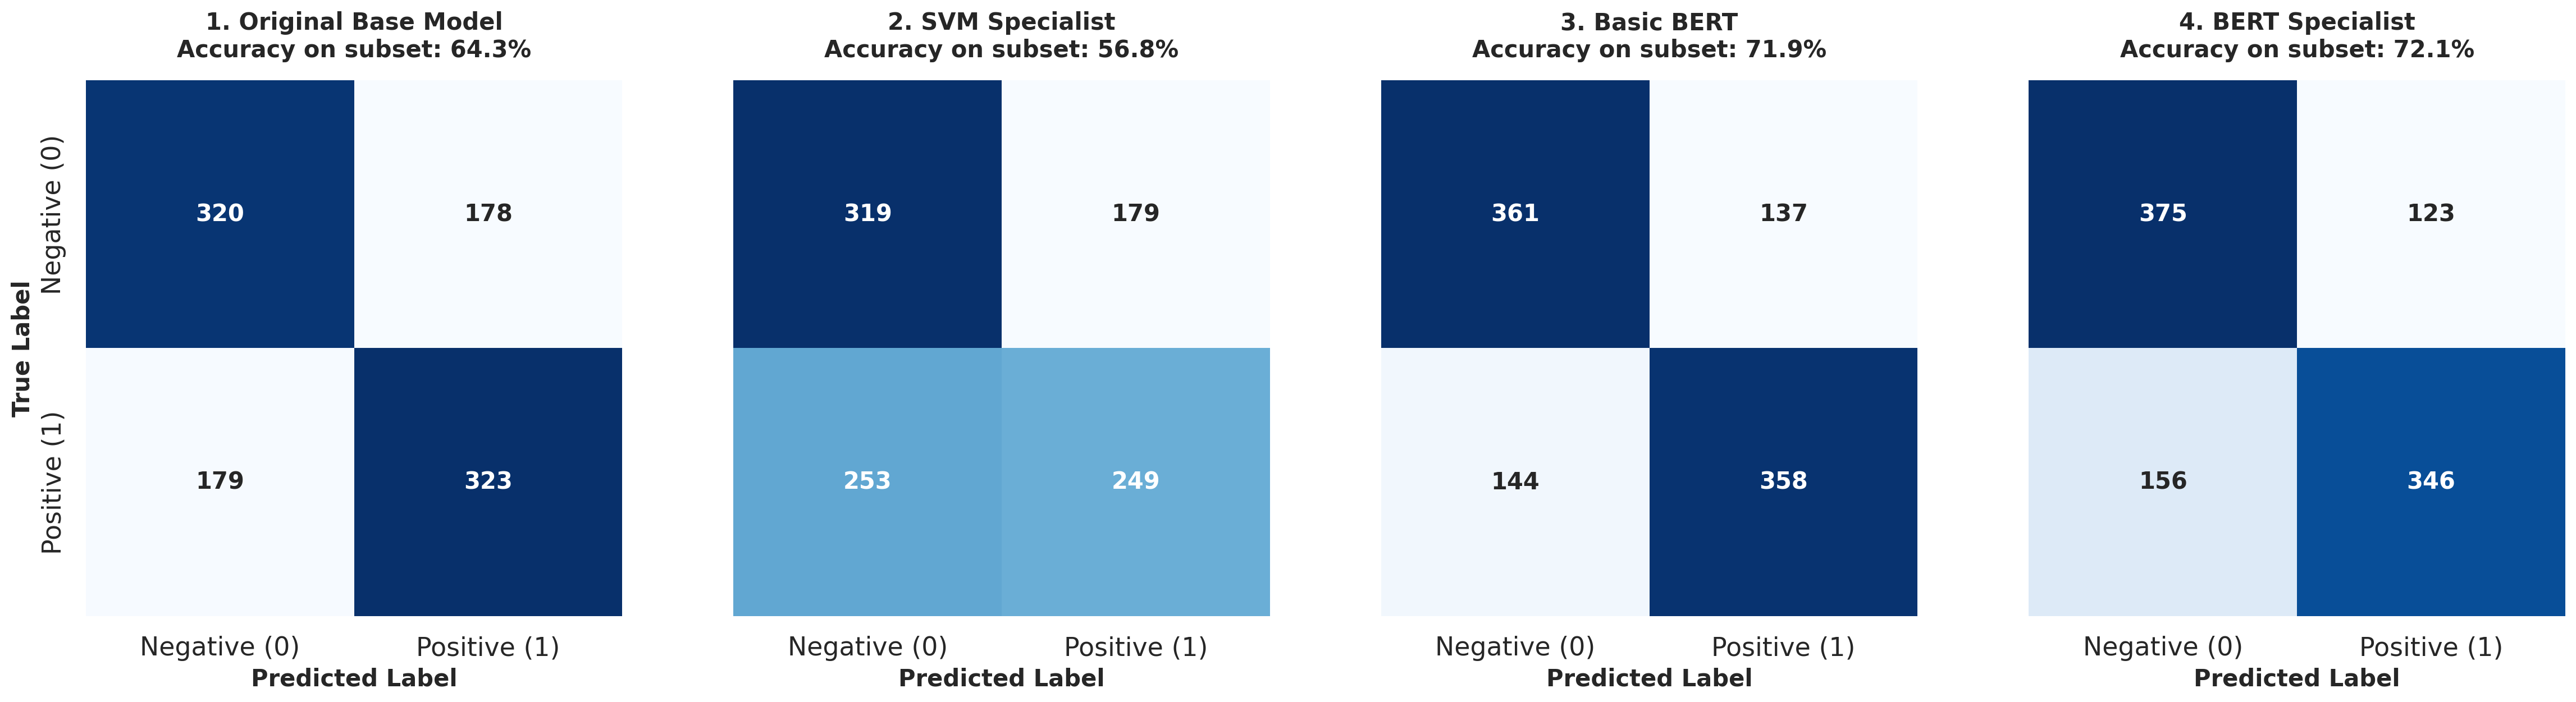
\includegraphics[width=1\textwidth]{./figures/thesis/all_models_hard_cases_cm.png}
	\caption{Confusion matrices evaluating model performance on a subset of hard samples. From left to right, the panels display the classification results for the Original Base Model, SVM Specialist, Basic BERT, and BERT Specialist. The intensity of the blue shading within each cell corresponds to the absolute number of samples, and the overall subset accuracy for each configuration is annotated above its respective matrix.}
	\label{fig:cascade_confusion}
\end{figure*}

\begin{itemize}
	\item \textbf{Base vs.\ SVM:} The original base model manages a $64.3\%$ accuracy rate on this difficult subset. When the SVM ``specialist'' attempts to re-evaluate these exact same cases, its accuracy actually plummets to $56.8\%$. This drop is primarily driven by a massive spike in false negatives, which surge from $179$ to $253$.
	
	\item \textbf{Semantic Capacity:} In sharp contrast, both BERT variants possess the deep semantic capacity necessary to untangle these non-linear, contextual cues. By successfully interpreting these complex patterns, the basic and specialist BERT models elevate the subset accuracy to $71.9\%$ and $72.1\%$, respectively.
\end{itemize}




\section{Summary} \label{chap:summary}

\subsection{Motivation and Objective}

Sentiment analysis is a well-established NLP task, yet a persistent trade‑off remains between the high accuracy of modern deep learning models and the computational efficiency required for practical deployment. This thesis investigated whether GrC techniques can bridge this gap.

\subsection{Summary of Work}

Granular computing approaches had not been systematically verified in the sentiment analysis pipeline. Through an enumeration of preprocessing, representation, and modeling choices, the most effective configurations were identified. The work demonstrated that a statistical $\zscore$-based pruning technique can discard the ``neutral'' granule---the $n$-grams that do not discriminate between positive and negative classes---thereby reducing the feature space while preserving or even improving accuracy. Building on this, a hybrid cascade ensemble was proposed: a lightweight linear SVM acts as a base model, handling the majority of instances with high confidence, while a deep learning specialist (DistilBERT) resolves the remaining uncertain cases. The cascade achieved a macro $F_1$-score of approximately $92.3\%$, outperforming both standalone baselines while delegating only $15\%$-$20\%$ of the data to the expensive model.

\subsection{Conclusions}

The positive aspects of the proposed approaches are lower computational cost and less sparse feature spaces. Most of the workload can be handled by the baseline SVM model, while only a small fraction of the most difficult instances is passed to the specialist. This division of labor combines efficiency with high accuracy and demonstrates that granular principles can successfully guide the design of a practical sentiment analysis system.

\subsubsection{Recommendations}

\begin{itemize}
	\item \textbf{Preprocessing is necessary, and data unification is important.} Text should be at least lowercased and expanded (contraction resolution) to ensure better generalization when using traditional machine learning approaches. Stemming and lemmatization do not significantly improve or degrade accuracy and may be omitted.
	
	\item \textbf{POS-based filtering (stop-word removal) is not advised.} Although it reduces the feature space, it imposes a ceiling on performance and is not among the best-performing representations for SVM.
	
	\item \textbf{SVMs are a much better choice than \logreg{} as baseline models.} SVMs achieve higher standalone accuracy and, critically, separate easy from difficult cases more effectively, making them more suitable for cascade architectures. 
	\item \textbf{The linear kernel is fast and reliable.} The RBF kernel trains much longer and does not converge in an acceptable time, while offering no accuracy benefit.
	
	\item \textbf{Custom Bag-of-Words (BoW) does not benefit from pruning, but $\mathbf{\zscore}$-based pruning works well with TF-IDF.} A pruning threshold of $\zscore = 2.0$ retains or even improves accuracy while discarding over $60\%$ of the feature space.
	
	\item \textbf{There is no statistically significant difference between $\mathbf{(1,2)}$-grams and $\mathbf{(1,3)}$-grams.} Unigrams alone are not enough to capture sufficient understanding.
	
	
	\item \textbf{Semantic clustering works for topic classification, but is not useful for SA.} Even when external sentiment values are injected, concept-level representations erase too many polarity cues and underperform token-level features.
	
	\item \textbf{The cascade ensemble works better than expected.} Because the SVM and the transformer model operate on different feature spaces, they learn complementary aspects: the SVM handles the separation of easy from difficult cases, while the transformer focuses on understanding nuanced, contextual sentiment. The cascade achieves better results than DistilBERT or SVM baselines alone. An SVM cannot be used as a specialist because the remaining ambiguities are not resolvable within a pure vectorized (BoW or TF-IDF) representation.
	
	\item \textbf{Cascade systems can reliably use a separate validation set to establish the optimal deferral rate.} The threshold selected on held-out data generalizes well to unseen test data.
\end{itemize}

\subsubsection{Research Questions Revisited}

\subparagraph{RQ1:} \emph{Can granular approaches be used to optimize the sentiment analysis pipeline?}

Yes. Statistical pruning based on $\zscore$-scores works effectively: the ``not sentiment’’ granule is discarded, leading to a more compact and equally or more accurate feature representation.

\subparagraph{RQ2:} \emph{Can a hybrid system be designed to combine the efficiency of lightweight classifiers with the semantic understanding of transformer models?}

Yes. A cascade ensemble can be built that improves overall performance, with the base SVM handling the majority of instances and the specialist transformer resolving only the hardest cases.

\subsubsection{Further Research}

Further research could verify whether higher-order $n$-grams (e.g., $(1,4)$ and beyond) become feasible when combined with the proposed statistical pruning approach.

It should also be tested whether stronger models---full BERT or LLMs---could benefit from a cascade, saving inference tokens by deferring only a small fraction of instances to the heavyweight model; it is possible that such models are already so strong that the cascade would weaken their performance.

Another direction is to test whether semantic clustering could be applied at the sentence level, where similar sentences are grouped into prototypical concepts. This would require a specialized classifier that maps a sentence to its concept representative, since the set of possible sentences is unlimited and a static mapping matrix---as used here for $n$-grams---would not be possible.


%\subsection{Introduction}
%
%The Elsevier cas-dc class is based on the
%standard article class and supports almost all of the functionality of
%that class. In addition, it features commands and options to format the
%\begin{itemize} \item document style \item baselineskip \item front
%matter \item keywords and MSC codes \item theorems, definitions and
%proofs \item lables of enumerations \item citation style and labeling.
%\end{itemize}
%
%This class depends on the following packages
%for its proper functioning:
%
%\begin{enumerate}
%\itemsep=0pt
%\item {natbib.sty} for citation processing;
%\item {geometry.sty} for margin settings;
%\item {fleqn.clo} for left aligned equations;
%\item {graphicx.sty} for graphics inclusion;
%\item {hyperref.sty} optional packages if hyperlinking is
%  required in the document;
%\end{enumerate}  
%
%All the above packages are part of any
%standard \LaTeX{} installation.
%Therefore, the users need not be
%bothered about downloading any extra packages.
%
%\subsection{Installation}
%
%The package is available at author resources page at Elsevier
%(\url{http://www.elsevier.com/locate/latex}).
%The class may be moved or copied to a place, usually,\linebreak
%\verb+$TEXMF/tex/latex/elsevier/+, %$%%%%%%%%%%%%%%%%%%%%%%%%%%%%
%or a folder which will be read                   
%by \LaTeX{} during document compilation.  The \TeX{} file
%database needs updation after moving/copying class file.  Usually,
%we use commands like \verb+mktexlsr+ or \verb+texhash+ depending
%upon the distribution and operating system.
%
%\subsection{Front matter}
%
%The author names and affiliations could be formatted in two ways:
%\begin{enumerate}[(1)]
%\item Group the authors per affiliation.
%\item Use footnotes to indicate the affiliations.
%\end{enumerate}
%See the front matter of this document for examples. 
%You are recommended to conform your choice to the journal you 
%are submitting to.
%
%\subsection{Bibliography styles}
%
%There are various bibliography styles available. You can select the
%style of your choice in the preamble of this document. These styles are
%Elsevier styles based on standard styles like Harvard and Vancouver.
%Please use Bib\TeX\ to generate your bibliography and include DOIs
%whenever available.
%
%Here are two sample references: 
%\cite{Fortunato2010}
%\cite{Fortunato2010,NewmanGirvan2004}
%\cite{Fortunato2010,Vehlowetal2013}
%
%\subsection{Floats}
%{Figures} may be included using the command,\linebreak 
%\verb+\includegraphics+ in
%combination with or without its several options to further control
%graphic. \verb+\includegraphics+ is provided by {graphic[s,x].sty}
%which is part of any standard \LaTeX{} distribution.
%{graphicx.sty} is loaded by default. \LaTeX{} accepts figures in
%the postscript format while pdf\LaTeX{} accepts {*.pdf},
%{*.mps} (metapost), {*.jpg} and {*.png} formats. 
%pdf\LaTeX{} does not accept graphic files in the postscript format. 
%
%\begin{figure}
%	\centering
%	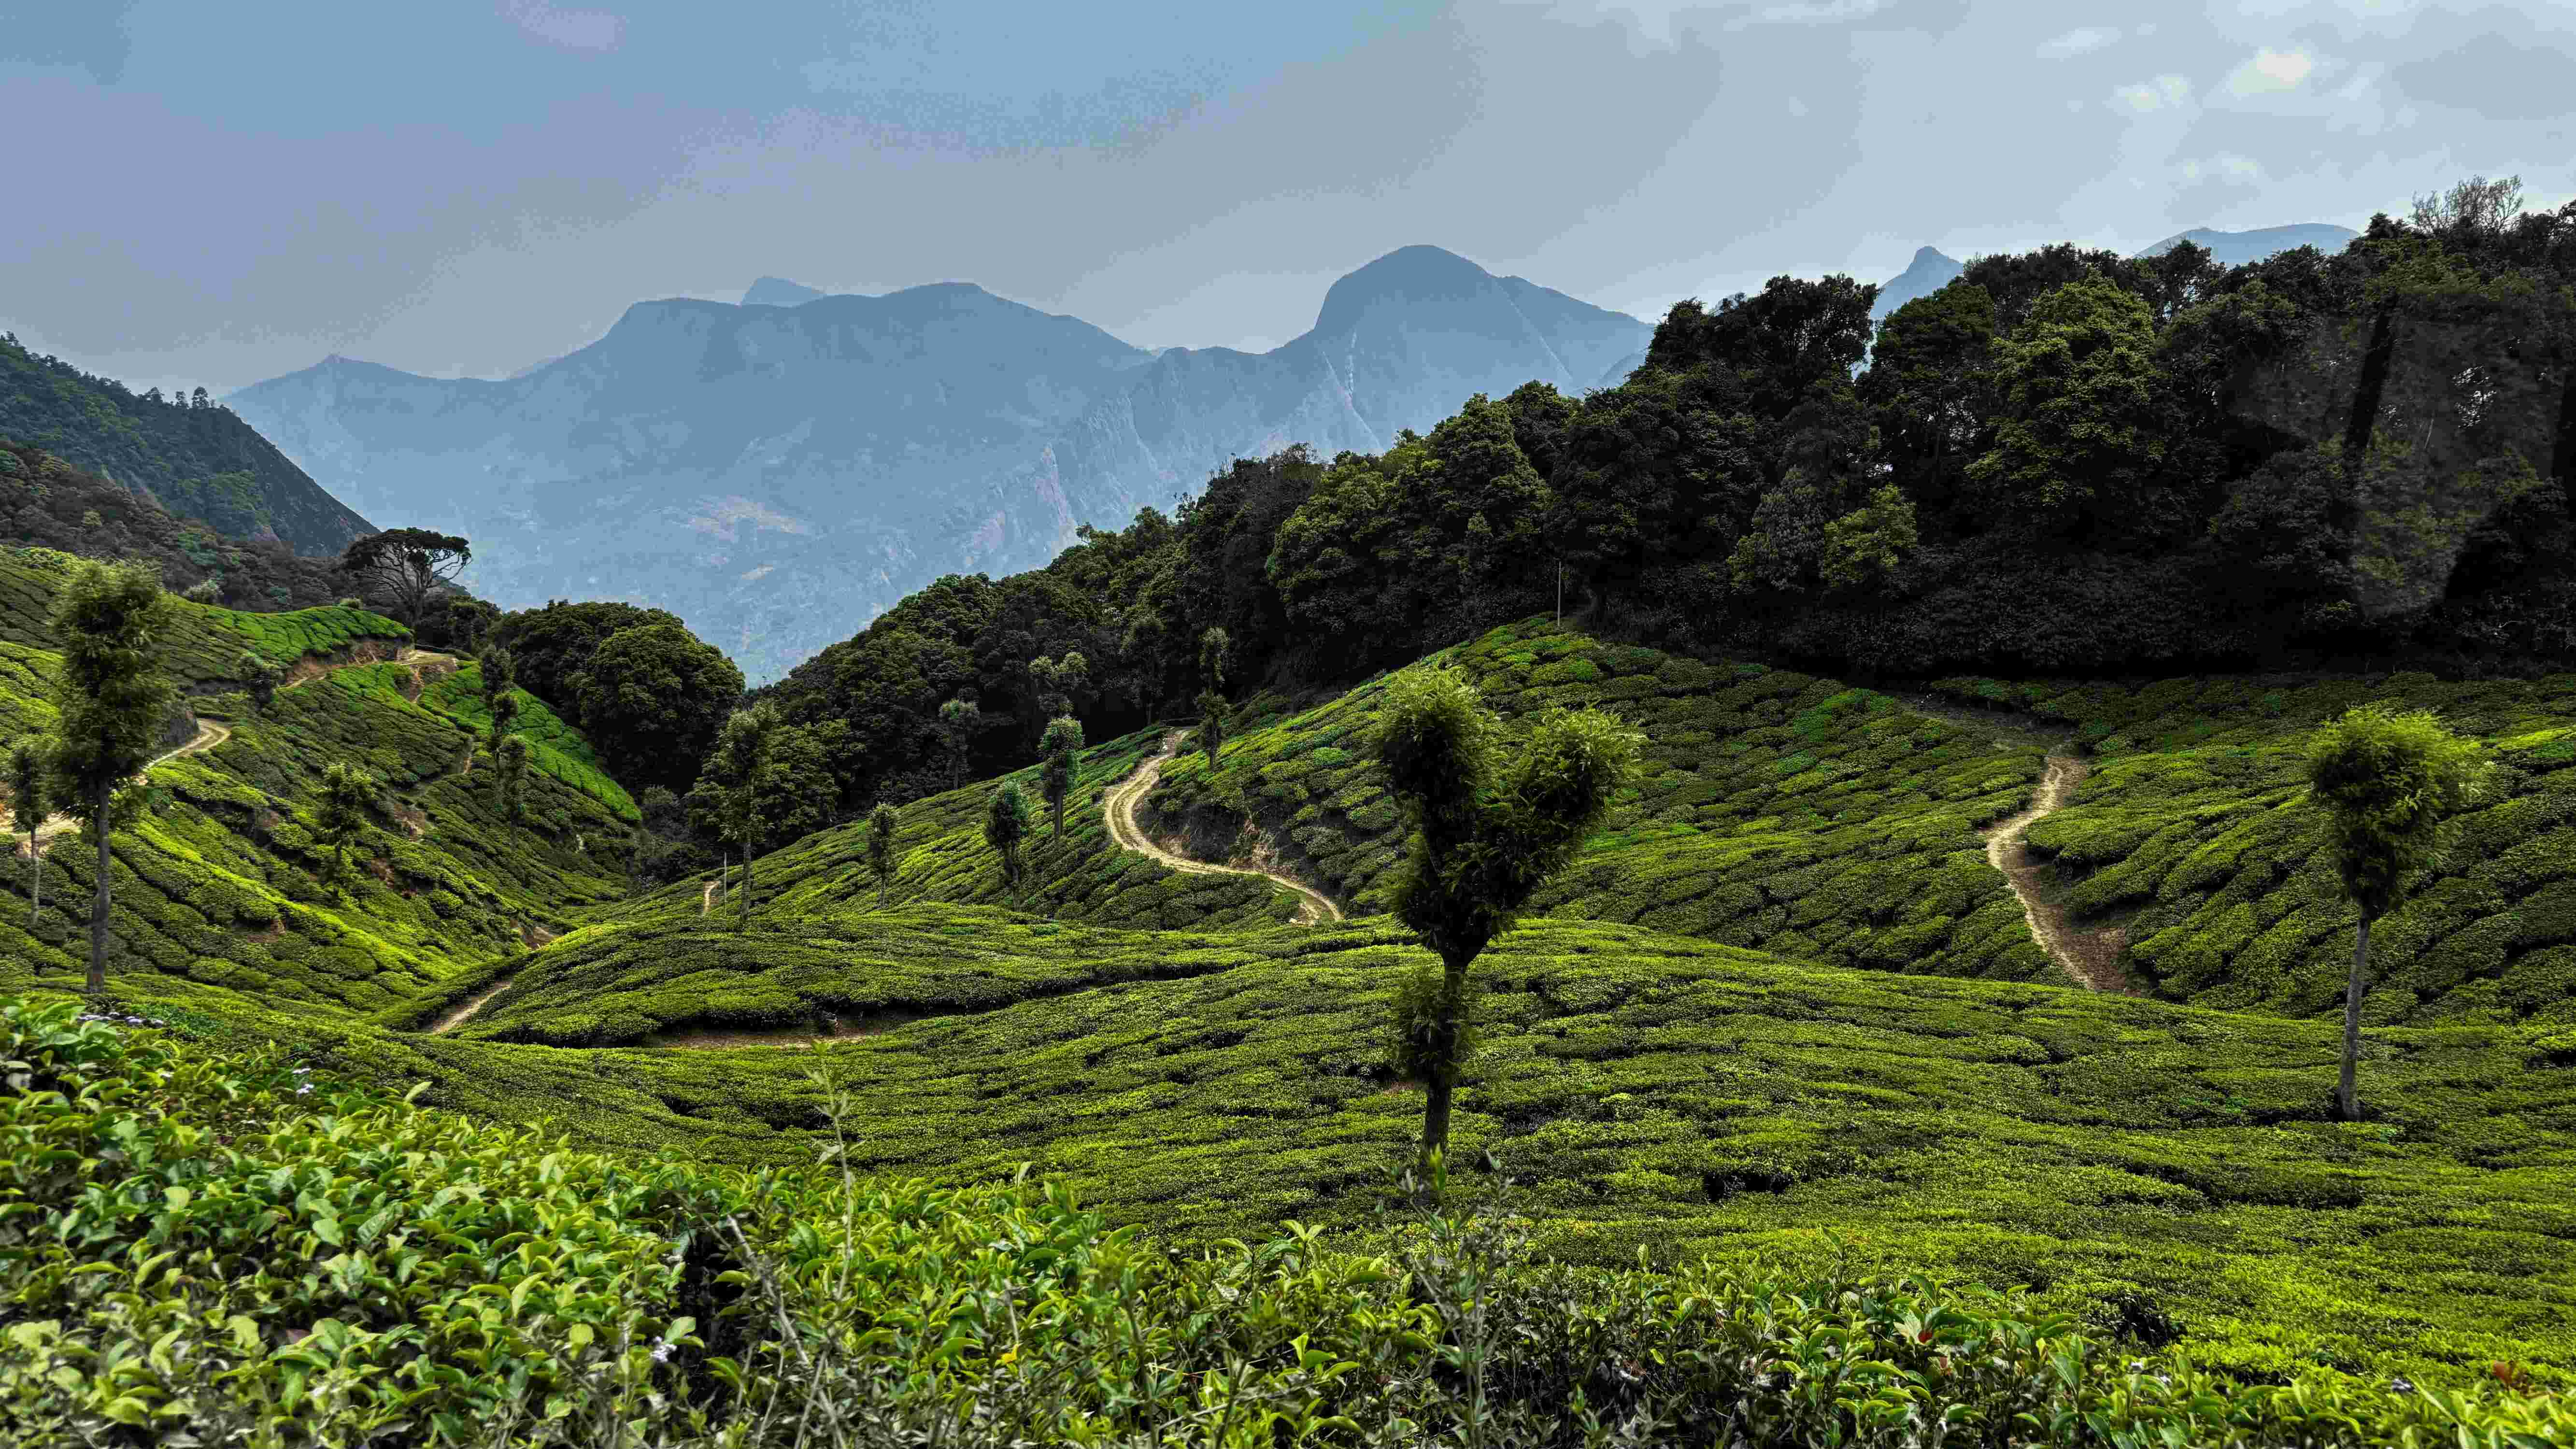
\includegraphics[width=.9\columnwidth]{figs/cas-munnar-2024.jpg}
%	\caption{The beauty of Munnar, Kerala. (See also Table \protect\ref{tbl1}).}
%	\label{FIG:1}
%\end{figure}
%
%
%The \verb+table+ environment is handy for marking up tabular
%material. If users want to use {multirow.sty},
%{array.sty}, etc., to fine control/enhance the tables, they
%are welcome to load any package of their choice and
%{cas-dc.cls} will work in combination with all loaded
%packages.
%
%\begin{table}[width=.9\linewidth,cols=4,pos=h]
%\caption{This is a test caption. This is a test caption. This is a test
%caption. This is a test caption. Use \{table*\} instead of \{table\} if you
%want a two column spanned table.}\label{tbl1}
%\begin{tabular*}{\tblwidth}{@{} LLLL@{} }
%\toprule
%Col 1 & Col 2 & Col 3 & Col4\\
%\midrule
%12345 & 12345 & 123 & 12345 \\
%12345 & 12345 & 123 & 12345 \\
%12345 & 12345 & 123 & 12345 \\
%12345 & 12345 & 123 & 12345 \\
%12345 & 12345 & 123 & 12345 \\
%\bottomrule
%\end{tabular*}
%\end{table}
%
%\subsection[Theorem and ...]{Theorem and theorem like environments}
%
%{cas-dc.cls} provides a few shortcuts to format theorems and
%theorem-like environments with ease. In all commands the options that
%are used with the \verb+\newtheorem+ command will work exactly in the same
%manner. {cas-dc.cls} provides three commands to format theorem or
%theorem-like environments: 
%
%\begin{verbatim}
% \newtheorem{theorem}{Theorem}
% \newtheorem{lemma}[theorem]{Lemma}
% \newdefinition{rmk}{Remark}
% \newproof{pf}{Proof}
% \newproof{pot}{Proof of Theorem \ref{thm2}}
%\end{verbatim}
%
%
%The \verb+\newtheorem+ command formats a
%theorem in \LaTeX's default style with italicized font, bold font
%for theorem heading and theorem number at the right hand side of the
%theorem heading.  It also optionally accepts an argument which
%will be printed as an extra heading in parentheses. 
%
%\begin{verbatim}
%  \begin{theorem} 
%   For system (8), consensus can be achieved with 
%   $\|T_{\omega z}$ ...
%     \begin{eqnarray}\label{10}
%     ....
%     \end{eqnarray}
%  \end{theorem}
%\end{verbatim}  
%
%
%\newtheorem{theorem}{Theorem}
%
%\begin{theorem}
%For system (8), consensus can be achieved with 
%$\|T_{\omega z}$ ...
%\begin{eqnarray}\label{10}
%....
%\end{eqnarray}
%\end{theorem}
%
%The \verb+\newdefinition+ command is the same in
%all respects as its \verb+\newtheorem+ counterpart except that
%the font shape is roman instead of italic.  Both
%\verb+\newdefinition+ and \verb+\newtheorem+ commands
%automatically define counters for the environments defined.
%
%The \verb+\newproof+ command defines proof environments with
%upright font shape.  No counters are defined. 
%
%\begin{figure*}
%	\centering
%	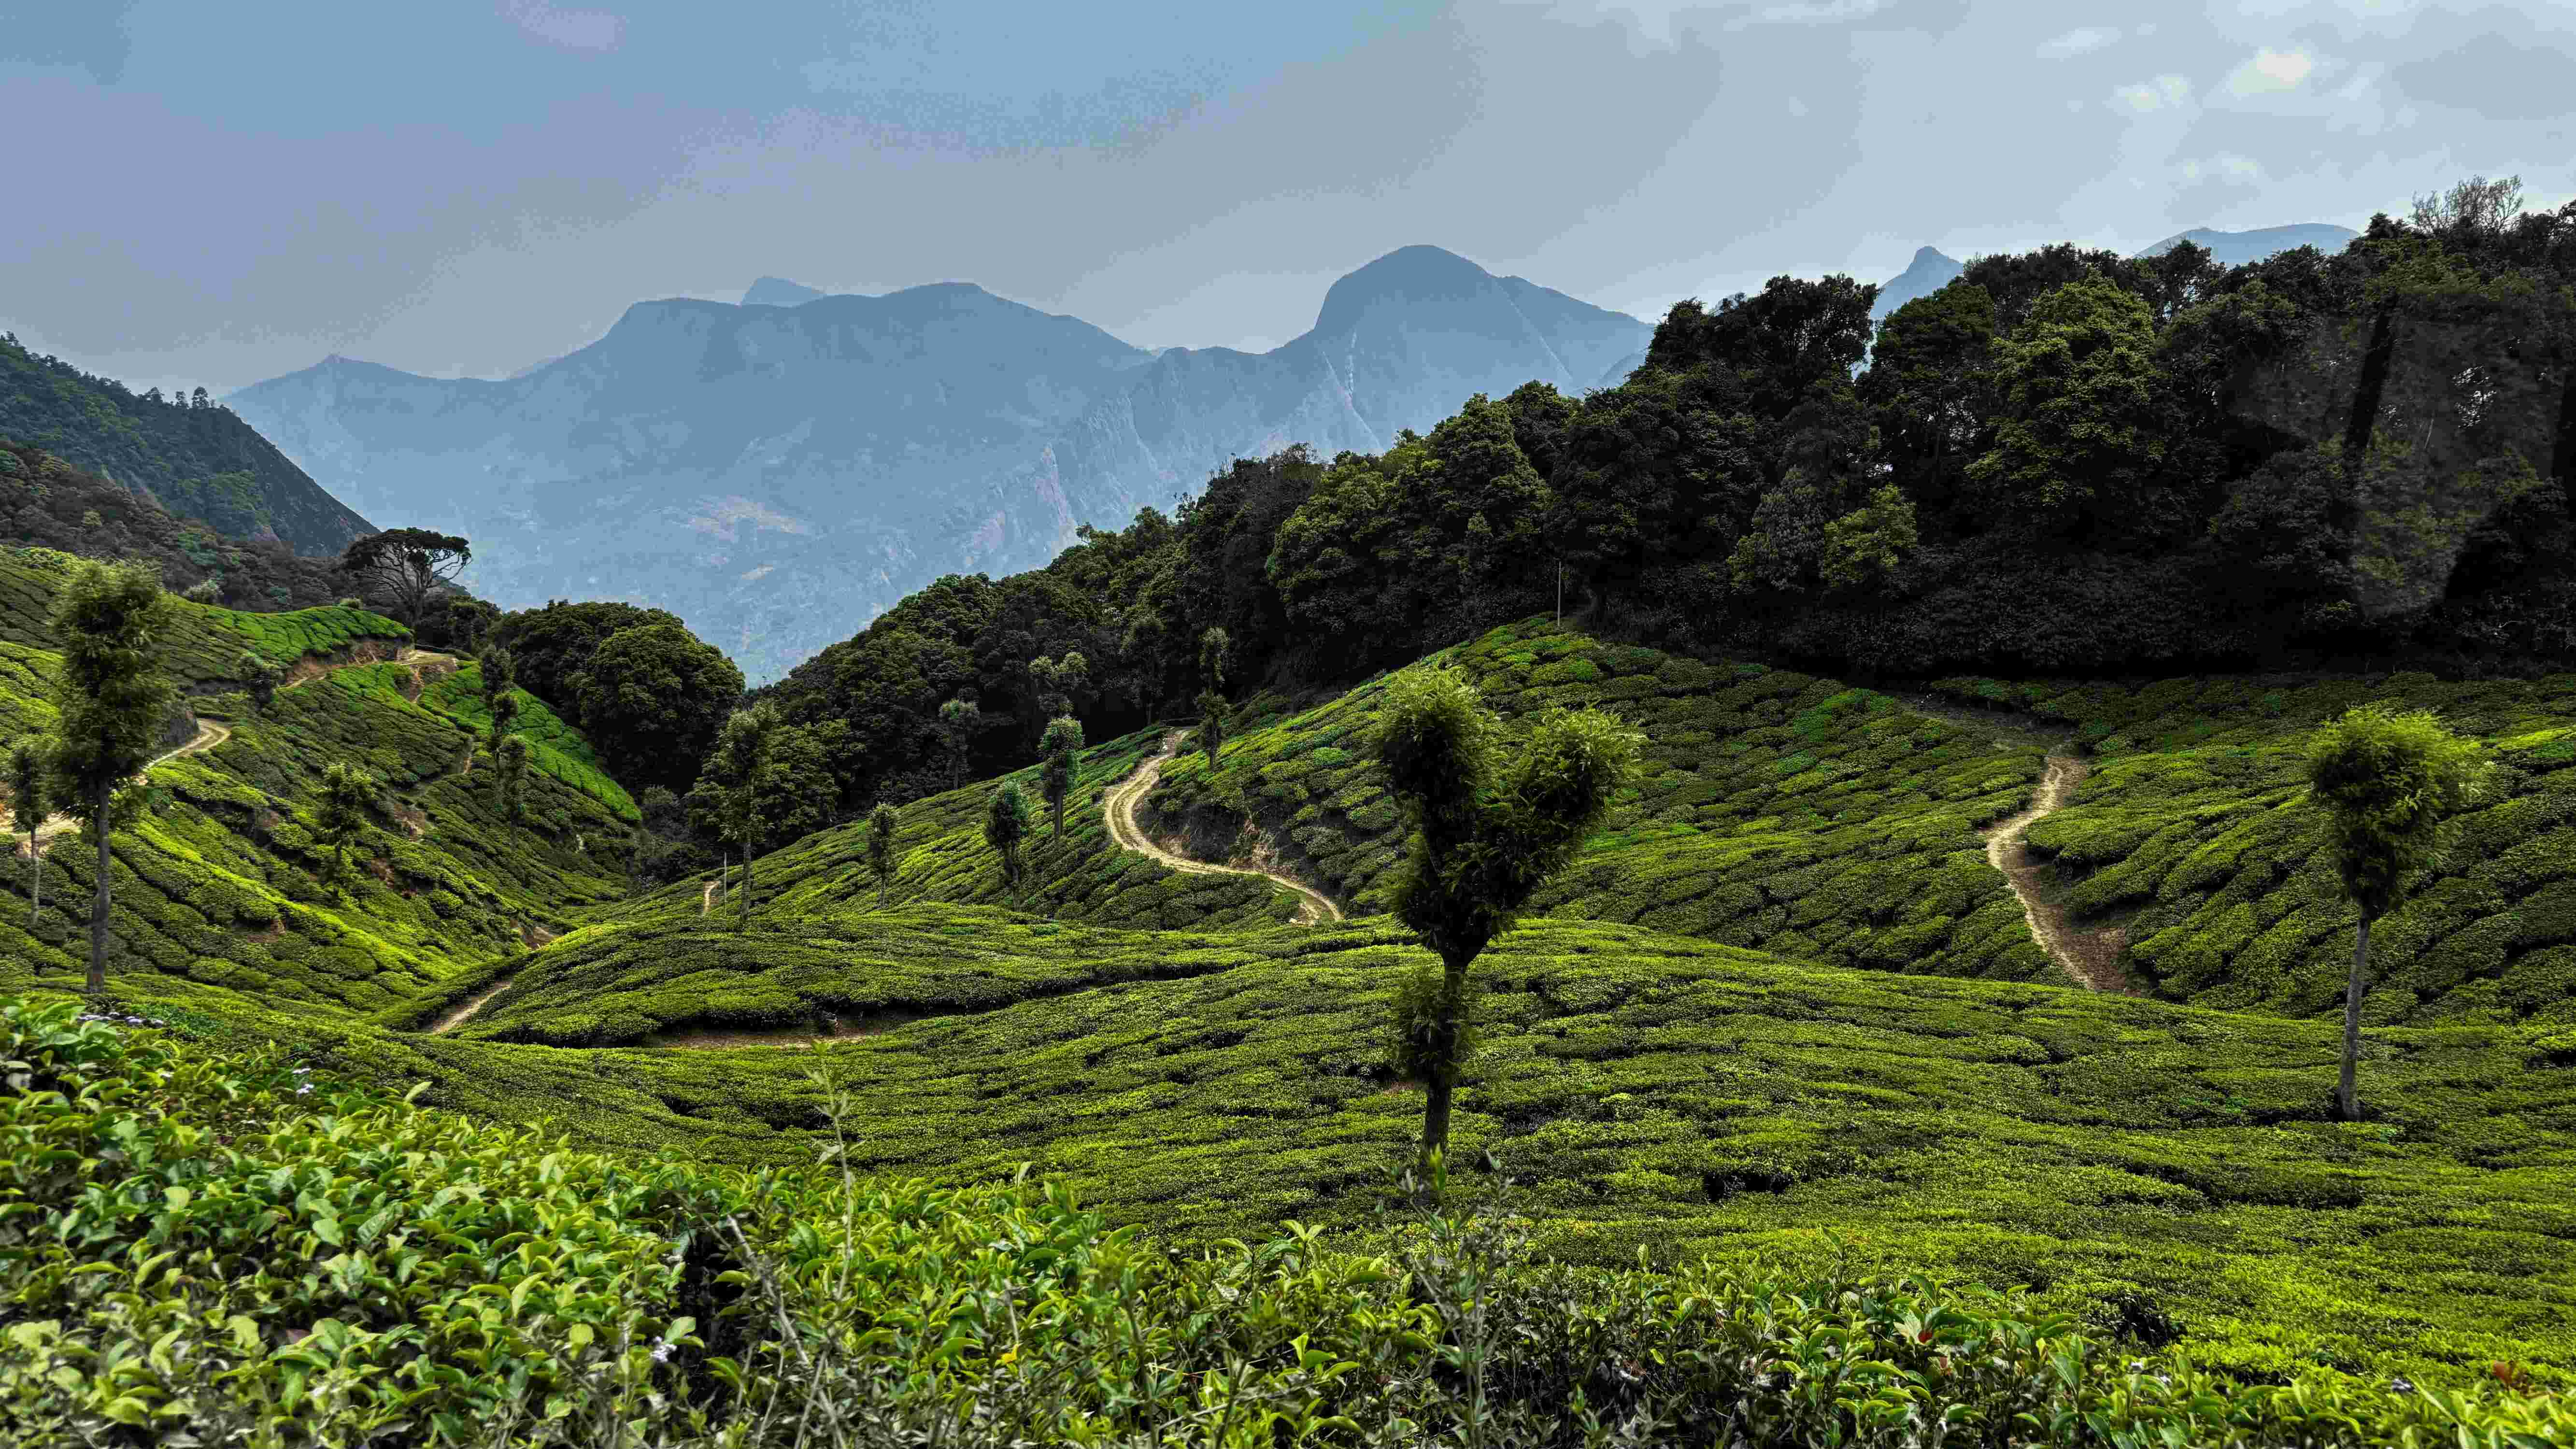
\includegraphics[width=.9\textwidth]{figs/cas-munnar-2024.jpg}
%	\caption{The beauty of Munnar, Kerala. (See also Table \protect\ref{tbl1}).}
%	\label{FIG:2}
%\end{figure*}
%
%
%\subsection[Enumerated ...]{Enumerated and Itemized Lists}
%{cas-dc.cls} provides an extended list processing macros
%which makes the usage a bit more user friendly than the default
%\LaTeX{} list macros.   With an optional argument to the
%\verb+\begin{enumerate}+ command, you can change the list counter
%type and its attributes.
%
%\begin{verbatim}
% \begin{enumerate}[1.]
% \item The enumerate environment starts with an optional
%   argument `1.', so that the item counter will be suffixed
%   by a period.
% \item You can use `a)' for alphabetical counter and '(i)' 
%  for roman counter.
%  \begin{enumerate}[a)]
%    \item Another level of list with alphabetical counter.
%    \item One more item before we start another.
%    \item One more item before we start another.
%    \item One more item before we start another.
%    \item One more item before we start another.
%\end{verbatim}
%
%Further, the enhanced list environment allows one to prefix a
%string like `step' to all the item numbers.  
%
%\begin{verbatim}
% \begin{enumerate}[Step 1.]
%  \item This is the first step of the example list.
%  \item Obviously this is the second step.
%  \item The final step to wind up this example.
% \end{enumerate}
%\end{verbatim}
%
%\subsection{Cross-references}
%In electronic publications, articles may be internally
%hyperlinked. Hyperlinks are generated from proper
%cross-references in the article.  For example, the words
%\textcolor{black!80}{Fig.~1} will never be more than simple text,
%whereas the proper cross-reference \verb+\ref{tiger}+ may be
%turned into a hyperlink to the figure itself:
%\textcolor{blue}{Fig.~1}.  In the same way,
%the words \textcolor{blue}{Ref.~[1]} will fail to turn into a
%hyperlink; the proper cross-reference is \verb+\cite{Knuth96}+.
%Cross-referencing is possible in \LaTeX{} for sections,
%subsections, formulae, figures, tables, and literature
%references.
%
%\subsection{Bibliography}
%
%Two bibliographic style files (\verb+*.bst+) are provided ---
%{model1-num-names.bst} and {model2-names.bst} --- the first one can be
%used for the numbered scheme. This can also be used for the numbered
%with new options of {natbib.sty}. The second one is for the author year
%scheme. When  you use model2-names.bst, the citation commands will be
%like \verb+\citep+,  \verb+\citet+, \verb+\citealt+ etc. However when
%you use model1-num-names.bst, you may use only \verb+\cite+ command.
%
%\verb+thebibliography+ environment.  Each reference is a\linebreak
%\verb+\bibitem+ and each \verb+\bibitem+ is identified by a label,
%by which it can be cited in the text:
%
%\noindent In connection with cross-referencing and
%possible future hyperlinking it is not a good idea to collect
%more that one literature item in one \verb+\bibitem+.  The
%so-called Harvard or author-year style of referencing is enabled
%by the \LaTeX{} package {natbib}. With this package the
%literature can be cited as follows:
%
%\begin{enumerate}[\textbullet]
%\item Parenthetical: \verb+\citep{WB96}+ produces (Wettig \& Brown, 1996).
%\item Textual: \verb+\citet{ESG96}+ produces Elson et al. (1996).
%\item An affix and part of a reference:\break
%\verb+\citep[e.g.][Ch. 2]{Gea97}+ produces (e.g. Governato et
%al., 1997, Ch. 2).
%\end{enumerate}
%
%In the numbered scheme of citation, \verb+\cite{<label>}+ is used,
%since \verb+\citep+ or \verb+\citet+ has no relevance in the numbered
%scheme.  {natbib} package is loaded by {cas-dc} with
%\verb+numbers+ as default option.  You can change this to author-year
%or harvard scheme by adding option \verb+authoryear+ in the class
%loading command.  If you want to use more options of the {natbib}
%package, you can do so with the \verb+\biboptions+ command.  For
%details of various options of the {natbib} package, please take a
%look at the {natbib} documentation, which is part of any standard
%\LaTeX{} installation.
%
%\appendix
%\subsection{My Appendix}
%Appendix sections are coded under \verb+\appendix+.
%
%\verb+\printcredits+ command is used after appendix sections to list 
%author credit taxonomy contribution roles tagged using \verb+\credit+ 
%in frontmatter.

\printcredits

%% Loading bibliography style file
%\bibliographystyle{model1-num-names}
\bibliographystyle{cas-model2-names}

% Loading bibliography database
%\bibliography{cas-refs}
\bibliography{biblio}


%\vskip3pt

\bio{}
Author biography without author photo.
\endbio

\bio{figs/cas-pic1}
Author biography with author photo.
\endbio

\bio{figs/cas-pic1}
Author biography with author photo.
\endbio

\end{document}

